% Options for packages loaded elsewhere
% Options for packages loaded elsewhere
\PassOptionsToPackage{unicode}{hyperref}
\PassOptionsToPackage{hyphens}{url}
\PassOptionsToPackage{dvipsnames,svgnames,x11names}{xcolor}
%
\documentclass[
  letterpaper,
  DIV=11,
  numbers=noendperiod]{scrartcl}
\usepackage{xcolor}
\usepackage{amsmath,amssymb}
\setcounter{secnumdepth}{-\maxdimen} % remove section numbering
\usepackage{iftex}
\ifPDFTeX
  \usepackage[T1]{fontenc}
  \usepackage[utf8]{inputenc}
  \usepackage{textcomp} % provide euro and other symbols
\else % if luatex or xetex
  \usepackage{unicode-math} % this also loads fontspec
  \defaultfontfeatures{Scale=MatchLowercase}
  \defaultfontfeatures[\rmfamily]{Ligatures=TeX,Scale=1}
\fi
\usepackage{lmodern}
\ifPDFTeX\else
  % xetex/luatex font selection
\fi
% Use upquote if available, for straight quotes in verbatim environments
\IfFileExists{upquote.sty}{\usepackage{upquote}}{}
\IfFileExists{microtype.sty}{% use microtype if available
  \usepackage[]{microtype}
  \UseMicrotypeSet[protrusion]{basicmath} % disable protrusion for tt fonts
}{}
\makeatletter
\@ifundefined{KOMAClassName}{% if non-KOMA class
  \IfFileExists{parskip.sty}{%
    \usepackage{parskip}
  }{% else
    \setlength{\parindent}{0pt}
    \setlength{\parskip}{6pt plus 2pt minus 1pt}}
}{% if KOMA class
  \KOMAoptions{parskip=half}}
\makeatother
% Make \paragraph and \subparagraph free-standing
\makeatletter
\ifx\paragraph\undefined\else
  \let\oldparagraph\paragraph
  \renewcommand{\paragraph}{
    \@ifstar
      \xxxParagraphStar
      \xxxParagraphNoStar
  }
  \newcommand{\xxxParagraphStar}[1]{\oldparagraph*{#1}\mbox{}}
  \newcommand{\xxxParagraphNoStar}[1]{\oldparagraph{#1}\mbox{}}
\fi
\ifx\subparagraph\undefined\else
  \let\oldsubparagraph\subparagraph
  \renewcommand{\subparagraph}{
    \@ifstar
      \xxxSubParagraphStar
      \xxxSubParagraphNoStar
  }
  \newcommand{\xxxSubParagraphStar}[1]{\oldsubparagraph*{#1}\mbox{}}
  \newcommand{\xxxSubParagraphNoStar}[1]{\oldsubparagraph{#1}\mbox{}}
\fi
\makeatother

\usepackage{color}
\usepackage{fancyvrb}
\newcommand{\VerbBar}{|}
\newcommand{\VERB}{\Verb[commandchars=\\\{\}]}
\DefineVerbatimEnvironment{Highlighting}{Verbatim}{commandchars=\\\{\}}
% Add ',fontsize=\small' for more characters per line
\usepackage{framed}
\definecolor{shadecolor}{RGB}{241,243,245}
\newenvironment{Shaded}{\begin{snugshade}}{\end{snugshade}}
\newcommand{\AlertTok}[1]{\textcolor[rgb]{0.68,0.00,0.00}{#1}}
\newcommand{\AnnotationTok}[1]{\textcolor[rgb]{0.37,0.37,0.37}{#1}}
\newcommand{\AttributeTok}[1]{\textcolor[rgb]{0.40,0.45,0.13}{#1}}
\newcommand{\BaseNTok}[1]{\textcolor[rgb]{0.68,0.00,0.00}{#1}}
\newcommand{\BuiltInTok}[1]{\textcolor[rgb]{0.00,0.23,0.31}{#1}}
\newcommand{\CharTok}[1]{\textcolor[rgb]{0.13,0.47,0.30}{#1}}
\newcommand{\CommentTok}[1]{\textcolor[rgb]{0.37,0.37,0.37}{#1}}
\newcommand{\CommentVarTok}[1]{\textcolor[rgb]{0.37,0.37,0.37}{\textit{#1}}}
\newcommand{\ConstantTok}[1]{\textcolor[rgb]{0.56,0.35,0.01}{#1}}
\newcommand{\ControlFlowTok}[1]{\textcolor[rgb]{0.00,0.23,0.31}{\textbf{#1}}}
\newcommand{\DataTypeTok}[1]{\textcolor[rgb]{0.68,0.00,0.00}{#1}}
\newcommand{\DecValTok}[1]{\textcolor[rgb]{0.68,0.00,0.00}{#1}}
\newcommand{\DocumentationTok}[1]{\textcolor[rgb]{0.37,0.37,0.37}{\textit{#1}}}
\newcommand{\ErrorTok}[1]{\textcolor[rgb]{0.68,0.00,0.00}{#1}}
\newcommand{\ExtensionTok}[1]{\textcolor[rgb]{0.00,0.23,0.31}{#1}}
\newcommand{\FloatTok}[1]{\textcolor[rgb]{0.68,0.00,0.00}{#1}}
\newcommand{\FunctionTok}[1]{\textcolor[rgb]{0.28,0.35,0.67}{#1}}
\newcommand{\ImportTok}[1]{\textcolor[rgb]{0.00,0.46,0.62}{#1}}
\newcommand{\InformationTok}[1]{\textcolor[rgb]{0.37,0.37,0.37}{#1}}
\newcommand{\KeywordTok}[1]{\textcolor[rgb]{0.00,0.23,0.31}{\textbf{#1}}}
\newcommand{\NormalTok}[1]{\textcolor[rgb]{0.00,0.23,0.31}{#1}}
\newcommand{\OperatorTok}[1]{\textcolor[rgb]{0.37,0.37,0.37}{#1}}
\newcommand{\OtherTok}[1]{\textcolor[rgb]{0.00,0.23,0.31}{#1}}
\newcommand{\PreprocessorTok}[1]{\textcolor[rgb]{0.68,0.00,0.00}{#1}}
\newcommand{\RegionMarkerTok}[1]{\textcolor[rgb]{0.00,0.23,0.31}{#1}}
\newcommand{\SpecialCharTok}[1]{\textcolor[rgb]{0.37,0.37,0.37}{#1}}
\newcommand{\SpecialStringTok}[1]{\textcolor[rgb]{0.13,0.47,0.30}{#1}}
\newcommand{\StringTok}[1]{\textcolor[rgb]{0.13,0.47,0.30}{#1}}
\newcommand{\VariableTok}[1]{\textcolor[rgb]{0.07,0.07,0.07}{#1}}
\newcommand{\VerbatimStringTok}[1]{\textcolor[rgb]{0.13,0.47,0.30}{#1}}
\newcommand{\WarningTok}[1]{\textcolor[rgb]{0.37,0.37,0.37}{\textit{#1}}}

\usepackage{longtable,booktabs,array}
\usepackage{calc} % for calculating minipage widths
% Correct order of tables after \paragraph or \subparagraph
\usepackage{etoolbox}
\makeatletter
\patchcmd\longtable{\par}{\if@noskipsec\mbox{}\fi\par}{}{}
\makeatother
% Allow footnotes in longtable head/foot
\IfFileExists{footnotehyper.sty}{\usepackage{footnotehyper}}{\usepackage{footnote}}
\makesavenoteenv{longtable}
\usepackage{graphicx}
\makeatletter
\newsavebox\pandoc@box
\newcommand*\pandocbounded[1]{% scales image to fit in text height/width
  \sbox\pandoc@box{#1}%
  \Gscale@div\@tempa{\textheight}{\dimexpr\ht\pandoc@box+\dp\pandoc@box\relax}%
  \Gscale@div\@tempb{\linewidth}{\wd\pandoc@box}%
  \ifdim\@tempb\p@<\@tempa\p@\let\@tempa\@tempb\fi% select the smaller of both
  \ifdim\@tempa\p@<\p@\scalebox{\@tempa}{\usebox\pandoc@box}%
  \else\usebox{\pandoc@box}%
  \fi%
}
% Set default figure placement to htbp
\def\fps@figure{htbp}
\makeatother





\setlength{\emergencystretch}{3em} % prevent overfull lines

\providecommand{\tightlist}{%
  \setlength{\itemsep}{0pt}\setlength{\parskip}{0pt}}



 



\usepackage{fancyvrb}
\usepackage{tcolorbox}
\usepackage{fontspec}
\usepackage{enumitem}
\usepackage{amsmath}
\usepackage{amssymb}
\usepackage{amsthm}
\usepackage{graphicx}
\usepackage{hyperref}
\usepackage{pdflscape}

% Set main font to Palatino Linotype
\setmainfont{Palatino Linotype}

% Define code output environment with smaller font size
\newenvironment{codeoutput}{\begin{tcolorbox}[colback=white!95!blue!5, colframe=blue!20!black, boxrule=0.5pt, arc=4pt, fontupper=\footnotesize]}{\end{tcolorbox}}

% Define callout boxes
\newenvironment{calloutorange}{\begin{tcolorbox}[colback=yellow!10, colframe=orange, arc=4pt]}{\end{tcolorbox}}
\newenvironment{calloutgrey}{\begin{tcolorbox}[colback=gray!10, colframe=black!50, arc=4pt]}{\end{tcolorbox}}

% Define important formula environment
\newenvironment{importantformula}{\begin{tcolorbox}[colback=white, colframe=black!50, arc=4pt]}{\end{tcolorbox}}

% Define exercise box environment
\newenvironment{exercisebox}{\begin{tcolorbox}[colback=gray!10, colframe=black!50, boxrule=0.5pt, arc=4pt, left=5pt, right=5pt, top=5pt, bottom=5pt]}{\end{tcolorbox}}

% Define blockquote environment
\newenvironment{blockquote}{\begin{tcolorbox}[colback=gray!10, colframe=black!50, boxrule=0.5pt, arc=4pt]}{\end{tcolorbox}}

% Define centered text environment
\newenvironment{centeredtext}{\begin{center}}{\end{center}}

% Define custom list environment without lineheight option
\newlist{customitemize}{itemize}{1}
\setlist[customitemize,1]{label=\textbullet, left=0pt, itemsep=0.2em, parsep=0pt, topsep=0pt}

\newlist{customenumerate}{enumerate}{1}
\setlist[customenumerate,1]{label=\arabic*., left=0pt, itemsep=0.2em, parsep=0pt, topsep=0pt}
\usepackage{booktabs}
\usepackage{longtable}
\usepackage{array}
\usepackage{multirow}
\usepackage{wrapfig}
\usepackage{float}
\usepackage{colortbl}
\usepackage{pdflscape}
\usepackage{tabu}
\usepackage{threeparttable}
\usepackage{threeparttablex}
\usepackage[normalem]{ulem}
\usepackage{makecell}
\usepackage{xcolor}
\KOMAoption{captions}{tableheading}
\makeatletter
\@ifpackageloaded{caption}{}{\usepackage{caption}}
\AtBeginDocument{%
\ifdefined\contentsname
  \renewcommand*\contentsname{Table of contents}
\else
  \newcommand\contentsname{Table of contents}
\fi
\ifdefined\listfigurename
  \renewcommand*\listfigurename{List of Figures}
\else
  \newcommand\listfigurename{List of Figures}
\fi
\ifdefined\listtablename
  \renewcommand*\listtablename{List of Tables}
\else
  \newcommand\listtablename{List of Tables}
\fi
\ifdefined\figurename
  \renewcommand*\figurename{Figure}
\else
  \newcommand\figurename{Figure}
\fi
\ifdefined\tablename
  \renewcommand*\tablename{Table}
\else
  \newcommand\tablename{Table}
\fi
}
\@ifpackageloaded{float}{}{\usepackage{float}}
\floatstyle{ruled}
\@ifundefined{c@chapter}{\newfloat{codelisting}{h}{lop}}{\newfloat{codelisting}{h}{lop}[chapter]}
\floatname{codelisting}{Listing}
\newcommand*\listoflistings{\listof{codelisting}{List of Listings}}
\makeatother
\makeatletter
\makeatother
\makeatletter
\@ifpackageloaded{caption}{}{\usepackage{caption}}
\@ifpackageloaded{subcaption}{}{\usepackage{subcaption}}
\makeatother
\usepackage{bookmark}
\IfFileExists{xurl.sty}{\usepackage{xurl}}{} % add URL line breaks if available
\urlstyle{same}
\hypersetup{
  pdftitle={Matrix Algebra},
  colorlinks=true,
  linkcolor={blue},
  filecolor={Maroon},
  citecolor={Blue},
  urlcolor={Blue},
  pdfcreator={LaTeX via pandoc}}


\title{Matrix Algebra}
\author{}
\date{}
\begin{document}
\maketitle


This document is a summary of different stats courses:

\begin{itemize}
\tightlist
\item
  Introduction to Linear Models and Matrix Algebra (HarvardX PH525.2x
  via Edx) There is a free e-book which contains the full course:
  dataanalysisforthelifesciences.pdf and all the code can be found in
  the git of the author.
\end{itemize}

\section{Introduction}\label{introduction}

\emph{Scalars}: are numbers, for example 3, or -9.898

\emph{Vectors}: are series of numbers. For example (3,5,6.7,-1)

\emph{Matrices}: are a series of vectors. We generally use \texttt{X} to
represent a matrix, and a matrix will have \texttt{N} rows and
\texttt{p} columns A square matrix has the same number of rows as
columns. For example a matrix of 3 rows and 3 columns (3x3):

\[
\begin{pmatrix}
1 & 1 & 1.6 \\
3 & -2 & 0 \\
2 & 1 & -1
\end{pmatrix}
\]

\section{Magnitude of a vector}\label{magnitude-of-a-vector}

The magnitude of a vector represents its length in space. The magnitude
(also called the Euclidean norm) is calculated using the square root of
the sum of the squares of its components.

For a vector: \(\vec{v} = [v_1,v_2,\cdots,v_n]\) \[
\|\vec{v}\| = \sqrt{v_1^2 + v_2^2 + \dots + v_n^2} = \sqrt{\sum_{i=1}^{n} v_i^2}
\] Example: \[
\vec{v} = [3, 4]
\]

Then:

\[
\|\vec{v}\| = \sqrt{3^2 + 4^2} = \sqrt{9 + 16} = \sqrt{25} = 5
\]

\begin{center}
\pandocbounded{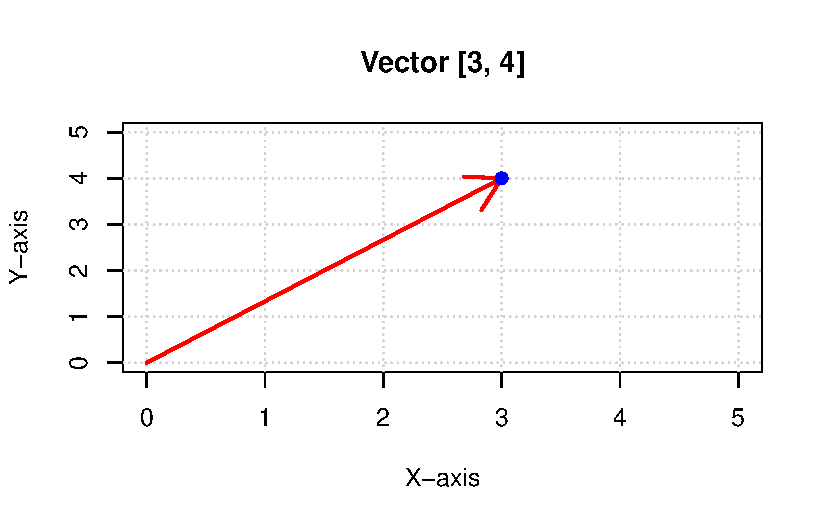
\includegraphics[keepaspectratio]{matrix_files/figure-pdf/unnamed-chunk-2-1.pdf}}
\end{center}

\begin{Shaded}
\begin{Highlighting}[]
\CommentTok{\# Define the vector}
\NormalTok{v }\OtherTok{\textless{}{-}} \FunctionTok{c}\NormalTok{(}\DecValTok{3}\NormalTok{, }\DecValTok{4}\NormalTok{)}

\CommentTok{\# Calculate the magnitude (Euclidean norm)}
\NormalTok{(magnitude }\OtherTok{\textless{}{-}} \FunctionTok{sqrt}\NormalTok{(}\FunctionTok{sum}\NormalTok{(v}\SpecialCharTok{\^{}}\DecValTok{2}\NormalTok{)))}
\end{Highlighting}
\end{Shaded}

\begin{verbatim}
[1] 5
\end{verbatim}

\section{Dot product of vectors}\label{dot-product-of-vectors}

The dot product is one way of multiplying two or more vectors. The
resultant of the dot product of vectors is a scalar quantity. Thus, the
dot product is also known as a scalar product.

Geometrically, the dot product of two vectors is the product of their
Euclidean magnitudes and the cosine of the angle between them.

\[
\vec{a} \cdot \vec{b} = \|\vec{a}\| \|\vec{b}\| \cos(\theta)
\]

\begin{center}
\pandocbounded{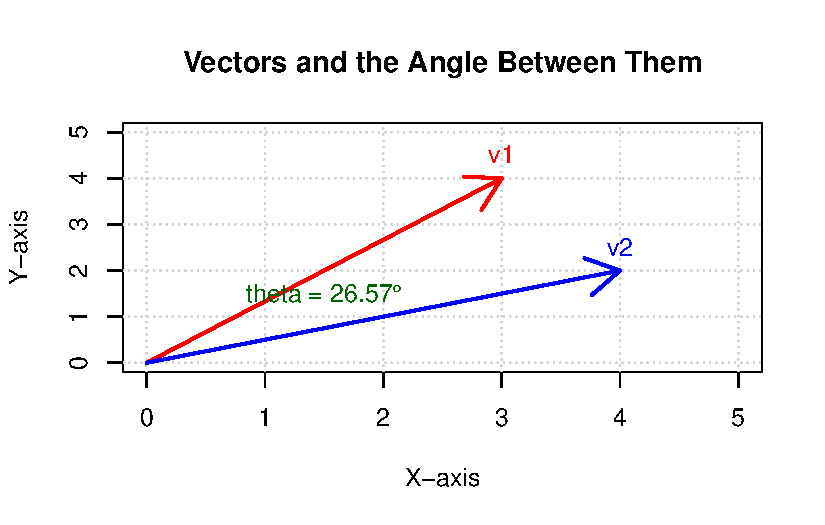
\includegraphics[keepaspectratio]{matrix_files/figure-pdf/unnamed-chunk-4-1.pdf}}
\end{center}

Algebraically, it is the sum of the products of the corresponding
entries of two sequences of numbers.

\[
\vec{a} \cdot \vec{b} = \sum_{i=1}^{n} a_i b_i = a_1b_1 + a_2b_2 + \dots + a_n b_n
\]

Example:

Let:

\[
\vec{a} = [1, 2, 3], \quad \vec{b} = [4, 5, 6]
\]

Then:

\[
\vec{a} \cdot \vec{b} = 1 \cdot 4 + 2 \cdot 5 + 3 \cdot 6 = 4 + 10 + 18 = 32
\] in \texttt{r}

\begin{Shaded}
\begin{Highlighting}[]
\CommentTok{\# Define the vectors}
\NormalTok{a }\OtherTok{\textless{}{-}} \FunctionTok{c}\NormalTok{(}\DecValTok{1}\NormalTok{, }\DecValTok{2}\NormalTok{, }\DecValTok{3}\NormalTok{)}
\NormalTok{b }\OtherTok{\textless{}{-}} \FunctionTok{c}\NormalTok{(}\DecValTok{4}\NormalTok{, }\DecValTok{5}\NormalTok{, }\DecValTok{6}\NormalTok{)}

\CommentTok{\# Compute the dot product}
\NormalTok{dot\_product }\OtherTok{\textless{}{-}} \FunctionTok{sum}\NormalTok{(a }\SpecialCharTok{*}\NormalTok{ b)}
\NormalTok{dot\_product}
\end{Highlighting}
\end{Shaded}

\begin{verbatim}
[1] 32
\end{verbatim}

\section{Cosine Similarity}\label{cosine-similarity}

Cosine similarity is a measure of similarity between two non-zero
vectors of an inner product space. It is defined as the cosine of the
angle between the two vectors. This measure is particularly used in text
analysis to measure the similarity between documents.

\begin{Shaded}
\begin{Highlighting}[]
\CommentTok{\# Define vectors}
\NormalTok{v1 }\OtherTok{\textless{}{-}} \FunctionTok{c}\NormalTok{(}\DecValTok{3}\NormalTok{, }\DecValTok{4}\NormalTok{)}
\NormalTok{v2 }\OtherTok{\textless{}{-}} \FunctionTok{c}\NormalTok{(}\DecValTok{4}\NormalTok{, }\DecValTok{2}\NormalTok{)}

\CommentTok{\# Calculate angle}
\NormalTok{dot }\OtherTok{\textless{}{-}} \FunctionTok{sum}\NormalTok{(v1 }\SpecialCharTok{*}\NormalTok{ v2)}
\NormalTok{mag1 }\OtherTok{\textless{}{-}} \FunctionTok{sqrt}\NormalTok{(}\FunctionTok{sum}\NormalTok{(v1}\SpecialCharTok{\^{}}\DecValTok{2}\NormalTok{))}
\NormalTok{mag2 }\OtherTok{\textless{}{-}} \FunctionTok{sqrt}\NormalTok{(}\FunctionTok{sum}\NormalTok{(v2}\SpecialCharTok{\^{}}\DecValTok{2}\NormalTok{))}
\NormalTok{angle }\OtherTok{\textless{}{-}} \FunctionTok{acos}\NormalTok{(dot }\SpecialCharTok{/}\NormalTok{ (mag1 }\SpecialCharTok{*}\NormalTok{ mag2)) }\SpecialCharTok{*} \DecValTok{180} \SpecialCharTok{/}\NormalTok{ pi}

\CommentTok{\# Plot}
\FunctionTok{plot}\NormalTok{(}\DecValTok{0}\NormalTok{, }\DecValTok{0}\NormalTok{, }\AttributeTok{xlim =} \FunctionTok{c}\NormalTok{(}\DecValTok{0}\NormalTok{, }\DecValTok{5}\NormalTok{), }\AttributeTok{ylim =} \FunctionTok{c}\NormalTok{(}\DecValTok{0}\NormalTok{, }\DecValTok{5}\NormalTok{), }\AttributeTok{type =} \StringTok{"n"}\NormalTok{,}
     \AttributeTok{xlab =} \StringTok{"X{-}axis"}\NormalTok{, }\AttributeTok{ylab =} \StringTok{"Y{-}axis"}\NormalTok{, }\AttributeTok{main =} \StringTok{"Vectors and Angle"}\NormalTok{)}
\FunctionTok{grid}\NormalTok{()}
\FunctionTok{arrows}\NormalTok{(}\DecValTok{0}\NormalTok{, }\DecValTok{0}\NormalTok{, v1[}\DecValTok{1}\NormalTok{], v1[}\DecValTok{2}\NormalTok{], }\AttributeTok{col =} \StringTok{"red"}\NormalTok{, }\AttributeTok{lwd =} \DecValTok{2}\NormalTok{)}
\FunctionTok{arrows}\NormalTok{(}\DecValTok{0}\NormalTok{, }\DecValTok{0}\NormalTok{, v2[}\DecValTok{1}\NormalTok{], v2[}\DecValTok{2}\NormalTok{], }\AttributeTok{col =} \StringTok{"blue"}\NormalTok{, }\AttributeTok{lwd =} \DecValTok{2}\NormalTok{)}
\FunctionTok{text}\NormalTok{(v1[}\DecValTok{1}\NormalTok{], v1[}\DecValTok{2}\NormalTok{], }\StringTok{"v1"}\NormalTok{, }\AttributeTok{pos =} \DecValTok{3}\NormalTok{, }\AttributeTok{col =} \StringTok{"red"}\NormalTok{)}
\FunctionTok{text}\NormalTok{(v2[}\DecValTok{1}\NormalTok{], v2[}\DecValTok{2}\NormalTok{], }\StringTok{"v2"}\NormalTok{, }\AttributeTok{pos =} \DecValTok{3}\NormalTok{, }\AttributeTok{col =} \StringTok{"blue"}\NormalTok{)}
\FunctionTok{text}\NormalTok{(}\FloatTok{1.5}\NormalTok{, }\FloatTok{1.5}\NormalTok{, }\FunctionTok{paste0}\NormalTok{(}\StringTok{"θ = "}\NormalTok{, }\FunctionTok{round}\NormalTok{(angle, }\DecValTok{2}\NormalTok{), }\StringTok{"°"}\NormalTok{), }\AttributeTok{col =} \StringTok{"darkgreen"}\NormalTok{)}
\end{Highlighting}
\end{Shaded}

\pandocbounded{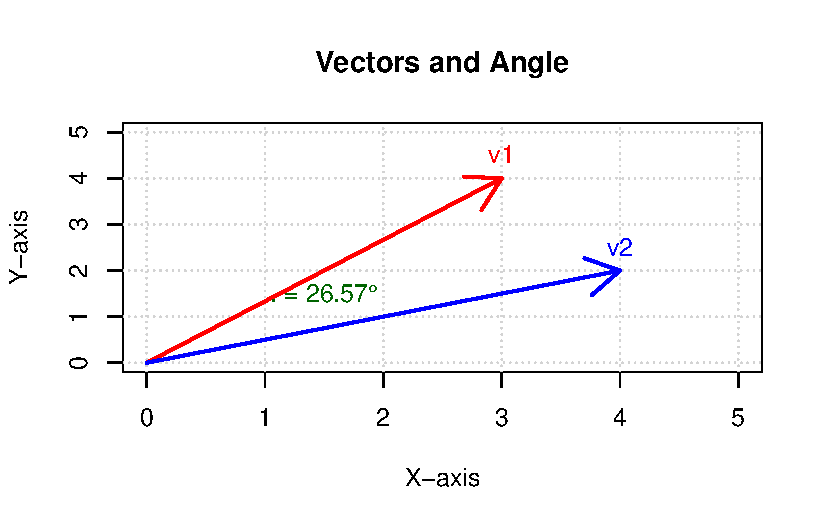
\includegraphics[keepaspectratio]{matrix_files/figure-pdf/unnamed-chunk-6-1.pdf}}

The cosine similarity between two vectors \textbf{a} and \textbf{b} is
calculated as:

\[
\text{cosine similarity} = \cos(\theta) = \frac{\vec{a} \cdot \vec{b}}{\|\vec{a}\| \|\vec{b}\|}
\] Where: - \(\vec{a} \cdot \vec{b}\) is the dot product of vectors
\textbf{a} and \textbf{b} - \(\|\vec{a}\|\) and \(\|\vec{b}\|\) are the
magnitudes (Euclidean norms) of vectors \textbf{a} and \textbf{b} -
\(\theta\) is the angle between the vectors

\[
\vec{a} \cdot \vec{b} = \sum_{i=1}^{n} a_i b_i = a_1b_1 + a_2b_2 + \dots + a_nb_n
\] \[
\|\vec{v}\| = \sqrt{v_1^2 + v_2^2 + \dots + v_n^2} = \sqrt{\sum_{i=1}^{n} v_i^2}
\]

\begin{center}
\pandocbounded{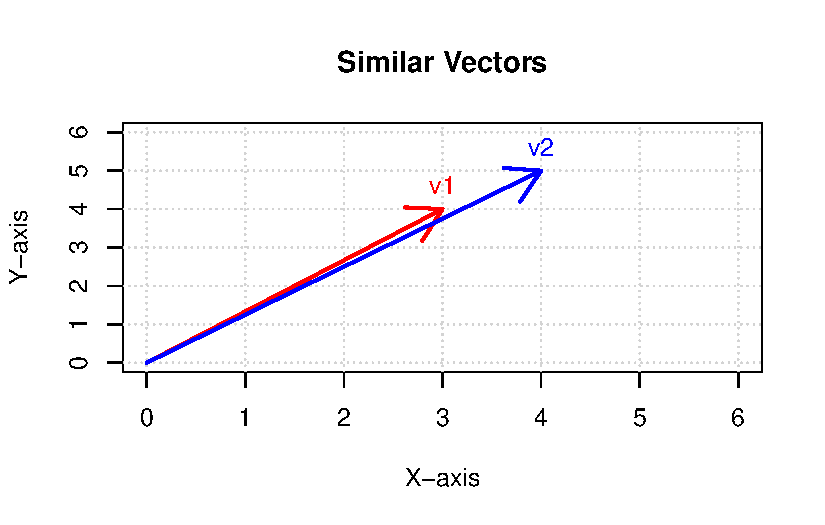
\includegraphics[keepaspectratio]{matrix_files/figure-pdf/unnamed-chunk-7-1.pdf}}
\end{center}

These vectors point in nearly the same direction, forming a small angle
between them. This results in a cosine similarity close to 1, indicating
high similarity.

\begin{center}
\pandocbounded{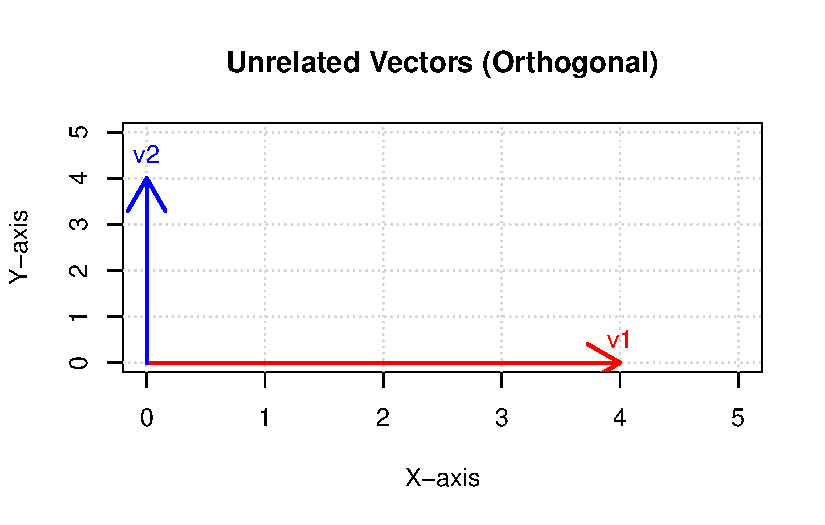
\includegraphics[keepaspectratio]{matrix_files/figure-pdf/unnamed-chunk-8-1.pdf}}
\end{center}

These vectors are perpendicular to each other, forming a 90° angle.
Their cosine similarity is 0, meaning they are completely unrelated in
direction.

\begin{center}
\pandocbounded{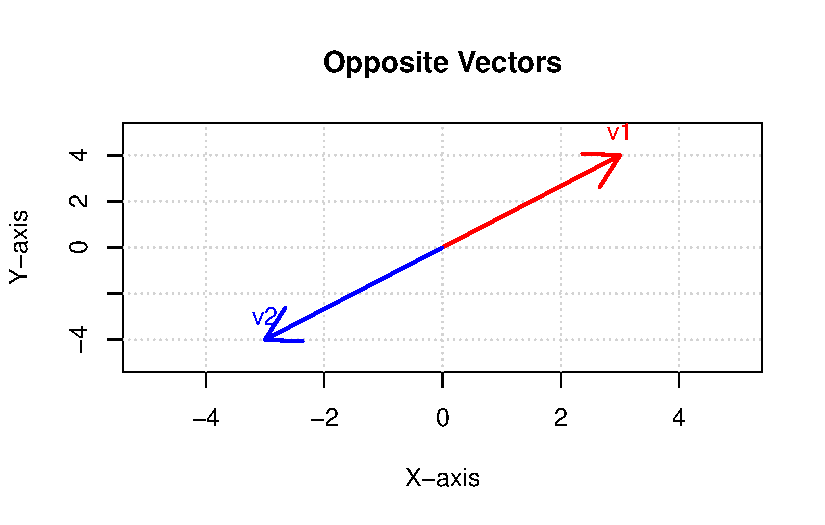
\includegraphics[keepaspectratio]{matrix_files/figure-pdf/unnamed-chunk-9-1.pdf}}
\end{center}

These vectors point in exactly opposite directions, forming a 180°
angle. Their cosine similarity is -1, indicating they are completely
dissimilar in direction.

We can calculate this in \texttt{r} manually:

\begin{Shaded}
\begin{Highlighting}[]
\CommentTok{\# Define vectors}
\NormalTok{a }\OtherTok{\textless{}{-}} \FunctionTok{c}\NormalTok{(}\DecValTok{1}\NormalTok{, }\DecValTok{2}\NormalTok{, }\DecValTok{3}\NormalTok{)}
\NormalTok{b }\OtherTok{\textless{}{-}} \FunctionTok{c}\NormalTok{(}\DecValTok{4}\NormalTok{, }\DecValTok{5}\NormalTok{, }\DecValTok{6}\NormalTok{)}

\CommentTok{\# Dot product}
\NormalTok{dot\_product }\OtherTok{\textless{}{-}} \FunctionTok{sum}\NormalTok{(a }\SpecialCharTok{*}\NormalTok{ b)}

\CommentTok{\# Magnitudes}
\NormalTok{mag\_a }\OtherTok{\textless{}{-}} \FunctionTok{sqrt}\NormalTok{(}\FunctionTok{sum}\NormalTok{(a}\SpecialCharTok{\^{}}\DecValTok{2}\NormalTok{))}
\NormalTok{mag\_b }\OtherTok{\textless{}{-}} \FunctionTok{sqrt}\NormalTok{(}\FunctionTok{sum}\NormalTok{(b}\SpecialCharTok{\^{}}\DecValTok{2}\NormalTok{))}

\CommentTok{\# Cosine similarity}
\NormalTok{cos\_sim }\OtherTok{\textless{}{-}}\NormalTok{ dot\_product }\SpecialCharTok{/}\NormalTok{ (mag\_a }\SpecialCharTok{*}\NormalTok{ mag\_b)}
\NormalTok{cos\_sim}
\end{Highlighting}
\end{Shaded}

\begin{verbatim}
[1] 0.9746318
\end{verbatim}

or we can use the \texttt{cosine} function from the \texttt{lsa}
package:

\begin{Shaded}
\begin{Highlighting}[]
\NormalTok{x }\OtherTok{\textless{}{-}} \FunctionTok{c}\NormalTok{(}\FloatTok{0.12}\NormalTok{, }\FloatTok{0.44}\NormalTok{, }\FloatTok{0.5}\NormalTok{, }\FloatTok{0.3}\NormalTok{, }\FloatTok{0.7}\NormalTok{, }\FloatTok{0.04}\NormalTok{, }\FloatTok{0.9}\NormalTok{, }\FloatTok{0.8}\NormalTok{)}
\NormalTok{y }\OtherTok{\textless{}{-}} \FunctionTok{c}\NormalTok{(}\FloatTok{0.24}\NormalTok{, }\FloatTok{0.5}\NormalTok{, }\FloatTok{0.7}\NormalTok{, }\FloatTok{0.21}\NormalTok{, }\FloatTok{0.69}\NormalTok{, }\FloatTok{0.2}\NormalTok{, }\FloatTok{0.7}\NormalTok{, }\FloatTok{0.5}\NormalTok{)}

\NormalTok{lsa}\SpecialCharTok{::}\FunctionTok{cosine}\NormalTok{(x, y)}
\end{Highlighting}
\end{Shaded}

\begin{verbatim}
          [,1]
[1,] 0.9551402
\end{verbatim}

Creating a basic search engine

We illustrate a simple example of machine learning by using cosine
similarity to determine which product description is most correlated
with a given search sentence. This basic technique forms the foundation
for many text-based similarity and recommendation systems.

We begin by defining 10 product descriptions:

\begin{Shaded}
\begin{Highlighting}[]
\NormalTok{products }\OtherTok{\textless{}{-}} \FunctionTok{c}\NormalTok{(}
  \StringTok{"Sleek red smartphone with powerful battery and excellent display"}\NormalTok{,}
  \StringTok{"Lightweight laptop with fast performance and long battery life"}\NormalTok{,}
  \StringTok{"Noise{-}cancelling wireless headphones with dynamic sound"}\NormalTok{,}
  \StringTok{"Durable smartwatch with fitness tracking features and water resistance"}\NormalTok{,}
  \StringTok{"Waterproof fitness tracker with heart rate monitoring and step counter"}\NormalTok{,}
  \StringTok{"High resolution tablet with slim design and vibrant colors"}\NormalTok{,}
  \StringTok{"Compact digital camera with optical image stabilization and zoom"}\NormalTok{,}
  \StringTok{"Portable Bluetooth speaker with deep bass and clear audio"}\NormalTok{,}
  \StringTok{"Smart home hub connecting all smart devices seamlessly"}\NormalTok{,}
  \StringTok{"Lightweight e{-}reader with adjustable backlight and user friendly interface"}
\NormalTok{)}
\NormalTok{products}
\end{Highlighting}
\end{Shaded}

\begin{verbatim}
 [1] "Sleek red smartphone with powerful battery and excellent display"          
 [2] "Lightweight laptop with fast performance and long battery life"            
 [3] "Noise-cancelling wireless headphones with dynamic sound"                   
 [4] "Durable smartwatch with fitness tracking features and water resistance"    
 [5] "Waterproof fitness tracker with heart rate monitoring and step counter"    
 [6] "High resolution tablet with slim design and vibrant colors"                
 [7] "Compact digital camera with optical image stabilization and zoom"          
 [8] "Portable Bluetooth speaker with deep bass and clear audio"                 
 [9] "Smart home hub connecting all smart devices seamlessly"                    
[10] "Lightweight e-reader with adjustable backlight and user friendly interface"
\end{verbatim}

\begin{enumerate}
\def\labelenumi{\arabic{enumi}.}
\tightlist
\item
  Tokenization and Vectorization
\end{enumerate}

We define a helper function to tokenize the text (by converting to
lowercase, removing punctuation, and splitting into words). We then
build a vocabulary from both the product descriptions and the search
sentence, and create bag-of-words vectors that count occurrences of each
vocabulary word.

\begin{Shaded}
\begin{Highlighting}[]
\CommentTok{\# Function to tokenize a text string}
\NormalTok{tokenize }\OtherTok{\textless{}{-}} \ControlFlowTok{function}\NormalTok{(text) \{}
  \CommentTok{\# Convert to lower case and remove punctuation (keeping only a{-}z and space)}
\NormalTok{  words }\OtherTok{\textless{}{-}} \FunctionTok{gsub}\NormalTok{(}\StringTok{"[\^{}a{-}z ]"}\NormalTok{, }\StringTok{""}\NormalTok{, }\FunctionTok{tolower}\NormalTok{(text))}
  \FunctionTok{unlist}\NormalTok{(}\FunctionTok{strsplit}\NormalTok{(words, }\StringTok{"}\SpecialCharTok{\textbackslash{}\textbackslash{}}\StringTok{s+"}\NormalTok{))}
\NormalTok{\}}

\CommentTok{\# Tokenize the product descriptions}
\NormalTok{tokenized\_products }\OtherTok{\textless{}{-}} \FunctionTok{lapply}\NormalTok{(products, tokenize)}

\CommentTok{\#print one example:}
\NormalTok{tokenized\_products[}\DecValTok{1}\NormalTok{]}
\end{Highlighting}
\end{Shaded}

\begin{verbatim}
[[1]]
[1] "sleek"      "red"        "smartphone" "with"       "powerful"  
[6] "battery"    "and"        "excellent"  "display"   
\end{verbatim}

\begin{Shaded}
\begin{Highlighting}[]
\CommentTok{\# Define a search sentence}
\NormalTok{search\_sentence }\OtherTok{\textless{}{-}} \StringTok{"Looking for a smartphone with a powerful battery"}
\NormalTok{tokenized\_search }\OtherTok{\textless{}{-}} \FunctionTok{tokenize}\NormalTok{(search\_sentence)}

\CommentTok{\# Create a vocabulary from all tokens in products and search sentence}
\NormalTok{vocab }\OtherTok{\textless{}{-}} \FunctionTok{unique}\NormalTok{(}\FunctionTok{c}\NormalTok{(}\FunctionTok{unlist}\NormalTok{(tokenized\_products), tokenized\_search))}

\FunctionTok{head}\NormalTok{(vocab,}\DecValTok{10}\NormalTok{)}
\end{Highlighting}
\end{Shaded}

\begin{verbatim}
 [1] "sleek"       "red"         "smartphone"  "with"        "powerful"   
 [6] "battery"     "and"         "excellent"   "display"     "lightweight"
\end{verbatim}

\begin{Shaded}
\begin{Highlighting}[]
\CommentTok{\# Function to vectorize a list of tokens given the vocabulary (count words)}
\NormalTok{vectorize }\OtherTok{\textless{}{-}} \ControlFlowTok{function}\NormalTok{(tokens, vocab) \{}
  \FunctionTok{sapply}\NormalTok{(vocab, }\ControlFlowTok{function}\NormalTok{(word) }\FunctionTok{sum}\NormalTok{(tokens }\SpecialCharTok{==}\NormalTok{ word))}
\NormalTok{\}}

\CommentTok{\# Create vectors for each product description and the search sentence}
\NormalTok{product\_vectors }\OtherTok{\textless{}{-}} \FunctionTok{lapply}\NormalTok{(tokenized\_products, vectorize, }\AttributeTok{vocab =}\NormalTok{ vocab)}

\CommentTok{\#see the results of the first product description:}
\NormalTok{product\_vectors[}\DecValTok{1}\NormalTok{]}
\end{Highlighting}
\end{Shaded}

\begin{verbatim}
[[1]]
          sleek             red      smartphone            with        powerful 
              1               1               1               1               1 
        battery             and       excellent         display     lightweight 
              1               1               1               1               0 
         laptop            fast     performance            long            life 
              0               0               0               0               0 
noisecancelling        wireless      headphones         dynamic           sound 
              0               0               0               0               0 
        durable      smartwatch         fitness        tracking        features 
              0               0               0               0               0 
          water      resistance      waterproof         tracker           heart 
              0               0               0               0               0 
           rate      monitoring            step         counter            high 
              0               0               0               0               0 
     resolution          tablet            slim          design         vibrant 
              0               0               0               0               0 
         colors         compact         digital          camera         optical 
              0               0               0               0               0 
          image   stabilization            zoom        portable       bluetooth 
              0               0               0               0               0 
        speaker            deep            bass           clear           audio 
              0               0               0               0               0 
          smart            home             hub      connecting             all 
              0               0               0               0               0 
        devices      seamlessly         ereader      adjustable       backlight 
              0               0               0               0               0 
           user        friendly       interface         looking             for 
              0               0               0               0               0 
              a 
              0 
\end{verbatim}

\begin{Shaded}
\begin{Highlighting}[]
\NormalTok{search\_vector }\OtherTok{\textless{}{-}} \FunctionTok{vectorize}\NormalTok{(tokenized\_search, vocab)}
\end{Highlighting}
\end{Shaded}

\begin{enumerate}
\def\labelenumi{\arabic{enumi}.}
\setcounter{enumi}{1}
\tightlist
\item
  Cosine Similarity Calculation We define a function to compute the
  cosine similarity between two numeric vectors. Recall that the cosine
  similarity is defined as \[
  \text{cosine similarity} = \cos(\theta) = \frac{\vec{a} \cdot \vec{b}}{\|\vec{a}\| \|\vec{b}\|}
  \]
\end{enumerate}

\begin{Shaded}
\begin{Highlighting}[]
\NormalTok{cosine\_similarity }\OtherTok{\textless{}{-}} \ControlFlowTok{function}\NormalTok{(vec1, vec2) \{}
\NormalTok{  dot\_product }\OtherTok{\textless{}{-}} \FunctionTok{sum}\NormalTok{(vec1 }\SpecialCharTok{*}\NormalTok{ vec2)}
\NormalTok{  norm\_vec1 }\OtherTok{\textless{}{-}} \FunctionTok{sqrt}\NormalTok{(}\FunctionTok{sum}\NormalTok{(vec1}\SpecialCharTok{\^{}}\DecValTok{2}\NormalTok{))}
\NormalTok{  norm\_vec2 }\OtherTok{\textless{}{-}} \FunctionTok{sqrt}\NormalTok{(}\FunctionTok{sum}\NormalTok{(vec2}\SpecialCharTok{\^{}}\DecValTok{2}\NormalTok{))}
  \ControlFlowTok{if}\NormalTok{ (norm\_vec1 }\SpecialCharTok{==} \DecValTok{0} \SpecialCharTok{||}\NormalTok{ norm\_vec2 }\SpecialCharTok{==} \DecValTok{0}\NormalTok{) \{}
    \FunctionTok{return}\NormalTok{(}\DecValTok{0}\NormalTok{)}
\NormalTok{  \}}
\NormalTok{  dot\_product }\SpecialCharTok{/}\NormalTok{ (norm\_vec1 }\SpecialCharTok{*}\NormalTok{ norm\_vec2)}
\NormalTok{\}}
\end{Highlighting}
\end{Shaded}

\begin{enumerate}
\def\labelenumi{\arabic{enumi}.}
\setcounter{enumi}{2}
\tightlist
\item
  Computing Similarities and Selecting the Best Match
\end{enumerate}

Now, we loop through each product vector, compute its cosine similarity
with the search sentence vector, and then identify the product
description with the highest similarity score.

\begin{Shaded}
\begin{Highlighting}[]
\CommentTok{\# Compute cosine similarity for each product}
\NormalTok{similarities }\OtherTok{\textless{}{-}} \FunctionTok{sapply}\NormalTok{(product\_vectors, cosine\_similarity, }\AttributeTok{vec2 =}\NormalTok{ search\_vector)}

\CommentTok{\# Combine the results into a data frame for clearer viewing}
\NormalTok{results }\OtherTok{\textless{}{-}} \FunctionTok{data.frame}\NormalTok{(}
  \AttributeTok{Product =} \DecValTok{1}\SpecialCharTok{:}\FunctionTok{length}\NormalTok{(products),}
  \AttributeTok{Description =}\NormalTok{ products,}
  \AttributeTok{Similarity =}\NormalTok{ similarities}
\NormalTok{)}

\FunctionTok{print}\NormalTok{(results)}
\end{Highlighting}
\end{Shaded}

\begin{verbatim}
   Product
1        1
2        2
3        3
4        4
5        5
6        6
7        7
8        8
9        9
10      10
                                                                  Description
1            Sleek red smartphone with powerful battery and excellent display
2              Lightweight laptop with fast performance and long battery life
3                     Noise-cancelling wireless headphones with dynamic sound
4      Durable smartwatch with fitness tracking features and water resistance
5      Waterproof fitness tracker with heart rate monitoring and step counter
6                  High resolution tablet with slim design and vibrant colors
7            Compact digital camera with optical image stabilization and zoom
8                   Portable Bluetooth speaker with deep bass and clear audio
9                      Smart home hub connecting all smart devices seamlessly
10 Lightweight e-reader with adjustable backlight and user friendly interface
   Similarity
1   0.4216370
2   0.2108185
3   0.1290994
4   0.1054093
5   0.1000000
6   0.1054093
7   0.1054093
8   0.1054093
9   0.0000000
10  0.1054093
\end{verbatim}

\begin{Shaded}
\begin{Highlighting}[]
\CommentTok{\# Identify which product has the highest similarity}
\NormalTok{best\_match\_index }\OtherTok{\textless{}{-}} \FunctionTok{which.max}\NormalTok{(similarities)}
\NormalTok{best\_match }\OtherTok{\textless{}{-}}\NormalTok{ products[best\_match\_index]}

\FunctionTok{cat}\NormalTok{(}\StringTok{"}\SpecialCharTok{\textbackslash{}n}\StringTok{The best matching product is:}\SpecialCharTok{\textbackslash{}n}\StringTok{"}\NormalTok{)}
\end{Highlighting}
\end{Shaded}

\begin{verbatim}

The best matching product is:
\end{verbatim}

\begin{Shaded}
\begin{Highlighting}[]
\FunctionTok{cat}\NormalTok{(best\_match)}
\end{Highlighting}
\end{Shaded}

\begin{verbatim}
Sleek red smartphone with powerful battery and excellent display
\end{verbatim}

We have created a simple example illustrating how to use cosine
similarity in a machine learning context. By tokenizing product
descriptions and the search query, building bag-of-words vectors, and
computing cosine similarity, we can determine that the product
description most related to the query is selected based on how many
words they have in common weighted by their occurrences.

This basic approach can be a stepping stone toward more sophisticated
text similarity techniques and machine learning applications.

\section{Matrices operations}\label{matrices-operations}

to create a matrix in r you can create vectors and bind them together
using \texttt{cbind} or \texttt{rbind} or create a matrix directly for
example \texttt{matrix(1:60,20,3)}

Linear algebra was developed to solve a system of equations. It gives a
general solution to any system of equations. Let's see this example:

\[
a + b + c = 6 \\
3a - 2b + c = 2 \\
2a + b - c = 1
\]

\[
\begin{pmatrix}
1 & 1 & 1 \\
3 & -2 & 1 \\
2 & 1 & -1
\end{pmatrix}
\begin{pmatrix}
a \\
b \\
c 
\end{pmatrix}
=
\begin{pmatrix}
6 \\
2 \\
1 
\end{pmatrix}
\Rightarrow
\begin{pmatrix}
a \\
b \\
c 
\end{pmatrix}
=
{\begin{pmatrix}
1 & 1 & 1 \\
3 & -2 & 1 \\
2 & 1 & -1
\end{pmatrix}}^{-1}
\begin{pmatrix}
6 \\
2 \\
1 
\end{pmatrix}
\]

\subsection{Matrix multiplication by
scalar}\label{matrix-multiplication-by-scalar}

When you have a matrix and you multiply it by a scalar, you multiply
each element of the matrix by that scalar: Given a scalar (k) and a
matrix (A):

\[
k = 3, \quad A = \begin{pmatrix}
1 & 2 \\
3 & 4
\end{pmatrix}
\]

The result of multiplying the matrix (A) by the scalar (k) is:

\[
kA = 3 \begin{pmatrix}
1 & 2 \\
3 & 4
\end{pmatrix} = \begin{pmatrix}
3 \cdot 1 & 3 \cdot 2 \\
3 \cdot 3 & 3 \cdot 4
\end{pmatrix} = \begin{pmatrix}
3 & 6 \\
9 & 12
\end{pmatrix}
\]

in r is also very simple:

\begin{Shaded}
\begin{Highlighting}[]
\NormalTok{X}\OtherTok{\textless{}{-}} \FunctionTok{matrix}\NormalTok{(}\DecValTok{1}\SpecialCharTok{:}\DecValTok{12}\NormalTok{,}\DecValTok{4}\NormalTok{,}\DecValTok{3}\NormalTok{)}
\FunctionTok{print}\NormalTok{(X)}
\end{Highlighting}
\end{Shaded}

\begin{verbatim}
     [,1] [,2] [,3]
[1,]    1    5    9
[2,]    2    6   10
[3,]    3    7   11
[4,]    4    8   12
\end{verbatim}

\begin{Shaded}
\begin{Highlighting}[]
\NormalTok{a}\OtherTok{\textless{}{-}}\DecValTok{2}
\FunctionTok{print}\NormalTok{(X}\SpecialCharTok{*}\NormalTok{a)}
\end{Highlighting}
\end{Shaded}

\begin{verbatim}
     [,1] [,2] [,3]
[1,]    2   10   18
[2,]    4   12   20
[3,]    6   14   22
[4,]    8   16   24
\end{verbatim}

\subsection{Matrices multiplication}\label{matrices-multiplication}

Matrix multiplication is performed by taking the dot product of rows
from the first matrix (𝐴) with columns of the second matrix (𝐵). The key
steps are:

\begin{itemize}
\item
  Check compatibility: Ensure the number of columns in 𝐴 matches the
  number of rows in 𝐵.
\item
  \emph{Dot Product Computation}: Each element in the resulting matrix
  is calculated by multiplying corresponding entries from a row of 𝐴 and
  a column of𝐵, summing the results.
\item
  The resulting matrix has dimensions \(m \times p\) where \(A\) is
  \(m \times n\) and \(B\) is \(n \times p\).
\end{itemize}

To multiply a \(3 \times 4\) matrix \(A\) with a \(4 \times 2\) matrix
\(B\), we follow the rule that each row of \(A\) interacts with each
column of \(B\) using the dot product.

Given Matrices:

\[
A = \begin{pmatrix}
a_{1,1} & a_{1,2} & a_{1,3} & a_{1,4} \\
a_{2,1} & a_{2,2} & a_{2,3} & a_{2,4} \\
a_{3,1} & a_{3,2} & a_{3,3} & a_{3,4}
\end{pmatrix}, \quad
B = \begin{pmatrix}
b_{1,1} & b_{1,2} \\
b_{2,1} & b_{2,2} \\
b_{3,1} & b_{3,2} \\
b_{4,1} & b_{4,2}
\end{pmatrix}
\] These matrices are compatible for multiplication because \(A\) has
\textbf{4 columns}, matching \(B\)'s \textbf{4 rows}.

The resulting \(3 \times 2\) matrix \(C\) is computed as follows:

\[
C = A B =
\begin{pmatrix}
a_{1,1} \cdot b_{1,1} + a_{1,2} \cdot b_{2,1} + a_{1,3} \cdot b_{3,1} + a_{1,4} \cdot b_{4,1} &
a_{1,1} \cdot b_{1,2} + a_{1,2} \cdot b_{2,2} + a_{1,3} \cdot b_{3,2} + a_{1,4} \cdot b_{4,2} \\
a_{2,1} \cdot b_{1,1} + a_{2,2} \cdot b_{2,1} + a_{2,3} \cdot b_{3,1} + a_{2,4} \cdot b_{4,1} &
a_{2,1} \cdot b_{1,2} + a_{2,2} \cdot b_{2,2} + a_{2,3} \cdot b_{3,2} + a_{2,4} \cdot b_{4,2} \\
a_{3,1} \cdot b_{1,1} + a_{3,2} \cdot b_{2,1} + a_{3,3} \cdot b_{3,1} + a_{3,4} \cdot b_{4,1} &
a_{3,1} \cdot b_{1,2} + a_{3,2} \cdot b_{2,2} + a_{3,3} \cdot b_{3,2} + a_{3,4} \cdot b_{4,2}
\end{pmatrix}
\]

Each element in \(C\) is derived from the dot product of a row in \(A\)
and a column in \(B\).

For example, the top-left element of \(C\) (i.e., \(c_{1,1}\)) is
calculated as:

\[
c_{1,1} = a_{1,1} \cdot b_{1,1} + a_{1,2} \cdot b_{2,1} + a_{1,3} \cdot b_{3,1} + a_{1,4} \cdot b_{4,1}
\]

Likewise, every position in \(C\) follows the same logic.

Given two matrices (A) and (B):

\[
A = \begin{pmatrix}
1 & 2 & 3 \\
4 & 5 & 6 \\
7 & 8 & 9
\end{pmatrix}, \quad
B = \begin{pmatrix}
1 \\
0 \\
-1
\end{pmatrix}
\]

The result of multiplying matrix (A) by matrix (B) is:

\[
AB = \begin{pmatrix}
1 & 2 & 3 \\
4 & 5 & 6 \\
7 & 8 & 9
\end{pmatrix}
\begin{pmatrix}
1 \\
0 \\
-1
\end{pmatrix}
= \begin{pmatrix}
1 \cdot 1 + 2 \cdot 0 + 3 \cdot (-1) \\
4 \cdot 1 + 5 \cdot 0 + 6 \cdot (-1) \\
7 \cdot 1 + 8 \cdot 0 + 9 \cdot (-1)
\end{pmatrix}
= \begin{pmatrix}
-2 \\
-2 \\
-2
\end{pmatrix}
\]

and in r we use \texttt{\%*\%}

\begin{Shaded}
\begin{Highlighting}[]
\NormalTok{X}\OtherTok{\textless{}{-}} \FunctionTok{matrix}\NormalTok{(}\FunctionTok{c}\NormalTok{(}\DecValTok{1}\NormalTok{,}\DecValTok{3}\NormalTok{,}\DecValTok{2}\NormalTok{,}\DecValTok{1}\NormalTok{,}\SpecialCharTok{{-}}\DecValTok{2}\NormalTok{,}\DecValTok{1}\NormalTok{,}\DecValTok{1}\NormalTok{,}\DecValTok{1}\NormalTok{,}\SpecialCharTok{{-}}\DecValTok{1}\NormalTok{),}\DecValTok{3}\NormalTok{,}\DecValTok{3}\NormalTok{)}
\NormalTok{X}
\end{Highlighting}
\end{Shaded}

\begin{verbatim}
     [,1] [,2] [,3]
[1,]    1    1    1
[2,]    3   -2    1
[3,]    2    1   -1
\end{verbatim}

\begin{Shaded}
\begin{Highlighting}[]
\NormalTok{beta}\OtherTok{\textless{}{-}} \FunctionTok{c}\NormalTok{(}\DecValTok{3}\NormalTok{,}\DecValTok{2}\NormalTok{,}\DecValTok{1}\NormalTok{)}
\NormalTok{X}\SpecialCharTok{\%*\%}\NormalTok{beta}
\end{Highlighting}
\end{Shaded}

\begin{verbatim}
     [,1]
[1,]    6
[2,]    6
[3,]    7
\end{verbatim}

Given two matrices (A) and (B):

\[
A = \begin{pmatrix}
1 & 2 \\
3 & 4 \\
5 & 6
\end{pmatrix}, \quad
B = \begin{pmatrix}
7 & 8 & 9 \\
10 & 11 & 12
\end{pmatrix}
\]

The result of multiplying matrix (A) by matrix (B) is:

\[
AB = \begin{pmatrix}
1 & 2 \\
3 & 4 \\
5 & 6
\end{pmatrix}
\begin{pmatrix}
7 & 8 & 9 \\
10 & 11 & 12
\end{pmatrix}
= \begin{pmatrix}
1 \cdot 7 + 2 \cdot 10 & 1 \cdot 8 + 2 \cdot 11 & 1 \cdot 9 + 2 \cdot 12 \\
3 \cdot 7 + 4 \cdot 10 & 3 \cdot 8 + 4 \cdot 11 & 3 \cdot 9 + 4 \cdot 12 \\
5 \cdot 7 + 6 \cdot 10 & 5 \cdot 8 + 6 \cdot 11 & 5 \cdot 9 + 6 \cdot 12
\end{pmatrix}
= \begin{pmatrix}
27 & 30 & 33 \\
61 & 68 & 75 \\
95 & 106 & 117
\end{pmatrix}
\]

\subsubsection{Understanding Matrix
Multiplication}\label{understanding-matrix-multiplication}

Matrix multiplication is an operation where the product of two matrices
is obtained by computing the dot product of rows from the first matrix
with columns from the second matrix. However, unlike regular arithmetic
multiplication, matrix multiplication does \textbf{not} follow the
commutative property: \[
A \times B \neq B \times A
\] in general. This means swapping the order of multiplication can lead
to different results or may even be \textbf{undefined}.

\subsubsection{\texorpdfstring{\textbf{Conditions for Matrix
Multiplication}}{Conditions for Matrix Multiplication}}\label{conditions-for-matrix-multiplication}

For matrices \textbf{A} and \textbf{B} to be \textbf{multipliable},
their dimensions must satisfy: - \(A\) is an \(m \times n\) matrix. -
\(B\) is an \(n \times p\) matrix. - The resulting matrix \(C\) has
dimensions \(m \times p\).

\textbf{Example: Demonstrating Non-Commutativity}

Let's consider two matrices:

\[
A = \begin{pmatrix}
1 & 2 \\
3 & 4
\end{pmatrix}, \quad
B = \begin{pmatrix}
0 & 1 \\
1 & 0
\end{pmatrix}
\]

Computing \(A \times B\):

\[
A B =
\begin{pmatrix}
(1 \cdot 0 + 2 \cdot 1) & (1 \cdot 1 + 2 \cdot 0) \\
(3 \cdot 0 + 4 \cdot 1) & (3 \cdot 1 + 4 \cdot 0)
\end{pmatrix}
=
\begin{pmatrix}
2 & 1 \\
4 & 3
\end{pmatrix}
\]

Now computing \(B \times A\):

\[
B A =
\begin{pmatrix}
(0 \cdot 1 + 1 \cdot 3) & (0 \cdot 2 + 1 \cdot 4) \\
(1 \cdot 1 + 0 \cdot 3) & (1 \cdot 2 + 0 \cdot 4)
\end{pmatrix}
=
\begin{pmatrix}
3 & 4 \\
1 & 2
\end{pmatrix}
\]

Clearly, \(A \times B \neq B \times A\), demonstrating
non-commutativity.

\subsubsection{\texorpdfstring{\textbf{Additional Matrix Multiplication
Properties}}{Additional Matrix Multiplication Properties}}\label{additional-matrix-multiplication-properties}

\begin{enumerate}
\def\labelenumi{\arabic{enumi}.}
\tightlist
\item
  \textbf{Associative Property}:
  \[ (A \times B) \times C = A \times (B \times C) \]
\item
  \textbf{Distributive Property}:
  \[ A \times (B + C) = A \times B + A \times C \]
\item
  \textbf{Identity Matrix Property}: If \(I\) is the identity matrix:
  \[ A \times I = I \times A = A \]
\item
  \textbf{Zero Matrix Property}: \[ A \times 0 = 0 \]
\end{enumerate}

Matrix multiplication plays a fundamental role in linear algebra,
forming the basis for transformations, systems of equations, and
numerous applications in data science, physics, and engineering.

\subsection{Identity matrix}\label{identity-matrix}

An identity matrix (also known as a \emph{unit matrix}) is a square
matrix in which all the elements of the principal diagonal are ones, and
all other elements are zeros. It is denoted by (I). The identity matrix
plays a crucial role in matrix multiplication, as multiplying any matrix
by the identity matrix leaves the original matrix unchanged. he identity
matrix (I) of order 3 is:

\[
I_3 = \begin{pmatrix}
1 & 0 & 0 \\
0 & 1 & 0 \\
0 & 0 & 1
\end{pmatrix}
\] in r we use the function \texttt{diag()} with the number of
dimensions we want:

\begin{Shaded}
\begin{Highlighting}[]
\FunctionTok{diag}\NormalTok{(}\DecValTok{5}\NormalTok{)}
\end{Highlighting}
\end{Shaded}

\begin{verbatim}
     [,1] [,2] [,3] [,4] [,5]
[1,]    1    0    0    0    0
[2,]    0    1    0    0    0
[3,]    0    0    1    0    0
[4,]    0    0    0    1    0
[5,]    0    0    0    0    1
\end{verbatim}

\subsection{Transpose}\label{transpose}

Transpose simply turns the rows into columns and vice versa, in r we use
\texttt{t}

\begin{Shaded}
\begin{Highlighting}[]
\NormalTok{X}\OtherTok{\textless{}{-}} \FunctionTok{matrix}\NormalTok{(}\DecValTok{1}\SpecialCharTok{:}\DecValTok{15}\NormalTok{,}\DecValTok{5}\NormalTok{,}\DecValTok{3}\NormalTok{)}
\NormalTok{X}
\end{Highlighting}
\end{Shaded}

\begin{verbatim}
     [,1] [,2] [,3]
[1,]    1    6   11
[2,]    2    7   12
[3,]    3    8   13
[4,]    4    9   14
[5,]    5   10   15
\end{verbatim}

\begin{Shaded}
\begin{Highlighting}[]
\FunctionTok{t}\NormalTok{(X)}
\end{Highlighting}
\end{Shaded}

\begin{verbatim}
     [,1] [,2] [,3] [,4] [,5]
[1,]    1    2    3    4    5
[2,]    6    7    8    9   10
[3,]   11   12   13   14   15
\end{verbatim}

\section{Inversion}\label{inversion}

The inverse of a square matrix \(X\) is denoted as \(X^{-1}\) it has the
property that if you multiply a matrix by its inverse, it gives you the
identity matrix. \(X^{-1}X=I\)

Note that not all matrices have an inverse.

In linear algebra, the \textbf{determinant} and \textbf{adjoint} of a
matrix are fundamental concepts used to compute the \textbf{inverse} of
a matrix. Below, we explain these concepts and demonstrates how to use
them to find the inverse of a matrix.

\subsection{Determinant}\label{determinant}

The \textbf{determinant} of a square matrix is a scalar value that
provides important properties of the matrix. It is denoted as
\texttt{det(A)} for a matrix \texttt{A}. A matrix is invertible if and
only if its determinant is non-zero.

For a 2×2 matrix:

\[
A = \begin{bmatrix}
a & b \\
c & d
\end{bmatrix}
\]

The determinant is:

\[
\text{det}(A) = ad - bc
\] In r we use \texttt{det} formula to calculate it.

\begin{Shaded}
\begin{Highlighting}[]
\CommentTok{\# Define the matrix}
\NormalTok{A }\OtherTok{\textless{}{-}} \FunctionTok{matrix}\NormalTok{(}\FunctionTok{c}\NormalTok{(}\DecValTok{1}\NormalTok{, }\DecValTok{0}\NormalTok{, }\DecValTok{1}\NormalTok{, }\DecValTok{2}\NormalTok{, }\DecValTok{4}\NormalTok{, }\DecValTok{0}\NormalTok{, }\DecValTok{3}\NormalTok{, }\DecValTok{5}\NormalTok{, }\DecValTok{6}\NormalTok{), }\AttributeTok{nrow =} \DecValTok{3}\NormalTok{, }\AttributeTok{byrow =} \ConstantTok{TRUE}\NormalTok{)}

\CommentTok{\# Compute the determinant}
\NormalTok{det\_A }\OtherTok{\textless{}{-}} \FunctionTok{det}\NormalTok{(A)}
\end{Highlighting}
\end{Shaded}

\subsection{Adjoint}\label{adjoint}

The \textbf{adjoint} (or adjugate) of a matrix is the transpose of the
cofactor matrix. For a 2×2 matrix:

\[
A = \begin{bmatrix}
a & b \\
c & d
\end{bmatrix}
\]

The adjoint is:

\[
\text{adj}(A) = \begin{bmatrix}
d & -b \\
-c & a
\end{bmatrix}
\]

\subsection{Cofactor Matrix}\label{cofactor-matrix}

To compute the \textbf{adjoint} of a matrix, we first need the
\textbf{cofactor matrix}.

The \textbf{cofactor} of an element \(a_{ij}\) in a matrix is calculated
as:

\[
C_{ij} = (-1)^{i+j} \cdot M_{ij}
\]

Where: - \(M_{ij}\) is the \textbf{minor} of the element \(a_{ij}\),
i.e., the determinant of the submatrix formed by removing the \(i\)-th
row and \(j\)-th column from the original matrix. - \((-1)^{i+j}\) gives
the correct sign based on the position.

The \textbf{cofactor matrix} is the matrix of all \(C_{ij}\) values.

\subsection{Adjoint of a Matrix (General
Case)}\label{adjoint-of-a-matrix-general-case}

The \textbf{adjoint} of a matrix is the \textbf{transpose} of its
cofactor matrix:

\[
\text{adj}(A) = \text{Cofactor}(A)^T
\]

This method works for any square matrix, not just 2×2.

\subsection{Calculating Inverse of a Matrix
manually}\label{calculating-inverse-of-a-matrix-manually}

\[
A = \begin{bmatrix}
2 & 3 \\
1 & 4
\end{bmatrix}
\]

\begin{Shaded}
\begin{Highlighting}[]
\CommentTok{\# Define the matrix}
\NormalTok{A }\OtherTok{\textless{}{-}} \FunctionTok{matrix}\NormalTok{(}\FunctionTok{c}\NormalTok{(}\DecValTok{2}\NormalTok{, }\DecValTok{1}\NormalTok{, }\DecValTok{3}\NormalTok{, }\DecValTok{4}\NormalTok{), }\AttributeTok{nrow =} \DecValTok{2}\NormalTok{, }\AttributeTok{byrow =} \ConstantTok{TRUE}\NormalTok{)}

\CommentTok{\# Compute the determinant}
\NormalTok{det\_A }\OtherTok{\textless{}{-}} \FunctionTok{det}\NormalTok{(A)}

\CommentTok{\# Compute the adjoint manually}
\NormalTok{adj\_A }\OtherTok{\textless{}{-}} \FunctionTok{matrix}\NormalTok{(}\FunctionTok{c}\NormalTok{(}\DecValTok{4}\NormalTok{, }\SpecialCharTok{{-}}\DecValTok{3}\NormalTok{, }\SpecialCharTok{{-}}\DecValTok{1}\NormalTok{, }\DecValTok{2}\NormalTok{), }\AttributeTok{nrow =} \DecValTok{2}\NormalTok{, }\AttributeTok{byrow =} \ConstantTok{TRUE}\NormalTok{)}

\CommentTok{\# Compute the inverse using the formula}
\NormalTok{A\_inv }\OtherTok{\textless{}{-}}\NormalTok{ (}\DecValTok{1} \SpecialCharTok{/}\NormalTok{ det\_A) }\SpecialCharTok{*}\NormalTok{ adj\_A}

\CommentTok{\# Display the result}
\NormalTok{A\_inv}
\end{Highlighting}
\end{Shaded}

\begin{verbatim}
     [,1] [,2]
[1,]  0.8 -0.6
[2,] -0.2  0.4
\end{verbatim}

In \texttt{r} there is no formula to calculate the adjoint of a matrix
directly, so if you need to calculate the adjoint of a matrix of more
than 2x2, you can use the package \texttt{matlib}

\begin{Shaded}
\begin{Highlighting}[]
\CommentTok{\# Define a matrix}
\NormalTok{A }\OtherTok{\textless{}{-}} \FunctionTok{matrix}\NormalTok{(}\FunctionTok{c}\NormalTok{(}\DecValTok{1}\NormalTok{, }\DecValTok{0}\NormalTok{, }\DecValTok{1}\NormalTok{, }\DecValTok{2}\NormalTok{, }\DecValTok{4}\NormalTok{, }\DecValTok{0}\NormalTok{, }\DecValTok{3}\NormalTok{, }\DecValTok{5}\NormalTok{, }\DecValTok{6}\NormalTok{), }\AttributeTok{nrow =} \DecValTok{3}\NormalTok{, }\AttributeTok{byrow =} \ConstantTok{TRUE}\NormalTok{)}

\CommentTok{\# Compute the adjoint}
\NormalTok{adj\_A }\OtherTok{\textless{}{-}}\NormalTok{ matlib}\SpecialCharTok{::}\FunctionTok{adjoint}\NormalTok{(A)}

\CommentTok{\# Display the result}
\NormalTok{adj\_A}
\end{Highlighting}
\end{Shaded}

\begin{verbatim}
     [,1] [,2] [,3]
[1,]   24    5   -4
[2,]  -12    3    2
[3,]   -2   -5    4
\end{verbatim}

\subsection{Calculating Inverse of a Matrix using
software}\label{calculating-inverse-of-a-matrix-using-software}

We rarely need to get the adjoint outside of the scope of calculating
the inverse of a matrix, and \texttt{r} gives us a formula for directly
calculating the inverse of a matrix, the determinant and the adjoint are
calculated internally

Example: Adjoint and Inverse of a 3×3 Matrix in R

Let's compute the inverse of:

\[
A = \begin{bmatrix}
1 & 2 & 3 \\
0 & 4 & 5 \\
1 & 0 & 6
\end{bmatrix}
\]

\begin{Shaded}
\begin{Highlighting}[]
\CommentTok{\# Define the matrix}
\NormalTok{A }\OtherTok{\textless{}{-}} \FunctionTok{matrix}\NormalTok{(}\FunctionTok{c}\NormalTok{(}\DecValTok{1}\NormalTok{, }\DecValTok{0}\NormalTok{, }\DecValTok{1}\NormalTok{, }\DecValTok{2}\NormalTok{, }\DecValTok{4}\NormalTok{, }\DecValTok{0}\NormalTok{, }\DecValTok{3}\NormalTok{, }\DecValTok{5}\NormalTok{, }\DecValTok{6}\NormalTok{), }\AttributeTok{nrow =} \DecValTok{3}\NormalTok{, }\AttributeTok{byrow =} \ConstantTok{TRUE}\NormalTok{)}

\CommentTok{\# Compute the inverse using solve (R handles adjoint and cofactors internally)}
\NormalTok{A\_inv }\OtherTok{\textless{}{-}} \FunctionTok{solve}\NormalTok{(A)}

\CommentTok{\# Display the result}
\NormalTok{A\_inv}
\end{Highlighting}
\end{Shaded}

\begin{verbatim}
            [,1]       [,2]        [,3]
[1,]  1.09090909  0.2272727 -0.18181818
[2,] -0.54545455  0.1363636  0.09090909
[3,] -0.09090909 -0.2272727  0.18181818
\end{verbatim}

In \texttt{r} we use the function \texttt{solve} to get the inverse, and
we use it to solve equations: it gives us the values for a, b and c to
resolve the system of equations:

\begin{align*}
a + b + c &= 6 \\
3a - 2b + c &= 2 \\
2a + b - c &= 1
\end{align*}

\[
\begin{pmatrix}
1 & 1 & 1 \\
3 & -2 & 1 \\
2 & 1 & -1
\end{pmatrix}
\begin{pmatrix}
a \\
b \\
c 
\end{pmatrix}
=
\begin{pmatrix}
6 \\
2 \\
1 
\end{pmatrix}
\]

\begin{Shaded}
\begin{Highlighting}[]
\NormalTok{X }\OtherTok{\textless{}{-}} \FunctionTok{matrix}\NormalTok{(}\FunctionTok{c}\NormalTok{(}\DecValTok{1}\NormalTok{,}\DecValTok{3}\NormalTok{,}\DecValTok{2}\NormalTok{,}\DecValTok{1}\NormalTok{,}\SpecialCharTok{{-}}\DecValTok{2}\NormalTok{,}\DecValTok{1}\NormalTok{,}\DecValTok{1}\NormalTok{,}\DecValTok{1}\NormalTok{,}\SpecialCharTok{{-}}\DecValTok{1}\NormalTok{),}\DecValTok{3}\NormalTok{,}\DecValTok{3}\NormalTok{)}
\NormalTok{y }\OtherTok{\textless{}{-}} \FunctionTok{matrix}\NormalTok{(}\FunctionTok{c}\NormalTok{(}\DecValTok{6}\NormalTok{,}\DecValTok{2}\NormalTok{,}\DecValTok{1}\NormalTok{),}\DecValTok{3}\NormalTok{,}\DecValTok{1}\NormalTok{)}
\FunctionTok{solve}\NormalTok{(X)}\SpecialCharTok{\%*\%}\NormalTok{y}
\end{Highlighting}
\end{Shaded}

\begin{verbatim}
     [,1]
[1,]    1
[2,]    2
[3,]    3
\end{verbatim}

Example

A small factory produces two products: \textbf{Chairs} and
\textbf{Tables}. Each product requires a certain amount of \textbf{wood}
and \textbf{labor hours}:

\begin{itemize}
\tightlist
\item
  A \textbf{Chair} requires 2 units of wood and 3 hours of labor.
\item
  A \textbf{Table} requires 5 units of wood and 2 hours of labor.
\end{itemize}

The factory has \textbf{available resources} of:

\begin{itemize}
\tightlist
\item
  40 units of wood
\item
  30 hours of labor
\end{itemize}

We want to determine how many \textbf{Chairs (x)} and \textbf{Tables
(y)} the factory can produce using all available resources.

Step 1: Represent the System as Equations

We can write the constraints as:

\[
\begin{aligned}
2x + 5y &= 40 \quad \text{(wood constraint)} \\
3x + 2y &= 30 \quad \text{(labor constraint)}
\end{aligned}
\]

Step 2: Matrix Form

This system can be written in matrix form:

\[
AX = B
\]

Where:

\[
A = \begin{bmatrix} 2 & 5 \\ 3 & 2 \end{bmatrix}, \quad
X = \begin{bmatrix} x \\ y \end{bmatrix}, \quad
B = \begin{bmatrix} 40 \\ 30 \end{bmatrix}
\]

Step 3: Solve in R

\begin{Shaded}
\begin{Highlighting}[]
\CommentTok{\# Coefficient matrix A}
\NormalTok{A }\OtherTok{\textless{}{-}} \FunctionTok{matrix}\NormalTok{(}\FunctionTok{c}\NormalTok{(}\DecValTok{2}\NormalTok{, }\DecValTok{3}\NormalTok{, }\DecValTok{5}\NormalTok{, }\DecValTok{2}\NormalTok{), }\AttributeTok{nrow =} \DecValTok{2}\NormalTok{, }\AttributeTok{byrow =} \ConstantTok{TRUE}\NormalTok{)}

\CommentTok{\# Resource vector B}
\NormalTok{B }\OtherTok{\textless{}{-}} \FunctionTok{matrix}\NormalTok{(}\FunctionTok{c}\NormalTok{(}\DecValTok{40}\NormalTok{, }\DecValTok{30}\NormalTok{), }\AttributeTok{nrow =} \DecValTok{2}\NormalTok{)}

\CommentTok{\# Solve for X (number of chairs and tables)}
\NormalTok{X }\OtherTok{\textless{}{-}} \FunctionTok{solve}\NormalTok{(A, B)}

\CommentTok{\# Display the result}
\NormalTok{X}
\end{Highlighting}
\end{Shaded}

\begin{verbatim}
           [,1]
[1,]  0.9090909
[2,] 12.7272727
\end{verbatim}

\section{Calculate an average using
matrices}\label{calculate-an-average-using-matrices}

\begin{Shaded}
\begin{Highlighting}[]
\NormalTok{y}\OtherTok{\textless{}{-}}\NormalTok{ father.son}\SpecialCharTok{$}\NormalTok{fheight}
\FunctionTok{mean}\NormalTok{(y)}
\end{Highlighting}
\end{Shaded}

\begin{verbatim}
[1] 67.6871
\end{verbatim}

\begin{Shaded}
\begin{Highlighting}[]
\CommentTok{\#using matrices:}
\NormalTok{N}\OtherTok{\textless{}{-}} \FunctionTok{length}\NormalTok{(y)}
\NormalTok{Y}\OtherTok{\textless{}{-}} \FunctionTok{matrix}\NormalTok{(y,N,}\DecValTok{1}\NormalTok{)}
\NormalTok{A}\OtherTok{\textless{}{-}} \FunctionTok{matrix}\NormalTok{(}\DecValTok{1}\NormalTok{,N,}\DecValTok{1}\NormalTok{)}
\NormalTok{barY}\OtherTok{\textless{}{-}} \FunctionTok{t}\NormalTok{(A)}\SpecialCharTok{\%*\%}\NormalTok{Y}\SpecialCharTok{/}\NormalTok{N}
\DocumentationTok{\#\#equivalent to}
\NormalTok{barY}\OtherTok{\textless{}{-}} \FunctionTok{crossprod}\NormalTok{(A,Y)}\SpecialCharTok{/}\NormalTok{N}
\FunctionTok{print}\NormalTok{(barY)}
\end{Highlighting}
\end{Shaded}

\begin{verbatim}
        [,1]
[1,] 67.6871
\end{verbatim}

\section{Sample variance}\label{sample-variance}

First, remember that the residuals are given by \(e=Y-\hat{Y}\) where
\(e\) is the nX1 vector of residuals, Y is the nx1 vector of observed
values and \(\hat{Y}\) is the nx1 vector of predicted values from our
model. The formula for the sample variance \(s^2\) of the residuals is
\[
s^2 = \frac{\mathbf{e}^T \mathbf{e}}{n - p}
\] This gives you the average squared deviation of the residuals from
their mean, which is an estimate of the variance of the errors in your
model. in r:

\begin{Shaded}
\begin{Highlighting}[]
\NormalTok{e}\OtherTok{\textless{}{-}}\NormalTok{ y }\SpecialCharTok{{-}}\NormalTok{barY}
\FunctionTok{crossprod}\NormalTok{(e)}\SpecialCharTok{/}\NormalTok{N}
\end{Highlighting}
\end{Shaded}

\begin{verbatim}
         [,1]
[1,] 7.527313
\end{verbatim}

Example:

\begin{Shaded}
\begin{Highlighting}[]
\CommentTok{\# Sample data}
\NormalTok{Y }\OtherTok{\textless{}{-}} \FunctionTok{matrix}\NormalTok{(}\FunctionTok{c}\NormalTok{(}\DecValTok{2}\NormalTok{, }\DecValTok{3}\NormalTok{, }\DecValTok{5}\NormalTok{, }\DecValTok{7}\NormalTok{, }\DecValTok{9}\NormalTok{), }\AttributeTok{ncol =} \DecValTok{1}\NormalTok{)}
\NormalTok{Y}
\end{Highlighting}
\end{Shaded}

\begin{verbatim}
     [,1]
[1,]    2
[2,]    3
[3,]    5
[4,]    7
[5,]    9
\end{verbatim}

\begin{Shaded}
\begin{Highlighting}[]
\NormalTok{X }\OtherTok{\textless{}{-}} \FunctionTok{matrix}\NormalTok{(}\FunctionTok{c}\NormalTok{(}\DecValTok{1}\NormalTok{, }\DecValTok{1}\NormalTok{, }\DecValTok{1}\NormalTok{, }\DecValTok{1}\NormalTok{, }\DecValTok{1}\NormalTok{, }\DecValTok{1}\NormalTok{, }\DecValTok{2}\NormalTok{, }\DecValTok{3}\NormalTok{, }\DecValTok{4}\NormalTok{, }\DecValTok{5}\NormalTok{), }\AttributeTok{ncol =} \DecValTok{2}\NormalTok{)}
\NormalTok{X}
\end{Highlighting}
\end{Shaded}

\begin{verbatim}
     [,1] [,2]
[1,]    1    1
[2,]    1    2
[3,]    1    3
[4,]    1    4
[5,]    1    5
\end{verbatim}

\begin{Shaded}
\begin{Highlighting}[]
\CommentTok{\# Calculate the coefficients (beta\_hat)}
\NormalTok{beta\_hat }\OtherTok{\textless{}{-}} \FunctionTok{solve}\NormalTok{(}\FunctionTok{crossprod}\NormalTok{(X)) }\SpecialCharTok{\%*\%} \FunctionTok{crossprod}\NormalTok{(X, Y)}
\NormalTok{beta\_hat}
\end{Highlighting}
\end{Shaded}

\begin{verbatim}
     [,1]
[1,] -0.2
[2,]  1.8
\end{verbatim}

\begin{Shaded}
\begin{Highlighting}[]
\CommentTok{\# Calculate the predicted values (Y\_hat)}
\NormalTok{Y\_hat }\OtherTok{\textless{}{-}}\NormalTok{ X }\SpecialCharTok{\%*\%}\NormalTok{ beta\_hat}

\CommentTok{\# Calculate the residuals}
\NormalTok{residuals }\OtherTok{\textless{}{-}}\NormalTok{ Y }\SpecialCharTok{{-}}\NormalTok{ Y\_hat}

\CommentTok{\# Number of observations and parameters}
\NormalTok{n }\OtherTok{\textless{}{-}} \FunctionTok{nrow}\NormalTok{(Y)}
\NormalTok{p }\OtherTok{\textless{}{-}} \FunctionTok{ncol}\NormalTok{(X)}

\CommentTok{\# Calculate the sum of squared residuals using crossprod}
\NormalTok{ss\_res }\OtherTok{\textless{}{-}} \FunctionTok{crossprod}\NormalTok{(residuals)}

\CommentTok{\# Calculate the sample variance}
\NormalTok{s\_squared }\OtherTok{\textless{}{-}}\NormalTok{ ss\_res }\SpecialCharTok{/}\NormalTok{ (n }\SpecialCharTok{{-}}\NormalTok{ p)}

\NormalTok{s\_squared}
\end{Highlighting}
\end{Shaded}

\begin{verbatim}
          [,1]
[1,] 0.1333333
\end{verbatim}

\section{Linear models represented by
matrices}\label{linear-models-represented-by-matrices}

We can represent a linear model mathematically like this:

\[ 
Y_i = \beta_0 + \beta_1 x_{i,1} + \beta_2 x_{i,2} + \dots +  \beta_2 x_{i,p} + \varepsilon_i, i=1,\dots,n 
\]

\[
Y_i = \beta_0 + \sum_{j=1}^{p} \beta_j x_{ij} + \varepsilon_i, \quad i = 1, \ldots, N
\] but using matrices we can simplify the formula to:

\[
Y=X \beta+\epsilon   
\]

where: \(\mathbf{Y}\) is the vector of data, \(\mathbf{X}\) is a matrix
with columns representing the different covariates or predictors,
\(\boldsymbol{\beta}\) represents the unknown parameters, and
\(\boldsymbol{\varepsilon}\) represents the vector of error terms.

\[
Y = \begin{bmatrix}
Y_1 \\
Y_2 \\
\vdots \\
Y_N
\end{bmatrix}, \quad
\mathbf{X} = \begin{bmatrix}
1 & x_{1,1} & \cdots & x_{1,P} \\
1 & x_{2,1} & \cdots & x_{2,P} \\
\vdots & \vdots & \ddots & \vdots \\
1 & x_{N,1} & \cdots & x_{N,P}
\end{bmatrix}, \quad
\boldsymbol{\beta} = \begin{bmatrix}
\beta_0 \\
\beta_1 \\
\vdots \\
\beta_P
\end{bmatrix}, \quad
\boldsymbol{\varepsilon} = \begin{bmatrix}
\varepsilon_1 \\
\varepsilon_2 \\
\vdots \\
\varepsilon_N
\end{bmatrix}
\]

\[
\begin{pmatrix}
Y_1 \\
Y_2 \\
\vdots \\
Y_N
\end{pmatrix}
=
\begin{pmatrix}
1 & x_{1,1} & \cdots & x_{1,p} \\
1 & x_{2,1} & \cdots & x_{2,p} \\
\vdots & \vdots & \ddots & \vdots \\
1 & x_{N,1} & \cdots & x_{N,p}
\end{pmatrix}
\begin{pmatrix}
\beta_0 \\
\beta_1 \\
\vdots \\
\beta_p
\end{pmatrix}
+
\begin{pmatrix}
\varepsilon_1 \\
\varepsilon_2 \\
\vdots \\
\varepsilon_N
\end{pmatrix}
\]

\subsection{Residual sum of squares}\label{residual-sum-of-squares}

Writing it this way we can calculate the values to minimize the
\emph{residual sum of squares (RSS)}. The RSS equation now looks like
this:

\[
(Y - X\beta)^T(Y - X\beta)
\]

\subsection{Least Squares Estimator (LSE) LSE is a method used to
estimate the parameters of a linear model by minimizing the sum of the
squared differences (errors) between observed and predicted
values.}\label{least-squares-estimator-lse-lse-is-a-method-used-to-estimate-the-parameters-of-a-linear-model-by-minimizing-the-sum-of-the-squared-differences-errors-between-observed-and-predicted-values.}

To find the \(\hat{\beta}\) that minimizes this we solve by taking the
derivative: \[
2X^T(Y-X\hat{\beta})=0\\
X^TX\hat{\beta}=X^TY\\
\hat{\beta}= (X^TX^{-1}X^TY)
\]

In r:

\begin{Shaded}
\begin{Highlighting}[]
\NormalTok{x}\OtherTok{=}\NormalTok{ father.son}\SpecialCharTok{$}\NormalTok{fheight}
\NormalTok{y}\OtherTok{=}\NormalTok{ father.son}\SpecialCharTok{$}\NormalTok{sheight}
\NormalTok{X}\OtherTok{\textless{}{-}} \FunctionTok{cbind}\NormalTok{(}\DecValTok{1}\NormalTok{,x)}
\NormalTok{betahat }\OtherTok{\textless{}{-}} \FunctionTok{solve}\NormalTok{(}\FunctionTok{t}\NormalTok{(X)}\SpecialCharTok{\%*\%}\NormalTok{X)}\SpecialCharTok{\%*\%}\FunctionTok{t}\NormalTok{(X)}\SpecialCharTok{\%*\%}\NormalTok{y}
\NormalTok{betahat}
\end{Highlighting}
\end{Shaded}

\begin{verbatim}
       [,1]
  33.886604
x  0.514093
\end{verbatim}

\begin{Shaded}
\begin{Highlighting}[]
\CommentTok{\# or equivalent code:}
\NormalTok{betahat }\OtherTok{\textless{}{-}} \FunctionTok{solve}\NormalTok{(}\FunctionTok{crossprod}\NormalTok{((X)))}\SpecialCharTok{\%*\%}\FunctionTok{crossprod}\NormalTok{(X,y)}
\NormalTok{betahat}
\end{Highlighting}
\end{Shaded}

\begin{verbatim}
       [,1]
  33.886604
x  0.514093
\end{verbatim}

so now with \(\hat{\beta}\) we can draw the linear model line.

\begin{Shaded}
\begin{Highlighting}[]
\NormalTok{intercept }\OtherTok{=}\NormalTok{ betahat[}\DecValTok{1}\NormalTok{,}\DecValTok{1}\NormalTok{]}
\NormalTok{slope}\OtherTok{=}\NormalTok{ betahat[}\DecValTok{2}\NormalTok{, }\DecValTok{1}\NormalTok{]}

\FunctionTok{plot}\NormalTok{(x,y)}
\FunctionTok{abline}\NormalTok{(intercept, slope, }\AttributeTok{col =} \StringTok{"blue"}\NormalTok{)}
\end{Highlighting}
\end{Shaded}

\begin{center}
\pandocbounded{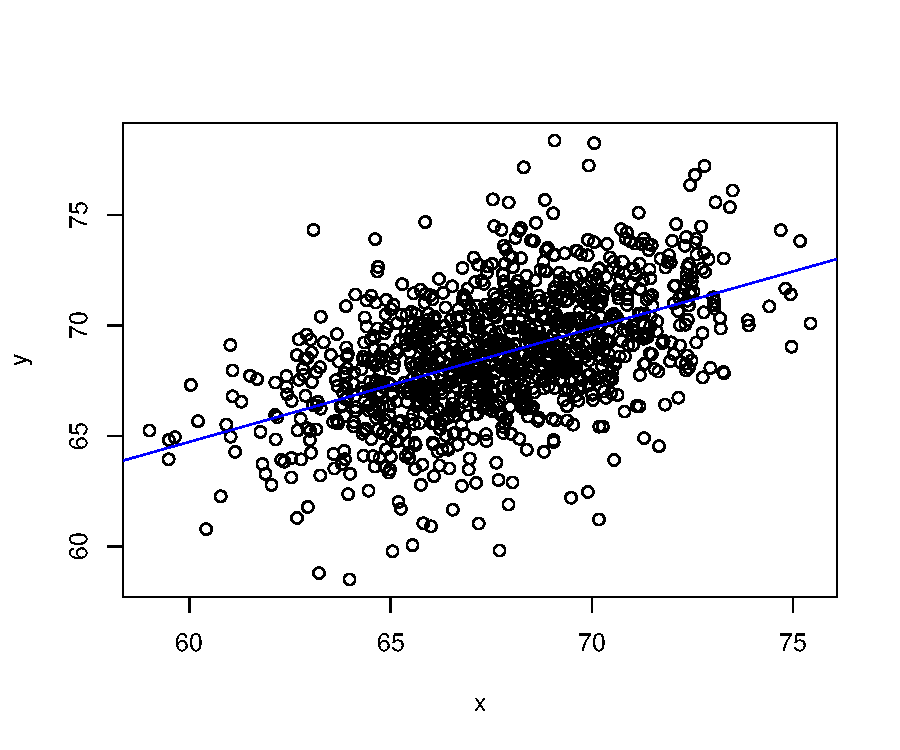
\includegraphics[keepaspectratio]{matrix_files/figure-pdf/unnamed-chunk-30-1.pdf}}
\end{center}

\subsection{Motivating Examples}\label{motivating-examples}

\paragraph{Falling objects}\label{falling-objects}

Imagine you are Galileo in the 16th century trying to describe the
velocity of a falling object. An assistant climbs the Tower of Pisa and
drops a ball, while several other assistants record the position at
different times. Let's simulate some data using the equations we know
today and adding some measurement error:

\begin{Shaded}
\begin{Highlighting}[]
\FunctionTok{set.seed}\NormalTok{(}\DecValTok{1}\NormalTok{)}
\NormalTok{g }\OtherTok{\textless{}{-}} \FloatTok{9.8} \DocumentationTok{\#\#meters per second}
\NormalTok{n }\OtherTok{\textless{}{-}} \DecValTok{25}
\NormalTok{tt }\OtherTok{\textless{}{-}} \FunctionTok{seq}\NormalTok{(}\DecValTok{0}\NormalTok{,}\FloatTok{3.4}\NormalTok{,}\AttributeTok{len=}\NormalTok{n) }\DocumentationTok{\#\#time in secs, note: we use tt because t is a base function}
\NormalTok{d }\OtherTok{\textless{}{-}} \FloatTok{56.67}  \SpecialCharTok{{-}} \FloatTok{0.5}\SpecialCharTok{*}\NormalTok{g}\SpecialCharTok{*}\NormalTok{tt}\SpecialCharTok{\^{}}\DecValTok{2} \SpecialCharTok{+} \FunctionTok{rnorm}\NormalTok{(n,}\AttributeTok{sd=}\DecValTok{1}\NormalTok{) }\DocumentationTok{\#\#meters}
\end{Highlighting}
\end{Shaded}

The assistants hand the data to Galileo and this is what he sees:

\begin{Shaded}
\begin{Highlighting}[]
\FunctionTok{mypar}\NormalTok{()}

\FunctionTok{plot}\NormalTok{(tt,d,}\AttributeTok{ylab=}\StringTok{"Distance in meters"}\NormalTok{,}\AttributeTok{xlab=}\StringTok{"Time in seconds"}\NormalTok{)}
\end{Highlighting}
\end{Shaded}

\begin{figure}[H]

{\centering \pandocbounded{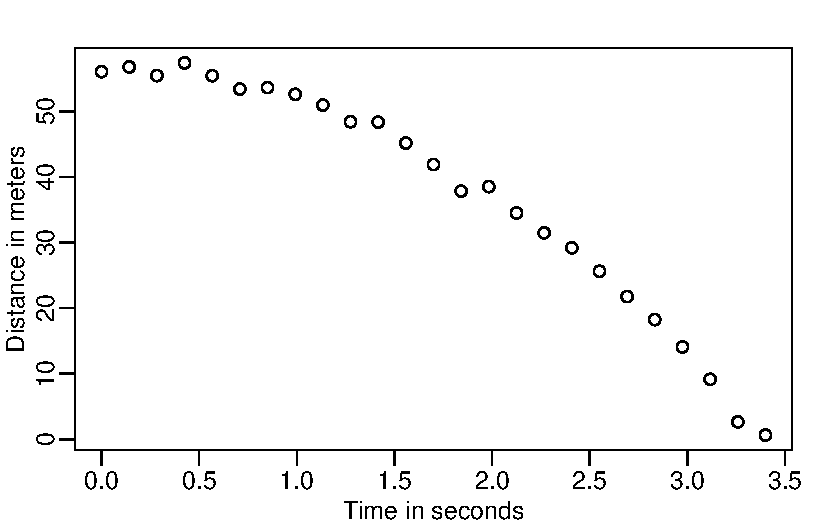
\includegraphics[keepaspectratio]{matrix_files/figure-pdf/gravity-1.pdf}}

}

\caption{Simulated data for distance travelled versus time of falling
object measured with error.}

\end{figure}%

He does not know the exact equation, but by looking at the plot above he
deduces that the position should follow a parabola. So he models the
data with:

\[ 
Y_i = \beta_0 + \beta_1 x_i + \beta_2 x_i^2 + \varepsilon_i, i=1,\dots,n 
\]

With \(Y_i\) representing location, \(x_i\) representing the time, and
\(\varepsilon_i\) accounting for measurement error. This is a linear
model because it is a linear combination of known quantities (the
\(x\)'s) referred to as predictors or covariates and unknown parameters
(the \(\beta\)'s).

so we are have our measures \texttt{d} and we want to calculate the
unknown parameters or betas: \texttt{h} is the hight of the Tower of
Pisa and should result in a value similar to 56.67 \texttt{g} is the
acceleration due to gravity, but we will actually get \(\frac{1}{2}g\)
due to physics. and we will have some errors due to measurament errors
that we introduced in the formula above using \texttt{rnorm(n,sd=1)}

we want to find the values of beta that minimize the sum square of
errors (RSS) Our first step is to create a matrix with tt and \(tt^2\)
and we add a column of 1s:

\begin{Shaded}
\begin{Highlighting}[]
\NormalTok{X}\OtherTok{\textless{}{-}} \FunctionTok{cbind}\NormalTok{(}\DecValTok{1}\NormalTok{,tt,tt}\SpecialCharTok{\^{}}\DecValTok{2}\NormalTok{)}
\NormalTok{X}
\end{Highlighting}
\end{Shaded}

\begin{verbatim}
               tt            
 [1,] 1 0.0000000  0.00000000
 [2,] 1 0.1416667  0.02006944
 [3,] 1 0.2833333  0.08027778
 [4,] 1 0.4250000  0.18062500
 [5,] 1 0.5666667  0.32111111
 [6,] 1 0.7083333  0.50173611
 [7,] 1 0.8500000  0.72250000
 [8,] 1 0.9916667  0.98340278
 [9,] 1 1.1333333  1.28444444
[10,] 1 1.2750000  1.62562500
[11,] 1 1.4166667  2.00694444
[12,] 1 1.5583333  2.42840278
[13,] 1 1.7000000  2.89000000
[14,] 1 1.8416667  3.39173611
[15,] 1 1.9833333  3.93361111
[16,] 1 2.1250000  4.51562500
[17,] 1 2.2666667  5.13777778
[18,] 1 2.4083333  5.80006944
[19,] 1 2.5500000  6.50250000
[20,] 1 2.6916667  7.24506944
[21,] 1 2.8333333  8.02777778
[22,] 1 2.9750000  8.85062500
[23,] 1 3.1166667  9.71361111
[24,] 1 3.2583333 10.61673611
[25,] 1 3.4000000 11.56000000
\end{verbatim}

Now we choose a random matrix for beta of 3 rows (so we can multiply by
X) Note that the values chosen for the matrix are arbitrary:

\begin{Shaded}
\begin{Highlighting}[]
\NormalTok{Beta }\OtherTok{\textless{}{-}} \FunctionTok{matrix}\NormalTok{(}\FunctionTok{c}\NormalTok{(}\DecValTok{55}\NormalTok{,}\DecValTok{0}\NormalTok{,}\DecValTok{5}\NormalTok{),}\DecValTok{3}\NormalTok{,}\DecValTok{1}\NormalTok{)}
\NormalTok{Beta}
\end{Highlighting}
\end{Shaded}

\begin{verbatim}
     [,1]
[1,]   55
[2,]    0
[3,]    5
\end{verbatim}

the residuals will be y - X times Beta.

\begin{Shaded}
\begin{Highlighting}[]
\NormalTok{r}\OtherTok{\textless{}{-}}\NormalTok{ d }\SpecialCharTok{{-}}\NormalTok{ X}\SpecialCharTok{\%*\%}\NormalTok{Beta}
\NormalTok{r}
\end{Highlighting}
\end{Shaded}

\begin{verbatim}
               [,1]
 [1,]    1.04354619
 [2,]    1.65495582
 [3,]    0.03962139
 [4,]    1.47709330
 [5,]   -1.17949223
 [6,]   -4.11765588
 [7,]   -4.99532095
 [8,]   -7.32736279
 [9,]  -10.47021865
[10,]  -14.72907589
[11,]  -16.68696883
[12,]  -21.98134426
[13,]  -27.56224058
[14,]  -34.12288739
[15,]  -36.14781908
[16,]  -43.07962111
[17,]  -49.21019026
[18,]  -54.80685129
[19,]  -61.88352880
[20,]  -69.46228618
[21,]  -76.88602263
[22,]  -85.16905120
[23,]  -94.42018502
[24,] -105.42503920
[25,] -112.15417425
\end{verbatim}

and the \emph{Residual Sum of Squares (RSS)} will be:

\begin{Shaded}
\begin{Highlighting}[]
\NormalTok{RSS}\OtherTok{\textless{}{-}} \FunctionTok{crossprod}\NormalTok{(r)}
\NormalTok{RSS}
\end{Highlighting}
\end{Shaded}

\begin{verbatim}
         [,1]
[1,] 66131.18
\end{verbatim}

now to get the values for our unknown parameters we solve the
\emph{least squares estimate (LSE)} for those

\begin{Shaded}
\begin{Highlighting}[]
\NormalTok{betahat }\OtherTok{\textless{}{-}} \FunctionTok{solve}\NormalTok{(}\FunctionTok{crossprod}\NormalTok{(X))}\SpecialCharTok{\%*\%} \FunctionTok{crossprod}\NormalTok{(X,d)}
\NormalTok{betahat}
\end{Highlighting}
\end{Shaded}

\begin{verbatim}
         [,1]
   56.5317368
tt  0.5013565
   -5.0386455
\end{verbatim}

which gives us: 57.0212322 is the hight of the tower of Pisa -0.4223921
is the starting velocity (should be 0) -4.8175119 is half of the gravity
acceleration.

which will result in our formula:
\texttt{d\ \textless{}-\ 57.0212322\ -\ 0.4223921\ tt\ -\ 4.8175119\ tt\^{}2}

\begin{Shaded}
\begin{Highlighting}[]
\NormalTok{fun }\OtherTok{\textless{}{-}} \ControlFlowTok{function}\NormalTok{(x)\{}
  \FloatTok{57.0212322} \SpecialCharTok{{-}}\NormalTok{ (}\FloatTok{0.4223921}\SpecialCharTok{*}\NormalTok{x) }\SpecialCharTok{{-}}\NormalTok{ (}\FloatTok{4.8175119}\SpecialCharTok{*}\NormalTok{x}\SpecialCharTok{\^{}}\DecValTok{2}\NormalTok{)\}}
\NormalTok{y\_1 }\OtherTok{\textless{}{-}} \FunctionTok{fun}\NormalTok{(tt)}
\end{Highlighting}
\end{Shaded}

Now we can plot the measured values along with the calculated values
using the equation (note that I have slightly displaced the calculated
values to avoid overlapping)

\begin{Shaded}
\begin{Highlighting}[]
\CommentTok{\# Plot the measured values}
\FunctionTok{plot}\NormalTok{(tt, d, }\AttributeTok{xlab =} \StringTok{"Time in secs"}\NormalTok{, }\AttributeTok{ylab =} \StringTok{"Distance in m."}\NormalTok{, }\AttributeTok{col =} \StringTok{"blue"}\NormalTok{, }\AttributeTok{pch =} \DecValTok{19}\NormalTok{)}

\CommentTok{\# Add the fitted values to the plot}
\FunctionTok{points}\NormalTok{(tt}\FloatTok{+0.1}\NormalTok{, y\_1, }\AttributeTok{col =} \StringTok{"red"}\NormalTok{, }\AttributeTok{pch =} \DecValTok{17}\NormalTok{)}

\CommentTok{\# Add a legend to differentiate between the two lines}
\FunctionTok{legend}\NormalTok{(}\StringTok{"bottomleft"}\NormalTok{, }\AttributeTok{legend =} \FunctionTok{c}\NormalTok{(}\StringTok{"Measured values"}\NormalTok{, }\StringTok{"Fitted values"}\NormalTok{), }\AttributeTok{col =} \FunctionTok{c}\NormalTok{(}\StringTok{"blue"}\NormalTok{, }\StringTok{"red"}\NormalTok{), }\AttributeTok{pch =} \FunctionTok{c}\NormalTok{(}\DecValTok{19}\NormalTok{, }\DecValTok{17}\NormalTok{))}
\end{Highlighting}
\end{Shaded}

\begin{center}
\pandocbounded{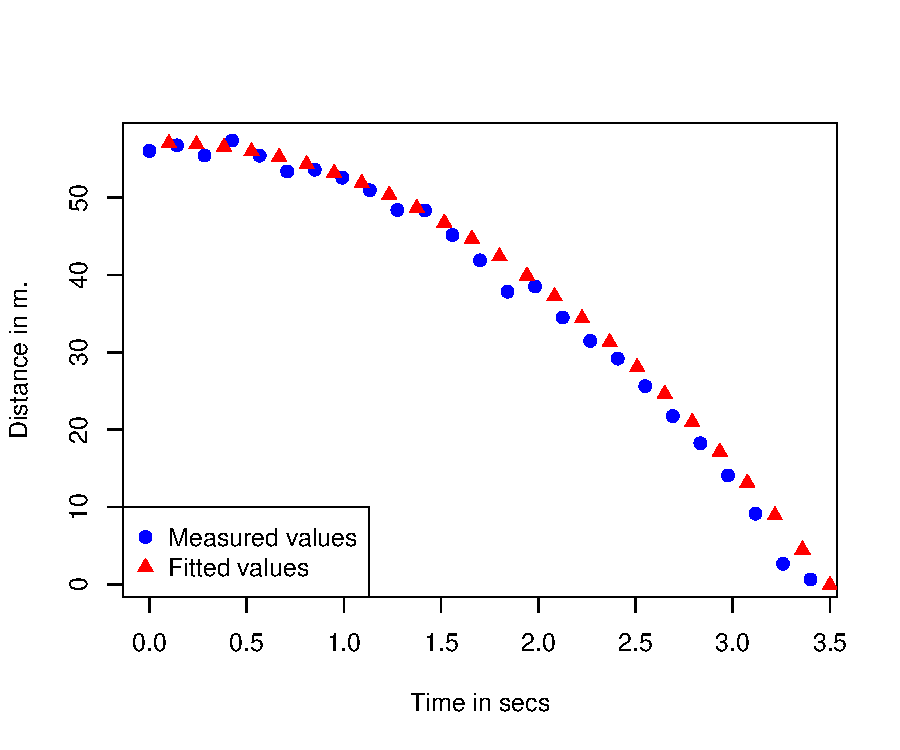
\includegraphics[keepaspectratio]{matrix_files/figure-pdf/unnamed-chunk-38-1.pdf}}
\end{center}

We could have solved this without matrices using the linear model
formula in r:

\begin{Shaded}
\begin{Highlighting}[]
\NormalTok{tt2}\OtherTok{\textless{}{-}}\NormalTok{ tt}\SpecialCharTok{\^{}}\DecValTok{2}
\NormalTok{fit }\OtherTok{\textless{}{-}} \FunctionTok{lm}\NormalTok{(d}\SpecialCharTok{\textasciitilde{}}\NormalTok{tt}\SpecialCharTok{+}\NormalTok{tt2)}
\FunctionTok{summary}\NormalTok{(fit)}
\end{Highlighting}
\end{Shaded}

\begin{verbatim}

Call:
lm(formula = d ~ tt + tt2)

Residuals:
    Min      1Q  Median      3Q     Max 
-2.5295 -0.4882  0.2537  0.6560  1.5455 

Coefficients:
            Estimate Std. Error t value            Pr(>|t|)    
(Intercept)  56.5317     0.5451 103.701 <0.0000000000000002 ***
tt            0.5014     0.7426   0.675               0.507    
tt2          -5.0386     0.2110 -23.884 <0.0000000000000002 ***
---
Signif. codes:  0 '***' 0.001 '**' 0.01 '*' 0.05 '.' 0.1 ' ' 1

Residual standard error: 0.9822 on 22 degrees of freedom
Multiple R-squared:  0.9973,    Adjusted R-squared:  0.997 
F-statistic:  4025 on 2 and 22 DF,  p-value: < 0.00000000000000022
\end{verbatim}

\subsection{Standard Error in the context of linear
models}\label{standard-error-in-the-context-of-linear-models}

We have shown how to find the least squares estimates with matrix
algebra. These estimates are random variables as they are linear
combinations of the data. For these estimates to be useful we also need
to compute the standard errors.

It is useful to think about where randomness comes from. In our falling
object example, randomness was introduced through measurement errors.
Every time we rerun the experiment a new set of measurement errors will
be made which implies our data will be random. This implies that our
estimate of the gravitational constant will change. The constant is
fixed, but our estimates are not. To see this we can run a Monte Carlo
simulation. Specifically we will generate the data repeatedly and
compute the estimate for the quadratic term each time.

\begin{Shaded}
\begin{Highlighting}[]
\NormalTok{g }\OtherTok{=} \FloatTok{9.8} \DocumentationTok{\#\# meters per second}
\NormalTok{h0 }\OtherTok{=} \FloatTok{56.67}
\NormalTok{v0 }\OtherTok{=} \DecValTok{0}
\NormalTok{n }\OtherTok{=} \DecValTok{25}
\NormalTok{tt }\OtherTok{=} \FunctionTok{seq}\NormalTok{(}\DecValTok{0}\NormalTok{,}\FloatTok{3.4}\NormalTok{,}\AttributeTok{len=}\NormalTok{n) }\DocumentationTok{\#\#time in secs, t is a base function}
\NormalTok{y }\OtherTok{=}\NormalTok{ h0 }\SpecialCharTok{+}\NormalTok{ v0 }\SpecialCharTok{*}\NormalTok{tt  }\SpecialCharTok{{-}} \FloatTok{0.5}\SpecialCharTok{*}\NormalTok{ g}\SpecialCharTok{*}\NormalTok{tt}\SpecialCharTok{\^{}}\DecValTok{2} \SpecialCharTok{+} \FunctionTok{rnorm}\NormalTok{(n,}\AttributeTok{sd=}\DecValTok{1}\NormalTok{)}
\end{Highlighting}
\end{Shaded}

now we act as if we didn't know \texttt{h0}, \texttt{v0} and
\texttt{-0.5g} and use regression to estimate these. We can rewrite the
models as \texttt{y=b0+b1\ t+\ b2\ t\^{}2\ +e} and obtain LSE. Note that
g will be \texttt{g=-2*b2}

To obtain the LSE in r

\begin{Shaded}
\begin{Highlighting}[]
\NormalTok{X }\OtherTok{=} \FunctionTok{cbind}\NormalTok{(}\DecValTok{1}\NormalTok{,tt,tt}\SpecialCharTok{\^{}}\DecValTok{2}\NormalTok{)}
\NormalTok{A }\OtherTok{=} \FunctionTok{solve}\NormalTok{(}\FunctionTok{crossprod}\NormalTok{(X))}\SpecialCharTok{\%*\%}\FunctionTok{t}\NormalTok{(X)}\SpecialCharTok{\%*\%}\NormalTok{y}
\end{Highlighting}
\end{Shaded}

so g will be measured after this experiment as:

\begin{Shaded}
\begin{Highlighting}[]
\SpecialCharTok{{-}}\DecValTok{2}\SpecialCharTok{*}\NormalTok{A[}\DecValTok{3}\NormalTok{]}
\end{Highlighting}
\end{Shaded}

\begin{verbatim}
[1] 9.788724
\end{verbatim}

now we are going to repeat the experiment 100,000 times and calculate
the standard deviation for the estimate g.

\begin{Shaded}
\begin{Highlighting}[]
\NormalTok{g }\OtherTok{=} \FloatTok{9.8} \DocumentationTok{\#\# meters per second}
\NormalTok{h0 }\OtherTok{=} \FloatTok{56.67}
\NormalTok{v0 }\OtherTok{=} \DecValTok{0}
\NormalTok{n }\OtherTok{=} \DecValTok{25}
\NormalTok{tt }\OtherTok{=} \FunctionTok{seq}\NormalTok{(}\DecValTok{0}\NormalTok{,}\FloatTok{3.4}\NormalTok{,}\AttributeTok{len=}\NormalTok{n) }\DocumentationTok{\#\#time in secs, t is a base function}
\FunctionTok{set.seed}\NormalTok{(}\DecValTok{1}\NormalTok{)}
\NormalTok{myfunc }\OtherTok{\textless{}{-}} \ControlFlowTok{function}\NormalTok{()\{}
\NormalTok{y }\OtherTok{=}\NormalTok{ h0 }\SpecialCharTok{+}\NormalTok{ v0 }\SpecialCharTok{*}\NormalTok{tt  }\SpecialCharTok{{-}} \FloatTok{0.5}\SpecialCharTok{*}\NormalTok{ g}\SpecialCharTok{*}\NormalTok{tt}\SpecialCharTok{\^{}}\DecValTok{2} \SpecialCharTok{+} \FunctionTok{rnorm}\NormalTok{(n,}\AttributeTok{sd=}\DecValTok{1}\NormalTok{)}

\NormalTok{X }\OtherTok{=} \FunctionTok{cbind}\NormalTok{(}\DecValTok{1}\NormalTok{,tt,tt}\SpecialCharTok{\^{}}\DecValTok{2}\NormalTok{)}
\NormalTok{A }\OtherTok{=} \FunctionTok{solve}\NormalTok{(}\FunctionTok{crossprod}\NormalTok{(X))}\SpecialCharTok{\%*\%}\FunctionTok{t}\NormalTok{(X)}\SpecialCharTok{\%*\%}\NormalTok{y}
\NormalTok{A}
\NormalTok{g}\OtherTok{\textless{}{-}} \SpecialCharTok{{-}}\DecValTok{2}\SpecialCharTok{*}\NormalTok{A[}\DecValTok{3}\NormalTok{]}
\FunctionTok{return}\NormalTok{ (g)}
\NormalTok{\}}

\NormalTok{gs}\OtherTok{\textless{}{-}} \FunctionTok{replicate}\NormalTok{(}\DecValTok{100000}\NormalTok{,}\FunctionTok{myfunc}\NormalTok{())}
\FunctionTok{sd}\NormalTok{(gs)}
\end{Highlighting}
\end{Shaded}

\begin{verbatim}
[1] 0.429747
\end{verbatim}

Now we are going to use matrix algebra to compute standard errors of
regression coefficients. We will start by defining the \emph{variance
covariance matrix}.

\subsubsection{Variance-covariance matrix
(Advanced)}\label{variance-covariance-matrix-advanced}

As a first step we need to define the \emph{variance-covariance matrix},
\(\boldsymbol{\Sigma}\). For a vector of random variables,
\(\mathbf{Y}\), we define \(\boldsymbol{\Sigma}\) as the matrix with the
\(i,j\) entry:

\[ \Sigma_{i,j} \equiv \mbox{Cov}(Y_i, Y_j) \] The covariance is equal
to the variance if \(i = j\) and equal to 0 if the variables are
independent. In the kinds of vectors considered up to now, for example,
a vector \(\mathbf{Y}\) of individual observations \(Y_i\) sampled from
a population, we have assumed independence of each observation and
assumed the \(Y_i\) all have the same variance \(\sigma^2\), so the
variance-covariance matrix has had only two kinds of elements:

\[ \mbox{Cov}(Y_i, Y_i) = \mbox{var}(Y_i) = \sigma^2\]

\[ \mbox{Cov}(Y_i, Y_j) = 0, \mbox{ for } i \neq j\]

which implies that \(\boldsymbol{\Sigma} = \sigma^2 \mathbf{I}\) with
\(\mathbf{I}\), the identity matrix.

Later, we will see a case, specifically the estimate coefficients of a
linear model, \(\hat{\boldsymbol{\beta}}\), that has non-zero entries in
the off diagonal elements of \(\boldsymbol{\Sigma}\). Furthermore, the
diagonal elements will not be equal to a single value \(\sigma^2\).

\subsubsection{Variance of a linear
combination}\label{variance-of-a-linear-combination}

A useful result provided by linear algebra is that the variance
covariance-matrix of a linear combination \(\mathbf{AY}\) of
\(\mathbf{Y}\) can be computed as follows:

\[
\mbox{var}(\mathbf{AY}) = \mathbf{A}\mbox{var}(\mathbf{Y}) \mathbf{A}^\top 
\]

For example, if \(Y_1\) and \(Y_2\) are independent both with variance
\(\sigma^2\) then:

\[\mbox{var}\{Y_1+Y_2\} = 
\mbox{var}\left\{ \begin{pmatrix}1&1\end{pmatrix}\begin{pmatrix} Y_1\\Y_2\\ \end{pmatrix}\right\}\]

\[ =\begin{pmatrix}1&1\end{pmatrix} \sigma^2 \mathbf{I}\begin{pmatrix} 1\\1\\ \end{pmatrix}=2\sigma^2\]

as we expect. We use this result to obtain the standard errors of the
LSE (least squares estimate).

\subsection{Least Squares Estimates (LSE) standard errors
(Advanced)}\label{least-squares-estimates-lse-standard-errors-advanced}

Note that the LSE \(\boldsymbol{\hat{\beta}}\) is a linear combination
of \(\mathbf{Y}\): \(\mathbf{AY}\) with
\(\mathbf{A}=\mathbf{(X^\top X)^{-1}X}^\top\), so we can use the
equation above to derive the variance of our estimates:

\[\mbox{var}(\boldsymbol{\hat{\beta}}) = \mbox{var}(\mathbf{(X^\top X)^{-1}X^\top Y}) =  \]

\[\mathbf{(X^\top X)^{-1} X^\top} \mbox{var}(Y) (\mathbf{(X^\top X)^{-1} X^\top})^\top = \]

\[\mathbf{(X^\top X)^{-1} X^\top} \sigma^2 \mathbf{I} (\mathbf{(X^\top X)^{-1} X^\top})^\top = \]

\[\sigma^2 \mathbf{(X^\top X)^{-1} X^\top}\mathbf{X} \mathbf{(X^\top X)^{-1}} = \]

\[\sigma^2\mathbf{(X^\top X)^{-1}}\]

The diagonal of the square root of this matrix contains the standard
error of our estimates.

\paragraph{\texorpdfstring{Estimating
\(\sigma^2\)}{Estimating \textbackslash sigma\^{}2}}\label{estimating-sigma2}

To obtain an actual estimate in practice from the formulas above, we
need to estimate \(\sigma^2\). Previously we estimated the standard
errors from the sample. However, the sample standard deviation of \(Y\)
is not \(\sigma\) because \(Y\) also includes variability introduced by
the deterministic part of the model: \(\mathbf{X}\boldsymbol{\beta}\).
The approach we take is to use the residuals.

We form the residuals like this:

\[
\mathbf{r}\equiv\boldsymbol{\hat{\varepsilon}} = \mathbf{Y}-\mathbf{X}\boldsymbol{\hat{\beta}}
\]

Both \(\mathbf{r}\) and \(\boldsymbol{\hat{\varepsilon}}\) notations are
used to denote residuals.

Then we use these to estimate, in a similar way, to what we do in the
univariate case:

\[ s^2 \equiv \hat{\sigma}^2 = \frac{1}{N-p}\mathbf{r}^\top\mathbf{r} = \frac{1}{N-p}\sum_{i=1}^N r_i^2\]

Here \(N\) is the sample size and \(p\) is the number of columns in
\(\mathbf{X}\) or number of parameters (including the intercept term
\(\beta_0\)). The reason we divide by \(N-p\) is because mathematical
theory tells us that this will give us a better (unbiased) estimate.

Let's try this in R and see if we obtain the same values as we did with
the Monte Carlo simulation above:

\begin{Shaded}
\begin{Highlighting}[]
\NormalTok{n }\OtherTok{\textless{}{-}} \FunctionTok{nrow}\NormalTok{(father.son)}
\NormalTok{N }\OtherTok{\textless{}{-}} \DecValTok{50}
\NormalTok{index }\OtherTok{\textless{}{-}} \FunctionTok{sample}\NormalTok{(n,N)}
\NormalTok{sampledat }\OtherTok{\textless{}{-}}\NormalTok{ father.son[index,]}
\NormalTok{x }\OtherTok{\textless{}{-}}\NormalTok{ sampledat}\SpecialCharTok{$}\NormalTok{fheight}
\NormalTok{y }\OtherTok{\textless{}{-}}\NormalTok{ sampledat}\SpecialCharTok{$}\NormalTok{sheight}
\NormalTok{X }\OtherTok{\textless{}{-}} \FunctionTok{model.matrix}\NormalTok{(}\SpecialCharTok{\textasciitilde{}}\NormalTok{x)}

\NormalTok{N }\OtherTok{\textless{}{-}} \FunctionTok{nrow}\NormalTok{(X)}
\NormalTok{p }\OtherTok{\textless{}{-}} \FunctionTok{ncol}\NormalTok{(X)}

\NormalTok{XtXinv }\OtherTok{\textless{}{-}} \FunctionTok{solve}\NormalTok{(}\FunctionTok{crossprod}\NormalTok{(X))}

\NormalTok{resid }\OtherTok{\textless{}{-}}\NormalTok{ y }\SpecialCharTok{{-}}\NormalTok{ X }\SpecialCharTok{\%*\%}\NormalTok{ XtXinv }\SpecialCharTok{\%*\%} \FunctionTok{crossprod}\NormalTok{(X,y)}

\NormalTok{s }\OtherTok{\textless{}{-}} \FunctionTok{sqrt}\NormalTok{(}\FunctionTok{sum}\NormalTok{(resid}\SpecialCharTok{\^{}}\DecValTok{2}\NormalTok{)}\SpecialCharTok{/}\NormalTok{(N}\SpecialCharTok{{-}}\NormalTok{p))}
\NormalTok{ses }\OtherTok{\textless{}{-}} \FunctionTok{sqrt}\NormalTok{(}\FunctionTok{diag}\NormalTok{(XtXinv))}\SpecialCharTok{*}\NormalTok{s }
\end{Highlighting}
\end{Shaded}

Let's compare to what \texttt{lm} provides:

\begin{Shaded}
\begin{Highlighting}[]
\FunctionTok{summary}\NormalTok{(}\FunctionTok{lm}\NormalTok{(y}\SpecialCharTok{\textasciitilde{}}\NormalTok{x))}\SpecialCharTok{$}\NormalTok{coef[,}\DecValTok{2}\NormalTok{]}
\end{Highlighting}
\end{Shaded}

\begin{verbatim}
(Intercept)           x 
  8.7487832   0.1284109 
\end{verbatim}

\begin{Shaded}
\begin{Highlighting}[]
\NormalTok{ses}
\end{Highlighting}
\end{Shaded}

\begin{verbatim}
(Intercept)           x 
  8.7487832   0.1284109 
\end{verbatim}

They are identical because they are doing the same thing. Also, note
that we approximate the Monte Carlo results:

\begin{Shaded}
\begin{Highlighting}[]
\FunctionTok{apply}\NormalTok{(betahat,}\DecValTok{2}\NormalTok{,sd)}
\end{Highlighting}
\end{Shaded}

\begin{verbatim}
[1] 34.06124
\end{verbatim}

\subsection{Linear combination of
estimates}\label{linear-combination-of-estimates}

Imagine that you estimated the effects of several treatments and now you
are interested in the difference in the effects of two of those
treatments. You already have the \(\hat{\beta}\) and want to calculate
\(\hat{\beta}_2-\hat{\beta}_1\)

If we want to compute the standard deviation of a linear combination of
estimates such as \(\hat{\beta}_2 - \hat{\beta}_1\), this is a linear
combination of \(\hat{\boldsymbol{\beta}}\):

\[\hat{\beta}_2 - \hat{\beta}_1 = 
\begin{pmatrix}0&-1&1&0&\dots&0\end{pmatrix} \begin{pmatrix}
\hat{\beta}_0\\
\hat{\beta}_1 \\ 
\hat{\beta}_2 \\ 
\vdots\\
\hat{\beta}_p
\end{pmatrix}\]

Using the above, we know how to compute the variance covariance matrix
of \(\hat{\boldsymbol{\beta}}\).

\subsection{CLT and t-distribution}\label{clt-and-t-distribution}

We have shown how we can obtain standard errors for our estimates.
However, as we learned in the first chapter, to perform inference we
need to know the distribution of these random variables. The reason we
went through the effort to compute the standard errors is because the
CLT applies in linear models. If \(N\) is large enough, then the LSE
will be normally distributed with mean \(\boldsymbol{\beta}\) and
standard errors as described. For small samples, if the \(\varepsilon\)
are normally distributed, then the \(\hat{\beta}-\beta\) follow a
t-distribution. We do not derive this result here, but the results are
extremely useful since it is how we construct p-values and confidence
intervals in the context of linear models.

\paragraph{Code versus math}\label{code-versus-math}

The standard approach to writing linear models either assume the values
in \(\mathbf{X}\) are fixed or that we are conditioning on them. Thus
\(\mathbf{X} \boldsymbol{\beta}\) has no variance as the \(\mathbf{X}\)
is considered fixed. This is why we write
\(\mbox{var}(Y_i) = \mbox{var}(\varepsilon_i)=\sigma^2\). This can cause
confusion in practice because if you, for example, compute the
following:

\begin{Shaded}
\begin{Highlighting}[]
\NormalTok{x }\OtherTok{=}\NormalTok{  father.son}\SpecialCharTok{$}\NormalTok{fheight}
\NormalTok{beta }\OtherTok{=}  \FunctionTok{c}\NormalTok{(}\DecValTok{34}\NormalTok{,}\FloatTok{0.5}\NormalTok{)}
\FunctionTok{var}\NormalTok{(beta[}\DecValTok{1}\NormalTok{]}\SpecialCharTok{+}\NormalTok{beta[}\DecValTok{2}\NormalTok{]}\SpecialCharTok{*}\NormalTok{x)}
\end{Highlighting}
\end{Shaded}

\begin{verbatim}
[1] 1.883576
\end{verbatim}

it is nowhere near 0. This is an example in which we have to be careful
in distinguishing code from math. The function \texttt{var} is simply
computing the variance of the list we feed it, while the mathematical
definition of variance is considering only quantities that are random
variables. In the R code above, \texttt{x} is not fixed at all: we are
letting it vary, but when we write \(\mbox{var}(Y_i) = \sigma^2\) we are
imposing, mathematically, \texttt{x} to be fixed. Similarly, if we use R
to compute the variance of \(Y\) in our object dropping example, we
obtain something very different than \(\sigma^2=1\) (the known
variance):

\begin{Shaded}
\begin{Highlighting}[]
\NormalTok{n }\OtherTok{\textless{}{-}} \FunctionTok{length}\NormalTok{(tt)}
\NormalTok{y }\OtherTok{\textless{}{-}}\NormalTok{ h0 }\SpecialCharTok{+}\NormalTok{ v0}\SpecialCharTok{*}\NormalTok{tt  }\SpecialCharTok{{-}} \FloatTok{0.5}\SpecialCharTok{*}\NormalTok{g}\SpecialCharTok{*}\NormalTok{tt}\SpecialCharTok{\^{}}\DecValTok{2} \SpecialCharTok{+} \FunctionTok{rnorm}\NormalTok{(n,}\AttributeTok{sd=}\DecValTok{1}\NormalTok{)}
\FunctionTok{var}\NormalTok{(y)}
\end{Highlighting}
\end{Shaded}

\begin{verbatim}
[1] 334.0487
\end{verbatim}

Again, this is because we are not fixing \texttt{tt}.

\paragraph{Exercise}\label{exercise}

We are going to calculate the standard error of \(\hat{\beta}\) for the
heights of father and son. \[
SE(\hat{\beta})= sqrt{Var(\hat{\beta})}
\]

\[
Var(\hat{\beta})= \sigma^2(X^TX)^{-1}
\]

First, we want to estimate \(\sigma^2\), the variance of Y. As we have
seen in the previous unit, the random part of Y is only coming from
\(\epsilon\), because we assume \(X\beta\) is fixed. So we can try to
estimate the variance of the epsilons from the residuals: the Y minus
the fitted values from the linear model.

\begin{Shaded}
\begin{Highlighting}[]
\NormalTok{x }\OtherTok{=}\NormalTok{ father.son}\SpecialCharTok{$}\NormalTok{fheight}
\NormalTok{y }\OtherTok{=}\NormalTok{ father.son}\SpecialCharTok{$}\NormalTok{sheight}
\NormalTok{n }\OtherTok{=} \FunctionTok{length}\NormalTok{(y)}
\NormalTok{N }\OtherTok{=} \DecValTok{50}
\FunctionTok{set.seed}\NormalTok{(}\DecValTok{1}\NormalTok{)}
\NormalTok{index }\OtherTok{=} \FunctionTok{sample}\NormalTok{(n,N)}
\NormalTok{sampledat }\OtherTok{=}\NormalTok{ father.son[index,]}
\NormalTok{x }\OtherTok{=}\NormalTok{ sampledat}\SpecialCharTok{$}\NormalTok{fheight}
\NormalTok{y }\OtherTok{=}\NormalTok{ sampledat}\SpecialCharTok{$}\NormalTok{sheight}
\NormalTok{betahat }\OtherTok{=} \FunctionTok{lm}\NormalTok{(y}\SpecialCharTok{\textasciitilde{}}\NormalTok{x)}\SpecialCharTok{$}\NormalTok{coef}
\end{Highlighting}
\end{Shaded}

first we calculate the \(\hat{Y}\) values from a linear model:

\begin{Shaded}
\begin{Highlighting}[]
\NormalTok{fit }\OtherTok{=} \FunctionTok{lm}\NormalTok{(y }\SpecialCharTok{\textasciitilde{}}\NormalTok{ x)}
\NormalTok{Yhat}\OtherTok{\textless{}{-}}\NormalTok{ fit}\SpecialCharTok{$}\NormalTok{fitted.values}
\end{Highlighting}
\end{Shaded}

and now we can calculate the sum of the squares residuals SSR that will
be the diffeence between \(y_i\) and \(\hat{y_i}\)

\begin{Shaded}
\begin{Highlighting}[]
\NormalTok{res2 }\OtherTok{\textless{}{-}}\NormalTok{ (y}\SpecialCharTok{{-}}\NormalTok{ Yhat)}\SpecialCharTok{\^{}}\DecValTok{2}
\NormalTok{SSR }\OtherTok{\textless{}{-}} \FunctionTok{sum}\NormalTok{(res2)}
\NormalTok{SSR}
\end{Highlighting}
\end{Shaded}

\begin{verbatim}
[1] 331.2952
\end{verbatim}

Our estimate of \(\sigma^2\) will be the sum of squared residuals
divided by (N-p), the sample size minus the number of terms in the
model. Since we have a sample of 50 and 2 terms in the model (the
intercept and a slope), our estimate will be:

\begin{Shaded}
\begin{Highlighting}[]
\NormalTok{sigma2 }\OtherTok{\textless{}{-}}\NormalTok{ SSR}\SpecialCharTok{/}\NormalTok{(N}\DecValTok{{-}2}\NormalTok{)}
\NormalTok{sigma2}
\end{Highlighting}
\end{Shaded}

\begin{verbatim}
[1] 6.901984
\end{verbatim}

Now we form the matrix X, this can be done by combining a column of 1s
with a column with the father's heights.

\begin{Shaded}
\begin{Highlighting}[]
\NormalTok{X }\OtherTok{=} \FunctionTok{cbind}\NormalTok{(}\FunctionTok{rep}\NormalTok{(}\DecValTok{1}\NormalTok{,N),x)}
\end{Highlighting}
\end{Shaded}

And now we calculate \((X^TX)^{-1}\)

\begin{Shaded}
\begin{Highlighting}[]
\NormalTok{I}\OtherTok{\textless{}{-}}\FunctionTok{solve}\NormalTok{(}\FunctionTok{t}\NormalTok{(X)}\SpecialCharTok{\%*\%}\NormalTok{X)}
\NormalTok{I}
\end{Highlighting}
\end{Shaded}

\begin{verbatim}
                        x
  14.5639039 -0.214704345
x -0.2147043  0.003169572
\end{verbatim}

Now we are only one step away from getting the standard error of
\(\hat{\beta}\) Take the diagonals of \((X^TX)^{-1}\) and multiply by
our estimate of \(\sigma^2\). This is the estimated variance of
\(\hat{\beta}\)

\begin{Shaded}
\begin{Highlighting}[]
\NormalTok{varianceBeta }\OtherTok{\textless{}{-}} \FunctionTok{diag}\NormalTok{(I)}\SpecialCharTok{*}\NormalTok{sigma2}
\NormalTok{varianceBeta}
\end{Highlighting}
\end{Shaded}

\begin{verbatim}
                        x 
100.51983131   0.02187634 
\end{verbatim}

and finally the SE will be the square root of this

\begin{Shaded}
\begin{Highlighting}[]
\NormalTok{SE}\OtherTok{\textless{}{-}} \FunctionTok{sqrt}\NormalTok{(varianceBeta)}
\NormalTok{SE}
\end{Highlighting}
\end{Shaded}

\begin{verbatim}
                    x 
10.0259579  0.1479065 
\end{verbatim}

this gives us two numbers, the standard error of the intercept and the
standard error for the slope. (Note that the standard error estimate is
also printed int eh second column of \texttt{summary(fit)})

\begin{Shaded}
\begin{Highlighting}[]
\FunctionTok{summary}\NormalTok{(fit)}
\end{Highlighting}
\end{Shaded}

\begin{verbatim}

Call:
lm(formula = y ~ x)

Residuals:
    Min      1Q  Median      3Q     Max 
-7.8912 -1.3527  0.3593  1.5703  4.4794 

Coefficients:
            Estimate Std. Error t value  Pr(>|t|)    
(Intercept)  44.3377    10.0260   4.422 0.0000558 ***
x             0.3530     0.1479   2.387     0.021 *  
---
Signif. codes:  0 '***' 0.001 '**' 0.01 '*' 0.05 '.' 0.1 ' ' 1

Residual standard error: 2.627 on 48 degrees of freedom
Multiple R-squared:  0.1061,    Adjusted R-squared:  0.08747 
F-statistic: 5.697 on 1 and 48 DF,  p-value: 0.02098
\end{verbatim}

\section{Linear models as matrix
multiplication.}\label{linear-models-as-matrix-multiplication.}

Suppose we have a linear model with 4 variables \[ 
Y_i = \beta_0 + \beta_1 X_{i1} + \beta_2 X_{i2} + \beta_3 X_{i3} + \beta_4 X_{i4} + \epsilon_i
\] that can be written as: \[ 
\mathbf{Y} = \mathbf{X} \boldsymbol{\beta} + \boldsymbol{\epsilon} 
\]

where

\[ 
\mathbf{Y} =
\begin{pmatrix} 
Y_1 \\ 
Y_2 \\ 
\vdots \\
\ Y_N 
\end{pmatrix}
\]

\[ 
\mathbf{X} =
\begin{pmatrix}
1 & X_{11} & X_{12} & X_{13} & X_{14} \\
1 & X_{21} & X_{22} & X_{23} & X_{24} \\
\vdots & \vdots & \vdots & \vdots & \vdots \\
1 & X_{N1} & X_{N2} & X_{N3} & X_{N4}
\end{pmatrix}
\]

\[ 
\boldsymbol{\beta} =
\begin{pmatrix} 
\beta_0 \\ 
\beta_1 \\ 
\beta_2 \\ 
\beta_3 \\ 
\beta_4 
\end{pmatrix}
\] and \[ 
\boldsymbol{\epsilon} =
\begin{pmatrix}
\epsilon_1 \\
\epsilon_2 \\
\vdots \\
\epsilon_N
\end{pmatrix}
\]

\[
\begin{bmatrix}
Y_1 \\
Y_2 \\
Y_3 \\
Y_4 \\
Y_5 \\
Y_6
\end{bmatrix}
=
\begin{bmatrix}
1 & X_{11} & X_{12} & X_{13} & X_{14} \\
1 & X_{21} & X_{22} & X_{23} & X_{24} \\
1 & X_{31} & X_{32} & X_{33} & X_{34} \\
1 & X_{41} & X_{42} & X_{43} & X_{44} \\
1 & X_{51} & X_{52} & X_{53} & X_{54} \\
1 & X_{61} & X_{62} & X_{63} & X_{64}
\end{bmatrix}
\begin{bmatrix}
\beta_0 \\
\beta_1 \\
\beta_2 \\
\beta_3 \\
\beta_4
\end{bmatrix}
+
\begin{bmatrix}
\epsilon_1 \\
\epsilon_2 \\
\epsilon_3 \\
\epsilon_4 \\
\epsilon_5 \\
\epsilon_6
\end{bmatrix}
\]

the sum of least squares will be:

\[ 
\sum_{i=1}^{N} \left(Y_i - \beta_0 - \beta_1 X_{i1} - \beta_2 X_{i2} - \beta_3 X_{i3} - \beta_4 X_{i4}\right)^2
\] in matrix notation that would be \[
(Y-\beta X)^T(Y-\beta X) 
\]

\section{t-test}\label{t-test}

When we are doing a t-test we calculate the average in one group and
substract from the average in the other group and that is an estimate of
the population average.

We are going to make something difference. We will get a baseline,
\(\hat{\beta_0}\) and we are going to calculate the difference between
the two groups \(\hat{\beta_1}\)

\begin{Shaded}
\begin{Highlighting}[]
\FunctionTok{set.seed}\NormalTok{(}\DecValTok{123}\NormalTok{)}

\CommentTok{\# Generate data for two groups}
\NormalTok{group }\OtherTok{\textless{}{-}} \FunctionTok{rep}\NormalTok{(}\FunctionTok{c}\NormalTok{(}\StringTok{"A"}\NormalTok{, }\StringTok{"B"}\NormalTok{), }\AttributeTok{each =} \DecValTok{20}\NormalTok{)}
\NormalTok{x }\OtherTok{\textless{}{-}} \FunctionTok{c}\NormalTok{(}\FunctionTok{rnorm}\NormalTok{(}\DecValTok{20}\NormalTok{, }\AttributeTok{mean =} \DecValTok{1}\NormalTok{, }\AttributeTok{sd =} \FloatTok{0.5}\NormalTok{), }\FunctionTok{rnorm}\NormalTok{(}\DecValTok{20}\NormalTok{, }\AttributeTok{mean =} \DecValTok{3}\NormalTok{, }\AttributeTok{sd =} \FloatTok{0.5}\NormalTok{))  }\CommentTok{\# Shift x{-}values for group B}
\NormalTok{y }\OtherTok{\textless{}{-}} \DecValTok{5} \SpecialCharTok{+} \DecValTok{3} \SpecialCharTok{*}\NormalTok{ x }\SpecialCharTok{+} \FunctionTok{rnorm}\NormalTok{(}\DecValTok{40}\NormalTok{, }\AttributeTok{sd =} \DecValTok{2}\NormalTok{)}

\NormalTok{data }\OtherTok{\textless{}{-}} \FunctionTok{data.frame}\NormalTok{(group, x, y)}

\NormalTok{mean\_A }\OtherTok{\textless{}{-}} \FunctionTok{mean}\NormalTok{(data}\SpecialCharTok{$}\NormalTok{y[data}\SpecialCharTok{$}\NormalTok{group }\SpecialCharTok{==} \StringTok{"A"}\NormalTok{])}
\NormalTok{mean\_B }\OtherTok{\textless{}{-}} \FunctionTok{mean}\NormalTok{(data}\SpecialCharTok{$}\NormalTok{y[data}\SpecialCharTok{$}\NormalTok{group }\SpecialCharTok{==} \StringTok{"B"}\NormalTok{])}
\NormalTok{sd\_A }\OtherTok{\textless{}{-}} \FunctionTok{sd}\NormalTok{(data}\SpecialCharTok{$}\NormalTok{y[data}\SpecialCharTok{$}\NormalTok{group }\SpecialCharTok{==} \StringTok{"A"}\NormalTok{])}
\NormalTok{sd\_B }\OtherTok{\textless{}{-}} \FunctionTok{sd}\NormalTok{(data}\SpecialCharTok{$}\NormalTok{y[data}\SpecialCharTok{$}\NormalTok{group }\SpecialCharTok{==} \StringTok{"B"}\NormalTok{])}

\CommentTok{\# Plot the data}
\FunctionTok{ggplot}\NormalTok{(data, }\FunctionTok{aes}\NormalTok{(}\AttributeTok{x =}\NormalTok{ x, }\AttributeTok{y =}\NormalTok{ y, }\AttributeTok{color =}\NormalTok{ group)) }\SpecialCharTok{+}
  \FunctionTok{geom\_point}\NormalTok{() }\SpecialCharTok{+}
  \FunctionTok{geom\_hline}\NormalTok{(}\FunctionTok{aes}\NormalTok{(}\AttributeTok{yintercept =}\NormalTok{ mean\_A), }\AttributeTok{color =} \StringTok{"\#f8766d"}\NormalTok{, }\AttributeTok{linetype =} \StringTok{"dashed"}\NormalTok{) }\SpecialCharTok{+}
  \FunctionTok{geom\_hline}\NormalTok{(}\FunctionTok{aes}\NormalTok{(}\AttributeTok{yintercept =}\NormalTok{ mean\_B), }\AttributeTok{color =} \StringTok{"\#00bfc4"}\NormalTok{, }\AttributeTok{linetype =} \StringTok{"dashed"}\NormalTok{) }\SpecialCharTok{+}
  \FunctionTok{geom\_segment}\NormalTok{(}\FunctionTok{aes}\NormalTok{(}\AttributeTok{x =} \DecValTok{4}\NormalTok{, }\AttributeTok{y =}\NormalTok{ mean\_A, }\AttributeTok{xend =} \DecValTok{4}\NormalTok{, }\AttributeTok{yend =}\NormalTok{ mean\_B), }\AttributeTok{linetype =} \StringTok{"dashed"}\NormalTok{, }\AttributeTok{color=}\StringTok{"\#7cae00"}\NormalTok{) }\SpecialCharTok{+}
  \FunctionTok{annotate}\NormalTok{(}\StringTok{"text"}\NormalTok{, }\AttributeTok{x =} \DecValTok{5}\NormalTok{, }\AttributeTok{y =}\NormalTok{ mean\_A }\SpecialCharTok{+} \DecValTok{1}\NormalTok{, }\AttributeTok{label =} \FunctionTok{expression}\NormalTok{(}\FunctionTok{bar}\NormalTok{(Y)[A] }\SpecialCharTok{==} \FunctionTok{hat}\NormalTok{(beta)[b]), }\AttributeTok{color =} \StringTok{"\#f8766d"}\NormalTok{) }\SpecialCharTok{+}
  \FunctionTok{annotate}\NormalTok{(}\StringTok{"text"}\NormalTok{, }\AttributeTok{x =} \DecValTok{5}\NormalTok{, }\AttributeTok{y =}\NormalTok{ mean\_B }\SpecialCharTok{+} \DecValTok{1}\NormalTok{, }\AttributeTok{label =} \FunctionTok{expression}\NormalTok{(}\FunctionTok{bar}\NormalTok{(Y)[B]), }\AttributeTok{color =} \StringTok{"\#00bfc4"}\NormalTok{) }\SpecialCharTok{+}
  \FunctionTok{annotate}\NormalTok{(}\StringTok{"text"}\NormalTok{, }\AttributeTok{x =} \FloatTok{4.2}\NormalTok{, }\AttributeTok{y =}\NormalTok{ (mean\_A }\SpecialCharTok{+}\NormalTok{ mean\_B) }\SpecialCharTok{/} \DecValTok{2}\NormalTok{, }\AttributeTok{label =} \FunctionTok{expression}\NormalTok{(}\FunctionTok{hat}\NormalTok{(beta)[}\DecValTok{1}\NormalTok{]), }\AttributeTok{vjust =} \SpecialCharTok{{-}}\DecValTok{1}\NormalTok{, }\AttributeTok{color=}\StringTok{"\#7cae00"}\NormalTok{) }\SpecialCharTok{+}
  \FunctionTok{geom\_errorbar}\NormalTok{(}\FunctionTok{aes}\NormalTok{(}\AttributeTok{x =} \DecValTok{1}\NormalTok{, }\AttributeTok{ymin =}\NormalTok{ mean\_A }\SpecialCharTok{{-}}\NormalTok{ sd\_A, }\AttributeTok{ymax =}\NormalTok{ mean\_A }\SpecialCharTok{+}\NormalTok{ sd\_A), }\AttributeTok{width =} \FloatTok{0.2}\NormalTok{, }\AttributeTok{color =} \StringTok{"\#f8766d"}\NormalTok{) }\SpecialCharTok{+}
  \FunctionTok{geom\_errorbar}\NormalTok{(}\FunctionTok{aes}\NormalTok{(}\AttributeTok{x =} \DecValTok{3}\NormalTok{, }\AttributeTok{ymin =}\NormalTok{ mean\_B }\SpecialCharTok{{-}}\NormalTok{ sd\_B, }\AttributeTok{ymax =}\NormalTok{ mean\_B }\SpecialCharTok{+}\NormalTok{ sd\_B), }\AttributeTok{width =} \FloatTok{0.2}\NormalTok{, }\AttributeTok{color =} \StringTok{"\#00bfc4"}\NormalTok{) }\SpecialCharTok{+}
  \FunctionTok{labs}\NormalTok{(}\AttributeTok{title =} \StringTok{"Linear Model of 2 groups = t{-}test"}\NormalTok{,}
       \AttributeTok{x =} \StringTok{"X{-}axis"}\NormalTok{,}
       \AttributeTok{y =} \StringTok{"Observations"}\NormalTok{) }\SpecialCharTok{+}
  \FunctionTok{theme\_minimal}\NormalTok{()}
\end{Highlighting}
\end{Shaded}

\begin{center}
\pandocbounded{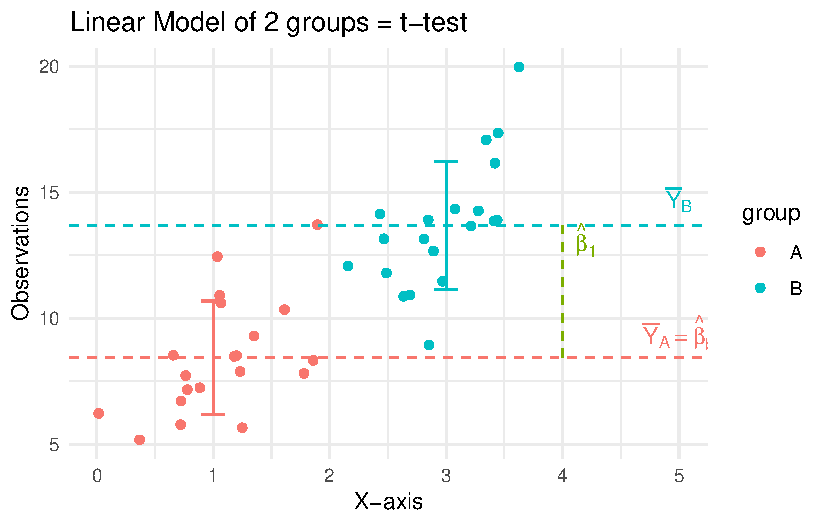
\includegraphics[keepaspectratio]{matrix_files/figure-pdf/unnamed-chunk-58-1.pdf}}
\end{center}

\[
\bar{Y_A} = \hat{\beta_0} 
\] \[
\bar{Y_B}= \hat{\beta_0}+\hat{\beta_1}
\] \[
\bar{Y_A} = 1 \times \hat{\beta_0}+ 0 \times \hat{\beta_1}
\] \[
\bar{Y_B}= 1 \times \hat{\beta_0}+ 1 \times \hat{\beta_1}
\]

And if we had three groups:

\[
\bar{Y_A} = \hat{\beta_0}
\] \[
\bar{Y_B}= \hat{\beta_0}+\hat{\beta_1}
\] \[
\bar{Y_C}= \hat{\beta_0}+\hat{\beta_2}
\] \[
\bar{Y_A} = 1 \times \hat{\beta_0}+ 0 \times \hat{\beta_1}+0 \times\hat{\beta_2} 
\]

\[
\bar{Y_B}= 1 \times \hat{\beta_0}+ 1 \times \hat{\beta_1}+0 \times\hat{\beta_2}
\] \[
\bar{Y_C}= 1 \times \hat{\beta_0}+ 0 \times \hat{\beta_1}+1 \times\hat{\beta_2}
\] how can we create this using r:

\begin{Shaded}
\begin{Highlighting}[]
\NormalTok{x}\OtherTok{\textless{}{-}} \FunctionTok{factor}\NormalTok{(}\FunctionTok{c}\NormalTok{(}\DecValTok{1}\NormalTok{,}\DecValTok{1}\NormalTok{,}\DecValTok{2}\NormalTok{,}\DecValTok{2}\NormalTok{,}\DecValTok{3}\NormalTok{,}\DecValTok{3}\NormalTok{))}
\FunctionTok{model.matrix}\NormalTok{(}\SpecialCharTok{\textasciitilde{}}\NormalTok{ x)}
\end{Highlighting}
\end{Shaded}

\begin{verbatim}
  (Intercept) x2 x3
1           1  0  0
2           1  0  0
3           1  1  0
4           1  1  0
5           1  0  1
6           1  0  1
attr(,"assign")
[1] 0 1 1
attr(,"contrasts")
attr(,"contrasts")$x
[1] "contr.treatment"
\end{verbatim}

with two parameters:

\begin{Shaded}
\begin{Highlighting}[]
\NormalTok{x}\OtherTok{\textless{}{-}} \FunctionTok{factor}\NormalTok{(}\FunctionTok{c}\NormalTok{(}\DecValTok{1}\NormalTok{,}\DecValTok{1}\NormalTok{,}\DecValTok{1}\NormalTok{,}\DecValTok{1}\NormalTok{,}\DecValTok{2}\NormalTok{,}\DecValTok{2}\NormalTok{,}\DecValTok{2}\NormalTok{))}
\NormalTok{y}\OtherTok{\textless{}{-}} \FunctionTok{factor}\NormalTok{(}\FunctionTok{c}\NormalTok{(}\StringTok{"a"}\NormalTok{,}\StringTok{"a"}\NormalTok{,}\StringTok{"b"}\NormalTok{,}\StringTok{"b"}\NormalTok{,}\StringTok{"a"}\NormalTok{,}\StringTok{"a"}\NormalTok{,}\StringTok{"b"}\NormalTok{))}
\FunctionTok{cbind}\NormalTok{(}\FunctionTok{as.character}\NormalTok{(x),}\FunctionTok{as.character}\NormalTok{(y))}
\end{Highlighting}
\end{Shaded}

\begin{verbatim}
     [,1] [,2]
[1,] "1"  "a" 
[2,] "1"  "a" 
[3,] "1"  "b" 
[4,] "1"  "b" 
[5,] "2"  "a" 
[6,] "2"  "a" 
[7,] "2"  "b" 
\end{verbatim}

\begin{Shaded}
\begin{Highlighting}[]
\FunctionTok{model.matrix}\NormalTok{(}\SpecialCharTok{\textasciitilde{}}\NormalTok{ x}\SpecialCharTok{+}\NormalTok{y)}
\end{Highlighting}
\end{Shaded}

\begin{verbatim}
  (Intercept) x2 yb
1           1  0  0
2           1  0  0
3           1  0  1
4           1  0  1
5           1  1  0
6           1  1  0
7           1  1  1
attr(,"assign")
[1] 0 1 2
attr(,"contrasts")
attr(,"contrasts")$x
[1] "contr.treatment"

attr(,"contrasts")$y
[1] "contr.treatment"
\end{verbatim}

and we can compute some calculations if we want using \texttt{I()}

\begin{Shaded}
\begin{Highlighting}[]
\NormalTok{x}\OtherTok{\textless{}{-}}\FunctionTok{c}\NormalTok{(}\DecValTok{1}\NormalTok{,}\DecValTok{2}\NormalTok{,}\DecValTok{3}\NormalTok{,}\DecValTok{4}\NormalTok{,}\DecValTok{5}\NormalTok{)}
\FunctionTok{model.matrix}\NormalTok{(}\SpecialCharTok{\textasciitilde{}}\NormalTok{x }\SpecialCharTok{+}\FunctionTok{I}\NormalTok{(x}\SpecialCharTok{\^{}}\DecValTok{2}\NormalTok{))}
\end{Highlighting}
\end{Shaded}

\begin{verbatim}
  (Intercept) x I(x^2)
1           1 1      1
2           1 2      4
3           1 3      9
4           1 4     16
5           1 5     25
attr(,"assign")
[1] 0 1 2
\end{verbatim}

example: Suppose we have an experiment with the following design: on
three different days, we perform an experiment with two treated and two
control samples. We then measure some outcome \(y_i\) and we want to
test the effect of condition, while controlling for whatever differences
might have occurred due to the different day. Assume that the true
condition effect is the same for each day:

\begin{Shaded}
\begin{Highlighting}[]
\NormalTok{day}\OtherTok{\textless{}{-}} \FunctionTok{c}\NormalTok{(}\StringTok{"A"}\NormalTok{,}\StringTok{"B"}\NormalTok{,}\StringTok{"C"}\NormalTok{)}
\NormalTok{treated}\OtherTok{\textless{}{-}} \FunctionTok{c}\NormalTok{(}\DecValTok{2}\NormalTok{,}\DecValTok{2}\NormalTok{,}\DecValTok{2}\NormalTok{)}
\NormalTok{control}\OtherTok{\textless{}{-}}\FunctionTok{c}\NormalTok{(}\DecValTok{2}\NormalTok{,}\DecValTok{2}\NormalTok{,}\DecValTok{2}\NormalTok{)}
\end{Highlighting}
\end{Shaded}

produce a design matrix that let's us analyse the effect of condition,
controlling for the different days:

\begin{Shaded}
\begin{Highlighting}[]
\NormalTok{condition}\OtherTok{\textless{}{-}} \FunctionTok{cbind}\NormalTok{(}\FunctionTok{factor}\NormalTok{(treated),}\FunctionTok{factor}\NormalTok{(control))}
\FunctionTok{model.matrix}\NormalTok{(}\SpecialCharTok{\textasciitilde{}}\FunctionTok{factor}\NormalTok{(day)}\SpecialCharTok{+}\NormalTok{condition)}
\end{Highlighting}
\end{Shaded}

\begin{verbatim}
  (Intercept) factor(day)B factor(day)C condition1 condition2
1           1            0            0          1          1
2           1            1            0          1          1
3           1            0            1          1          1
attr(,"assign")
[1] 0 1 1 2 2
attr(,"contrasts")
attr(,"contrasts")$`factor(day)`
[1] "contr.treatment"
\end{verbatim}

Example:

we are going to use the dataset of female mice bodyweight to see how
matrices apply to linear models.

We load the dataset and create the matrix. Notice how we can change the
reference level using relevel or factor, this will change which values
for the variable diet get 0 and which ones get a 1. We will usually use
the control group as our reference group.

\begin{Shaded}
\begin{Highlighting}[]
\NormalTok{femaleMiceWeights }\OtherTok{\textless{}{-}} \FunctionTok{read\_csv}\NormalTok{(}\StringTok{"data/femaleMiceWeights.csv"}\NormalTok{)}
\FunctionTok{View}\NormalTok{(femaleMiceWeights)}


\FunctionTok{stripchart}\NormalTok{(femaleMiceWeights}\SpecialCharTok{$}\NormalTok{Bodyweight }\SpecialCharTok{\textasciitilde{}}\NormalTok{ femaleMiceWeights}\SpecialCharTok{$}\NormalTok{Diet,}
  \AttributeTok{vertical=} \ConstantTok{TRUE}\NormalTok{, }\AttributeTok{method =} \StringTok{"jitter"}\NormalTok{,}
  \AttributeTok{main =} \StringTok{"Bodyweight over Diet"}\NormalTok{)}
\end{Highlighting}
\end{Shaded}

\begin{center}
\pandocbounded{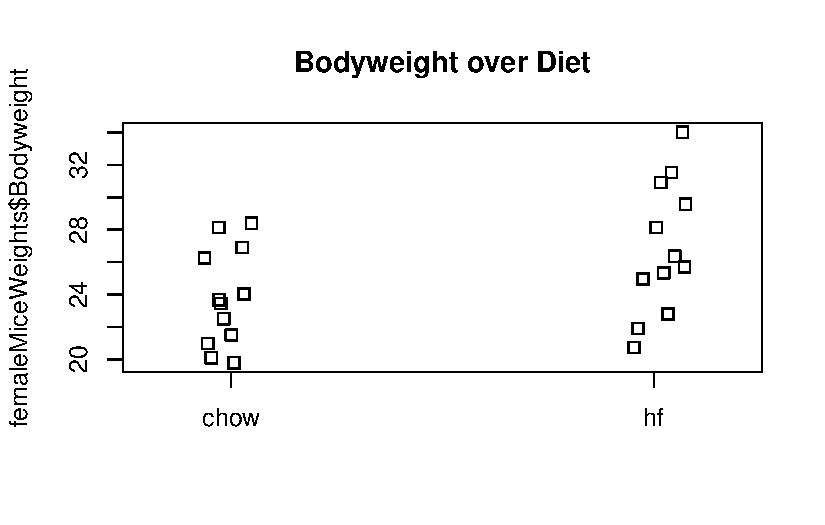
\includegraphics[keepaspectratio]{matrix_files/figure-pdf/unnamed-chunk-64-1.pdf}}
\end{center}

\begin{Shaded}
\begin{Highlighting}[]
\FunctionTok{model.matrix}\NormalTok{(}\SpecialCharTok{\textasciitilde{}}\NormalTok{ Diet, }\AttributeTok{data=}\NormalTok{ femaleMiceWeights)}
\end{Highlighting}
\end{Shaded}

\begin{verbatim}
   (Intercept) Diethf
1            1      0
2            1      0
3            1      0
4            1      0
5            1      0
6            1      0
7            1      0
8            1      0
9            1      0
10           1      0
11           1      0
12           1      0
13           1      1
14           1      1
15           1      1
16           1      1
17           1      1
18           1      1
19           1      1
20           1      1
21           1      1
22           1      1
23           1      1
24           1      1
attr(,"assign")
[1] 0 1
attr(,"contrasts")
attr(,"contrasts")$Diet
[1] "contr.treatment"
\end{verbatim}

if we run a linear model over the data:

\begin{Shaded}
\begin{Highlighting}[]
\NormalTok{fit }\OtherTok{\textless{}{-}} \FunctionTok{lm}\NormalTok{(Bodyweight }\SpecialCharTok{\textasciitilde{}}\NormalTok{ Diet, }\AttributeTok{data=}\NormalTok{ femaleMiceWeights)}
\FunctionTok{summary}\NormalTok{(fit)}
\end{Highlighting}
\end{Shaded}

\begin{verbatim}

Call:
lm(formula = Bodyweight ~ Diet, data = femaleMiceWeights)

Residuals:
    Min      1Q  Median      3Q     Max 
-6.1042 -2.4358 -0.4138  2.8335  7.1858 

Coefficients:
            Estimate Std. Error t value            Pr(>|t|)    
(Intercept)   23.813      1.039  22.912 <0.0000000000000002 ***
Diethf         3.021      1.470   2.055              0.0519 .  
---
Signif. codes:  0 '***' 0.001 '**' 0.01 '*' 0.05 '.' 0.1 ' ' 1

Residual standard error: 3.6 on 22 degrees of freedom
Multiple R-squared:  0.1611,    Adjusted R-squared:  0.1229 
F-statistic: 4.224 on 1 and 22 DF,  p-value: 0.05192
\end{verbatim}

we see we get in the coefficients part we get a value for each column in
the matrix, in our case one for the intercept and one for the non
reference Diet.\\
The estimate for the Diet hf is 3.021 which means that the difference in
weight between the control group (chow diet) and the high fat diet is
3.021 grams.

The second column gives us the standard error.

The third column gives us a t-value that is the estimate divided by the
standard error \texttt{23.813/1.039} for the intercept and
\texttt{3.021/1.470}

The fourth column gives us a p.value that is the probability of seeing
such a large t-value in absolute value.

The fifth column gives you starts or a dot that symbolizes whether that
p-value is below the usual cut-off significant levels \(\alpha\)

if we want to get only the coefficients we can do it by using
\texttt{coef(fit)}

We know that the maths behind the linear model are \[
\hat{\beta}= (X^t X)^{-1} X^t y
\]

and to prove it with our data:

\begin{Shaded}
\begin{Highlighting}[]
\NormalTok{y}\OtherTok{\textless{}{-}}\NormalTok{ femaleMiceWeights}\SpecialCharTok{$}\NormalTok{Bodyweight}
\NormalTok{X}\OtherTok{\textless{}{-}} \FunctionTok{model.matrix}\NormalTok{(}\SpecialCharTok{\textasciitilde{}}\NormalTok{ Diet, }\AttributeTok{data=}\NormalTok{ femaleMiceWeights)}
\FunctionTok{solve}\NormalTok{(}\FunctionTok{t}\NormalTok{(X) }\SpecialCharTok{\%*\%}\NormalTok{ X) }\SpecialCharTok{\%*\%} \FunctionTok{t}\NormalTok{(X) }\SpecialCharTok{\%*\%}\NormalTok{ y}
\end{Highlighting}
\end{Shaded}

\begin{verbatim}
                 [,1]
(Intercept) 23.813333
Diethf       3.020833
\end{verbatim}

visualizing it:

\begin{Shaded}
\begin{Highlighting}[]
\FunctionTok{stripchart}\NormalTok{(femaleMiceWeights}\SpecialCharTok{$}\NormalTok{Bodyweight }\SpecialCharTok{\textasciitilde{}}\NormalTok{ femaleMiceWeights}\SpecialCharTok{$}\NormalTok{Diet,}
  \AttributeTok{vertical=} \ConstantTok{TRUE}\NormalTok{, }\AttributeTok{method =} \StringTok{"jitter"}\NormalTok{,}
  \AttributeTok{main =} \StringTok{"Bodyweight over Diet"}\NormalTok{,}
  \AttributeTok{ylim=}\FunctionTok{c}\NormalTok{(}\DecValTok{0}\NormalTok{,}\DecValTok{40}\NormalTok{),}
  \AttributeTok{xlim=}\FunctionTok{c}\NormalTok{(}\DecValTok{0}\NormalTok{,}\DecValTok{3}\NormalTok{)}
\NormalTok{ )}
\NormalTok{a}\OtherTok{\textless{}{-}} \SpecialCharTok{{-}}\FloatTok{0.25}
\NormalTok{lgth}\OtherTok{\textless{}{-}}\NormalTok{ .}\DecValTok{1}

\NormalTok{cols}\OtherTok{\textless{}{-}} \FunctionTok{brewer.pal}\NormalTok{(}\DecValTok{3}\NormalTok{,}\StringTok{"Dark2"}\NormalTok{)}
\FunctionTok{abline}\NormalTok{(}\AttributeTok{h=}\DecValTok{0}\NormalTok{)}
\FunctionTok{arrows}\NormalTok{(}\DecValTok{1}\SpecialCharTok{+}\NormalTok{a,}\DecValTok{0}\NormalTok{,}\DecValTok{1}\SpecialCharTok{+}\NormalTok{a, }\CommentTok{\#position}
  \FunctionTok{coef}\NormalTok{(fit)[}\DecValTok{1}\NormalTok{], }\CommentTok{\#where the arrow ends (intercept)}
  \AttributeTok{lwd=}\DecValTok{3}\NormalTok{, }\CommentTok{\#}
  \AttributeTok{col=}\NormalTok{cols[}\DecValTok{1}\NormalTok{], }\CommentTok{\#color}
  \AttributeTok{length=}\NormalTok{ lgth }\CommentTok{\#arrow point size.}
\NormalTok{ )}
\FunctionTok{abline}\NormalTok{(}\AttributeTok{h=}\FunctionTok{coef}\NormalTok{(fit)[}\DecValTok{1}\NormalTok{], }\AttributeTok{col=}\NormalTok{cols[}\DecValTok{1}\NormalTok{]) }\CommentTok{\#intercept (mean of chow)}
\FunctionTok{arrows}\NormalTok{(}\DecValTok{2}\SpecialCharTok{+}\NormalTok{a,}\FunctionTok{coef}\NormalTok{(fit)[}\DecValTok{1}\NormalTok{],}\DecValTok{2}\SpecialCharTok{+}\NormalTok{a,}
  \FunctionTok{coef}\NormalTok{(fit)[}\DecValTok{1}\NormalTok{]}\SpecialCharTok{+}\FunctionTok{coef}\NormalTok{(fit)[}\DecValTok{2}\NormalTok{],}
  \AttributeTok{lwd=}\DecValTok{3}\NormalTok{,}
  \AttributeTok{col=}\NormalTok{cols[}\DecValTok{2}\NormalTok{],}
  \AttributeTok{length=}\NormalTok{ lgth)}
\FunctionTok{abline}\NormalTok{(}\AttributeTok{h=}\FunctionTok{coef}\NormalTok{(fit)[}\DecValTok{1}\NormalTok{]}\SpecialCharTok{+}\FunctionTok{coef}\NormalTok{(fit)[}\DecValTok{2}\NormalTok{], }\AttributeTok{col=}\NormalTok{cols[}\DecValTok{2}\NormalTok{])}
\FunctionTok{legend}\NormalTok{(}\StringTok{"bottomright"}\NormalTok{, }\FunctionTok{names}\NormalTok{(}\FunctionTok{coef}\NormalTok{(fit)), }\AttributeTok{fill=}\NormalTok{cols, }\AttributeTok{cex=}\NormalTok{.}\DecValTok{75}\NormalTok{, }\AttributeTok{bg=}\StringTok{"white"}\NormalTok{)}
\end{Highlighting}
\end{Shaded}

\begin{center}
\pandocbounded{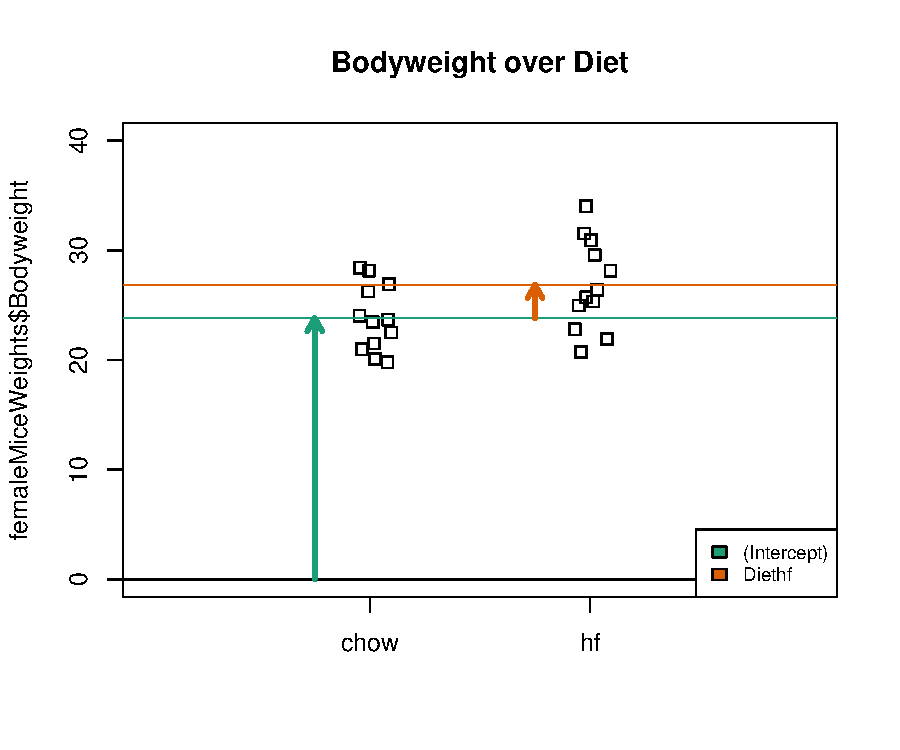
\includegraphics[keepaspectratio]{matrix_files/figure-pdf/unnamed-chunk-67-1.pdf}}
\end{center}

Finally, we can check that we obtain the same results if we run a
t-test:

\begin{Shaded}
\begin{Highlighting}[]
\NormalTok{s}\OtherTok{\textless{}{-}} \FunctionTok{split}\NormalTok{(femaleMiceWeights}\SpecialCharTok{$}\NormalTok{Bodyweight, femaleMiceWeights}\SpecialCharTok{$}\NormalTok{Diet)}
\NormalTok{s}
\end{Highlighting}
\end{Shaded}

\begin{verbatim}
$chow
 [1] 21.51 28.14 24.04 23.45 23.68 19.79 28.40 20.98 22.51 20.10 26.91 26.25

$hf
 [1] 25.71 26.37 22.80 25.34 24.97 28.14 29.58 30.92 34.02 21.90 31.53 20.73
\end{verbatim}

\begin{Shaded}
\begin{Highlighting}[]
\NormalTok{testResult }\OtherTok{\textless{}{-}} \FunctionTok{t.test}\NormalTok{(s[[}\StringTok{"hf"}\NormalTok{]],s[[}\StringTok{"chow"}\NormalTok{]], }\AttributeTok{var.equal=}\ConstantTok{TRUE}\NormalTok{)}
\NormalTok{testResult}
\end{Highlighting}
\end{Shaded}

\begin{verbatim}

    Two Sample t-test

data:  s[["hf"]] and s[["chow"]]
t = 2.0552, df = 22, p-value = 0.05192
alternative hypothesis: true difference in means is not equal to 0
95 percent confidence interval:
 -0.02748516  6.06915183
sample estimates:
mean of x mean of y 
 26.83417  23.81333 
\end{verbatim}

\begin{Shaded}
\begin{Highlighting}[]
\FunctionTok{summary}\NormalTok{(fit)}\SpecialCharTok{$}\NormalTok{coefficients[}\DecValTok{2}\NormalTok{,}\DecValTok{3}\NormalTok{]}
\end{Highlighting}
\end{Shaded}

\begin{verbatim}
[1] 2.055174
\end{verbatim}

\begin{Shaded}
\begin{Highlighting}[]
\NormalTok{testResult}\SpecialCharTok{$}\NormalTok{statistic}
\end{Highlighting}
\end{Shaded}

\begin{verbatim}
       t 
2.055174 
\end{verbatim}

Though the linear model in this case is equivalent to a t-test, we will
soon explore more complicated designs, whre the linear model is a useful
extension (cofounging variables, testing contrast of terms, testing
interactions, testing many terms at once etc.) but for now we can review
the mathematics on why these produce the same t-value and therefore the
same p-value.

We already know that the numerator of the t-value is the difference
between the average of the groups, so we only have to see that the
denominator is also the same. In the linear model, we saw how to
calculate the standard error using the design matrix X and the estimate
of \(\sigma^2\) from the residuals. The estimate of the variance
\(\sigma^2\) was the sum of the squared residuals divided by (N-p) where
N is the total number of samples and p is the number of terms (in our
example an intercept and a group indicator so p=2).

In the t-test, the denominator of the t-value is the standard error of
the difference.

The t-test formula for the standard error of the difference, if we
assume equal variance in the two groups is:

\[
SE =\sqrt{var(diff)} = \sqrt{\sigma_{\Delta}^2}
\] and we know that: \[
\sigma^2 = \frac{1}{N}\sum^N_{i=1}(x_i-\mu)^ 2
\]

now the \emph{variance of the difference between the means of two
samples}:

\[
var(diff) = \left(\frac{1}{n_x}+\frac{1}{n_y}\right)\frac {\sum{(x_i -\mu_x)^2}+ \sum{(y_i- \mu_y)^2}}{(n_x+n_y-2)}
\]

this formula calculates the variance of the difference between two
sample means where - \(n_x\) and \(n_y\) are the sample sizes of the two
groups. - \(x_i\) and \(y_i\) are individual data points within each
group

\begin{itemize}
\item
  \(\mu_x\) and \(\mu_y\) are the means of the two groups.
\item
  \((\frac{1}{n_x}+\frac{1}{n_y})\) adjusts for the sample sizes.
\item
  \(\sum{(x_i -\mu_x)^2}+ \sum{(y_i- \mu_y)}^2\) this sums up the
  squared deviations from the mean for each group.
\item
  \(\frac {\sum{(x_i -\mu_x)^2}+ \sum{(y_i- \mu_y)^2}}{(n_x+n_y-2)}\)
  this calculates the pooled variance, considering both groups together.
\item
  \texttt{2} is the degrees of freedom for the pooled variance
  calculation.
\end{itemize}

The variance of the difference tells you how spread out the difference
between the group means are likely to be.

The standard Error of the estimated coefficient \(\hat{\beta}\) is : \[
se(\hat{\beta})=\sqrt{s^2(X^TX)^{-1}_{ii}}
\] where \((X^TX)^{-1}_{ii}\) is the i-th diagonal element of this
inverse matrix, which corresponds to the variance of the i-th
coefficient estimate.

\subsection{Crossed designs}\label{crossed-designs}

imagine we are running an experiment and we have two different
treatments, group A is the control group and receives no treatment (a),
group B receives treatment 1 (b), group C receives treatment 2 (c) and a
fourth group receives treatment 1 and 2 (d). In this case we consider
the effects of receiving both treatments additive. If we write down a
model it will look like this: \[
\begin{pmatrix}
\color{red}1 & \color{red}0 & \color{red}0 \\
\color{red}1 & \color{red}0 & \color{red}0 \\
\color{blue}1 & \color{blue}1 & \color{blue}0 \\
\color{blue}1 & \color{blue}1 & \color{blue}0 \\
\color{green}1 & \color{green}0 & \color{green}1 \\
\color{green}1 & \color{green}0 & \color{green}1 \\
1 & 1 & 1 \\
1 & 1 & 1
\end{pmatrix}
\begin{pmatrix}
\color{red}{\beta_0 }\\
\color{blue}{\beta_1 }\\
\color{green}{\beta_2}
\end{pmatrix}
\]

we can see that the first two rows are no treatment, the rows 3rd and
4th receive treatment 1 but no treatment 2 , the 5th and the 6th rows
receive treatment 2 but no treatment 1 and the last two rows receive
both treatments.

If the effects of treatment 1 + treatment 2 are not additive, then we
need to plug in a fourth element that will gives us a different mean for
each group and we call that fourth term \emph{interaction}

\[
\begin{pmatrix}
1 & 0 & 0 & 0\\
1 & 1 & 0 & 0\\
1 & 0 & 1 & 0\\
1 & 1 & 0 & 0\\
1 & 0 & 0 & 0\\
1 & 1 & 1 & 0\\
1 & 0 & 1 & 1\\
1 & 1 & 1 & 1
\end{pmatrix}
\begin{pmatrix}
\beta_0 \\
\beta_1 \\
\beta_2\\
\beta_{1:2}
\end{pmatrix}
\]

\section{Interactions and Contrast}\label{interactions-and-contrast}

As a running example to learn about more complex linear models, we will
be using a dataset which compares the different frictional coefficients
on the different legs of a spider. Specifically, we will be determining
whether more friction comes from a pushing or pulling motion of the leg.

To remind ourselves how the simple two-group linear model looks, we will
subset the data to include only the L1 leg pair, and run \texttt{lm}:

\begin{Shaded}
\begin{Highlighting}[]
\NormalTok{spider }\OtherTok{\textless{}{-}} \FunctionTok{read.csv2}\NormalTok{(}\StringTok{"data/spider\_wolff\_gorb\_2013.csv"}\NormalTok{)  }
\NormalTok{spider}\SpecialCharTok{$}\NormalTok{friction }\OtherTok{\textless{}{-}} \FunctionTok{as.numeric}\NormalTok{(spider}\SpecialCharTok{$}\NormalTok{friction)}
\NormalTok{spider.sub }\OtherTok{\textless{}{-}}\NormalTok{ spider[spider}\SpecialCharTok{$}\NormalTok{leg }\SpecialCharTok{==} \StringTok{"L1"}\NormalTok{,]}
\NormalTok{fit }\OtherTok{\textless{}{-}} \FunctionTok{lm}\NormalTok{(friction }\SpecialCharTok{\textasciitilde{}}\NormalTok{ type, }\AttributeTok{data=}\NormalTok{spider.sub)}
\FunctionTok{summary}\NormalTok{(fit)}
\end{Highlighting}
\end{Shaded}

\begin{verbatim}

Call:
lm(formula = friction ~ type, data = spider.sub)

Residuals:
     Min       1Q   Median       3Q      Max 
-0.33147 -0.10735 -0.04941 -0.00147  0.76853 

Coefficients:
            Estimate Std. Error t value             Pr(>|t|)    
(Intercept)  0.92147    0.03827  24.078 < 0.0000000000000002 ***
typepush    -0.51412    0.05412  -9.499    0.000000000000057 ***
---
Signif. codes:  0 '***' 0.001 '**' 0.01 '*' 0.05 '.' 0.1 ' ' 1

Residual standard error: 0.2232 on 66 degrees of freedom
Multiple R-squared:  0.5776,    Adjusted R-squared:  0.5711 
F-statistic: 90.23 on 1 and 66 DF,  p-value: 0.00000000000005698
\end{verbatim}

\begin{Shaded}
\begin{Highlighting}[]
\NormalTok{(coefs }\OtherTok{\textless{}{-}} \FunctionTok{coef}\NormalTok{(fit))}
\end{Highlighting}
\end{Shaded}

\begin{verbatim}
(Intercept)    typepush 
  0.9214706  -0.5141176 
\end{verbatim}

These two estimated coefficients are the mean of the pull observations
(the first estimated coefficient) and the difference between the means
of the two groups (the second coefficient). We can show this with R
code:

\begin{Shaded}
\begin{Highlighting}[]
\NormalTok{s }\OtherTok{\textless{}{-}} \FunctionTok{split}\NormalTok{(spider.sub}\SpecialCharTok{$}\NormalTok{friction, spider.sub}\SpecialCharTok{$}\NormalTok{type)}
\FunctionTok{mean}\NormalTok{(s[[}\StringTok{"pull"}\NormalTok{]])}
\end{Highlighting}
\end{Shaded}

\begin{verbatim}
[1] 0.9214706
\end{verbatim}

\begin{Shaded}
\begin{Highlighting}[]
\FunctionTok{mean}\NormalTok{(s[[}\StringTok{"push"}\NormalTok{]]) }\SpecialCharTok{{-}} \FunctionTok{mean}\NormalTok{(s[[}\StringTok{"pull"}\NormalTok{]])}
\end{Highlighting}
\end{Shaded}

\begin{verbatim}
[1] -0.5141176
\end{verbatim}

We can form the design matrix, which was used inside \texttt{lm}:

\begin{Shaded}
\begin{Highlighting}[]
\NormalTok{X }\OtherTok{\textless{}{-}} \FunctionTok{model.matrix}\NormalTok{(}\SpecialCharTok{\textasciitilde{}}\NormalTok{ type, }\AttributeTok{data=}\NormalTok{spider.sub)}
\FunctionTok{colnames}\NormalTok{(X)}
\end{Highlighting}
\end{Shaded}

\begin{verbatim}
[1] "(Intercept)" "typepush"   
\end{verbatim}

\begin{Shaded}
\begin{Highlighting}[]
\FunctionTok{head}\NormalTok{(X)}
\end{Highlighting}
\end{Shaded}

\begin{verbatim}
  (Intercept) typepush
1           1        0
2           1        0
3           1        0
4           1        0
5           1        0
6           1        0
\end{verbatim}

\begin{Shaded}
\begin{Highlighting}[]
\FunctionTok{tail}\NormalTok{(X)}
\end{Highlighting}
\end{Shaded}

\begin{verbatim}
   (Intercept) typepush
63           1        1
64           1        1
65           1        1
66           1        1
67           1        1
68           1        1
\end{verbatim}

Now we'll make a plot of the \(\mathbf{X}\) matrix by putting a black
block for the 1's and a white block for the 0's. This plot will be more
interesting for the linear models later on in this script. Along the
y-axis is the sample number (the row number of the \texttt{data}) and
along the x-axis is the column of the design matrix \(\mathbf{X}\). If
you have installed the \emph{rafalib} library, you can make this plot
with the \texttt{imagemat} function:

\begin{Shaded}
\begin{Highlighting}[]
\FunctionTok{imagemat}\NormalTok{(X, }\AttributeTok{main=}\StringTok{"Model matrix for linear model with one variable"}\NormalTok{)}
\end{Highlighting}
\end{Shaded}

\begin{figure}[H]

{\centering \pandocbounded{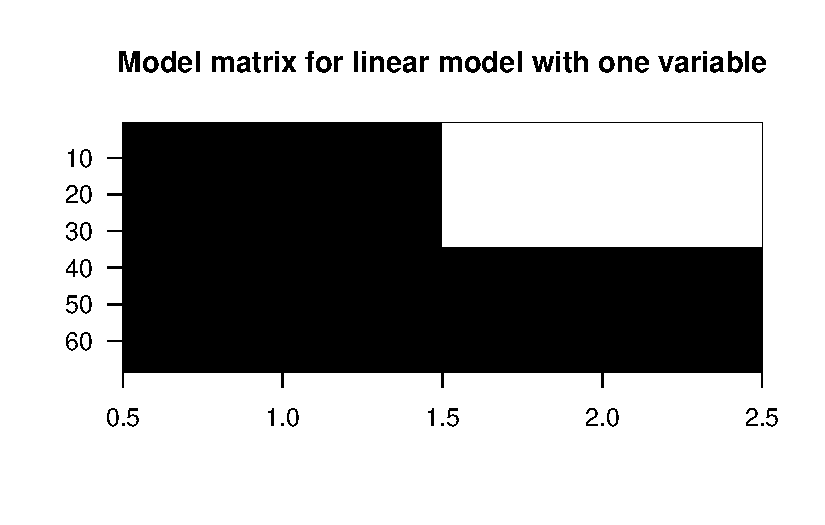
\includegraphics[keepaspectratio]{matrix_files/figure-pdf/model_matrix_image-1.pdf}}

}

\caption{Model matrix for linear model with one variable.}

\end{figure}%

The black represent a 1 and the white represents 0 in the matrix.

We can visualize the data in a strip plot as well

\begin{figure}[H]

{\centering \pandocbounded{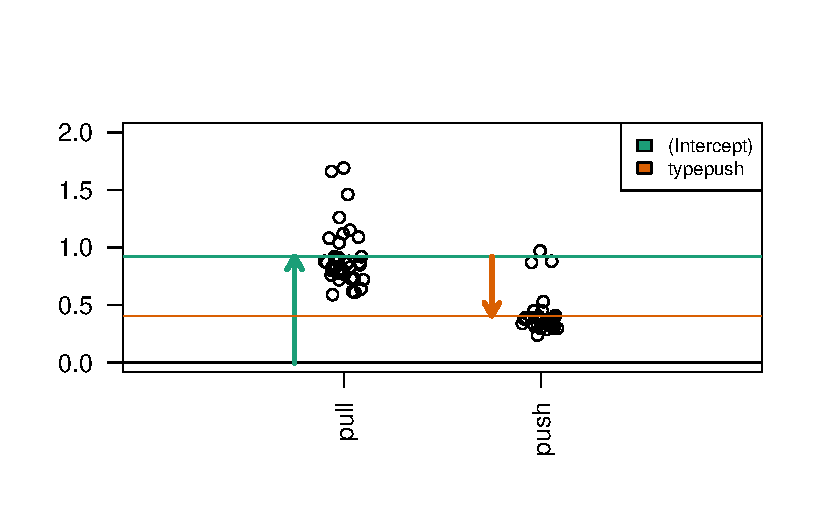
\includegraphics[keepaspectratio]{matrix_files/figure-pdf/spider_main_coef-1.pdf}}

}

\caption{Diagram of the estimated coefficients in the linear model. The
green arrow indicates the Intercept term, which goes from zero to the
mean of the reference group (here the `pull' samples). The orange arrow
indicates the difference between the push group and the pull group,
which is negative in this example. The circles show the individual
samples}

\end{figure}%

\subsection{linear model with two
variables}\label{linear-model-with-two-variables}

Now we are going to use the 4 pairs of legs to show a more complex
linear model.

\begin{Shaded}
\begin{Highlighting}[]
\NormalTok{X }\OtherTok{\textless{}{-}} \FunctionTok{model.matrix}\NormalTok{(}\SpecialCharTok{\textasciitilde{}}\NormalTok{ type }\SpecialCharTok{+}\NormalTok{ leg, }\AttributeTok{data=}\NormalTok{spider)}
\FunctionTok{colnames}\NormalTok{(X)}
\end{Highlighting}
\end{Shaded}

\begin{verbatim}
[1] "(Intercept)" "typepush"    "legL2"       "legL3"       "legL4"      
\end{verbatim}

\begin{Shaded}
\begin{Highlighting}[]
\FunctionTok{head}\NormalTok{(X)}
\end{Highlighting}
\end{Shaded}

\begin{verbatim}
  (Intercept) typepush legL2 legL3 legL4
1           1        0     0     0     0
2           1        0     0     0     0
3           1        0     0     0     0
4           1        0     0     0     0
5           1        0     0     0     0
6           1        0     0     0     0
\end{verbatim}

\begin{Shaded}
\begin{Highlighting}[]
\FunctionTok{imagemat}\NormalTok{(X, }\AttributeTok{main=}\StringTok{"Model matrix for linear model with two factors"}\NormalTok{)}
\end{Highlighting}
\end{Shaded}

\begin{figure}[H]

{\centering \pandocbounded{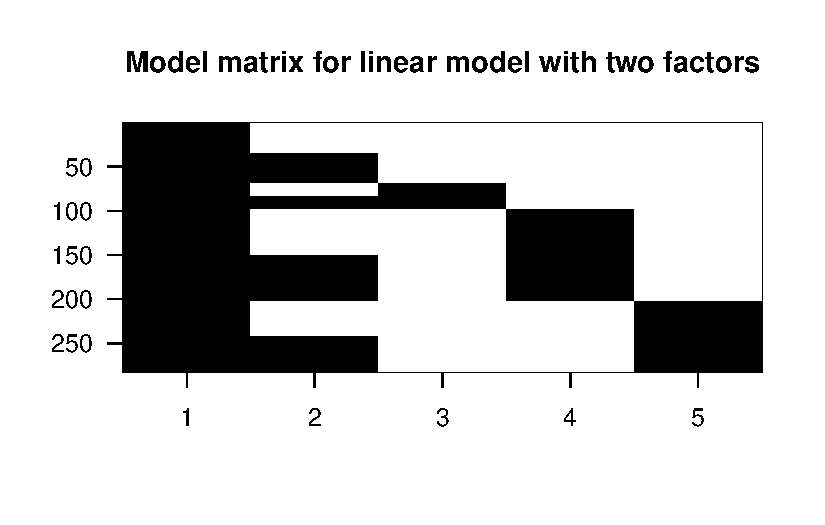
\includegraphics[keepaspectratio]{matrix_files/figure-pdf/model_matrix_image2-1.pdf}}

}

\caption{Image of the model matrix for a formula with type + leg}

\end{figure}%

We have a row for each data point. The first column is the intercept,
and so it has 1's (black) for all samples. The second column expresses
if the data is for a pull or push: it has 1's for the push samples, and
we can see that there are four groups of them (one for each pair of
legs). Finally, the third, fourth and fifth columns expresses what leg
pair we are referencing and have 1's for the L2, L3 and L4 samples. The
L1 samples do not have a column, because \emph{L1} is the reference
level for \texttt{leg}. Similarly, there is no \emph{pull} column,
because \emph{pull} is the reference level for the \texttt{type}
variable.

To estimate coefficients for this model, we use \texttt{lm} with the
formula \texttt{\textasciitilde{}\ type\ +\ leg}. We'll save the linear
model to \texttt{fitTL} standing for a \emph{fit} with \emph{Type} and
\emph{Leg}.

\begin{Shaded}
\begin{Highlighting}[]
\NormalTok{fitTL }\OtherTok{\textless{}{-}} \FunctionTok{lm}\NormalTok{(friction }\SpecialCharTok{\textasciitilde{}}\NormalTok{ type }\SpecialCharTok{+}\NormalTok{ leg, }\AttributeTok{data=}\NormalTok{spider)}
\FunctionTok{summary}\NormalTok{(fitTL)}
\end{Highlighting}
\end{Shaded}

\begin{verbatim}

Call:
lm(formula = friction ~ type + leg, data = spider)

Residuals:
     Min       1Q   Median       3Q      Max 
-0.46392 -0.13441 -0.00525  0.10547  0.69509 

Coefficients:
            Estimate Std. Error t value             Pr(>|t|)    
(Intercept)  1.05392    0.02816  37.426 < 0.0000000000000002 ***
typepush    -0.77901    0.02482 -31.380 < 0.0000000000000002 ***
legL2        0.17192    0.04569   3.763             0.000205 ***
legL3        0.16049    0.03251   4.937   0.0000013710214077 ***
legL4        0.28134    0.03438   8.183   0.0000000000000101 ***
---
Signif. codes:  0 '***' 0.001 '**' 0.01 '*' 0.05 '.' 0.1 ' ' 1

Residual standard error: 0.2084 on 277 degrees of freedom
Multiple R-squared:  0.7916,    Adjusted R-squared:  0.7886 
F-statistic:   263 on 4 and 277 DF,  p-value: < 0.00000000000000022
\end{verbatim}

\begin{Shaded}
\begin{Highlighting}[]
\NormalTok{(coefs }\OtherTok{\textless{}{-}} \FunctionTok{coef}\NormalTok{(fitTL))}
\end{Highlighting}
\end{Shaded}

\begin{verbatim}
(Intercept)    typepush       legL2       legL3       legL4 
  1.0539153  -0.7790071   0.1719216   0.1604921   0.2813382 
\end{verbatim}

R uses the name \texttt{coefficient} to denote the component containing
the least squares \textbf{estimates}. It is important to remember that
the coefficients are parameters that we do not observe, but only
estimate.

We can make the same plot as before, with arrows for each of the
estimated coefficients in the model.

\begin{figure}[H]

{\centering \pandocbounded{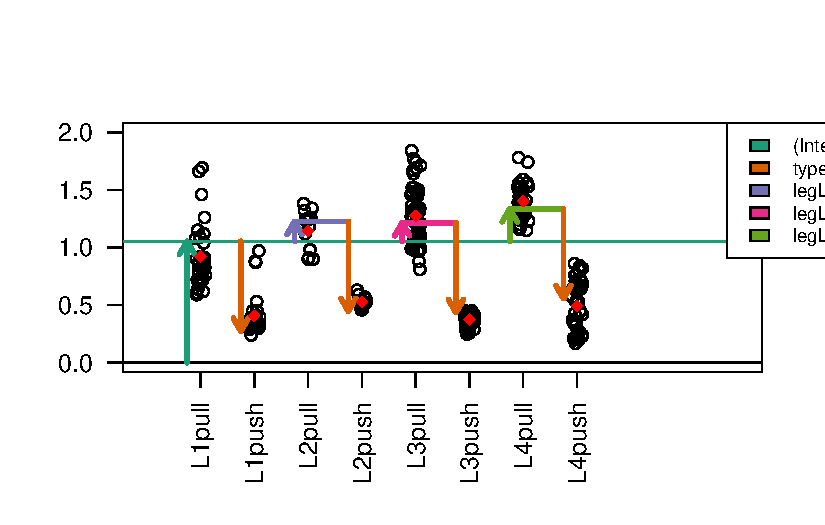
\includegraphics[keepaspectratio]{matrix_files/figure-pdf/spider_interactions-1.pdf}}

}

\caption{Diagram of the estimated coefficients in the linear model. As
before, the teal-green arrow represents the Intercept, which fits the
mean of the reference group (here, the pull samples for leg L1). The
purple, pink, and yellow-green arrows represent differences between the
three other leg groups and L1. The orange arrow represents the
difference between the push and pull samples for all groups.}

\end{figure}%

The intercept is the coefficient for L1 Pull. (dark green) The typepush
is the difference between pull and push. (orange) The LegL2 is the
difference between L1 Pull and L2 Pull The LegL3 is the difference
between L1 Pull and L3 Pull The LegL4 is the difference between L1 Pull
and L4 Pull

The red diamonds represent the mean of each group.

Notice that the intercept is no longer exactly equal to the mean of the
L1 Pull values:

\begin{Shaded}
\begin{Highlighting}[]
\NormalTok{s }\OtherTok{\textless{}{-}} \FunctionTok{split}\NormalTok{(spider}\SpecialCharTok{$}\NormalTok{friction, spider}\SpecialCharTok{$}\NormalTok{group)}
\FunctionTok{cat}\NormalTok{(}\StringTok{\textquotesingle{}mean:\textquotesingle{}}\NormalTok{ , }\FunctionTok{mean}\NormalTok{(s[[}\StringTok{"L1pull"}\NormalTok{]]))}
\end{Highlighting}
\end{Shaded}

\begin{verbatim}
mean: 0.9214706
\end{verbatim}

and same for the other coefficients, the linear model with 8 groups does
not manage to accurately fit the LSE in a way that the coefficients
match the exact mean for each group.

Here we can demonstrate that the push vs.~pull estimated coefficient,
\texttt{coefs{[}2{]}}, is a \emph{weighted average of the difference of
the means for each group}. Furthermore, the weighting is determined by
the sample size of each group. The math works out simply here because
the sample size is equal for the push and pull subgroups within each leg
pair. If the sample sizes were not equal for push and pull within each
leg pair, the weighting is more complicated.

\begin{Shaded}
\begin{Highlighting}[]
\NormalTok{(means }\OtherTok{\textless{}{-}} \FunctionTok{sapply}\NormalTok{(s, mean))}
\end{Highlighting}
\end{Shaded}

\begin{verbatim}
   L1pull    L1push    L2pull    L2push    L3pull    L3push    L4pull    L4push 
0.9214706 0.4073529 1.1453333 0.5273333 1.2738462 0.3759615 1.4007500 0.4907500 
\end{verbatim}

\begin{Shaded}
\begin{Highlighting}[]
\DocumentationTok{\#\#the sample size of push or pull groups for each leg pair}
\NormalTok{ns }\OtherTok{\textless{}{-}} \FunctionTok{sapply}\NormalTok{(s, length)[}\FunctionTok{c}\NormalTok{(}\DecValTok{1}\NormalTok{,}\DecValTok{3}\NormalTok{,}\DecValTok{5}\NormalTok{,}\DecValTok{7}\NormalTok{)]}
\NormalTok{(w }\OtherTok{\textless{}{-}}\NormalTok{ ns}\SpecialCharTok{/}\FunctionTok{sum}\NormalTok{(ns))}
\end{Highlighting}
\end{Shaded}

\begin{verbatim}
   L1pull    L2pull    L3pull    L4pull 
0.2411348 0.1063830 0.3687943 0.2836879 
\end{verbatim}

\begin{Shaded}
\begin{Highlighting}[]
\FunctionTok{sum}\NormalTok{(w }\SpecialCharTok{*}\NormalTok{ (means[}\FunctionTok{c}\NormalTok{(}\DecValTok{2}\NormalTok{,}\DecValTok{4}\NormalTok{,}\DecValTok{6}\NormalTok{,}\DecValTok{8}\NormalTok{)] }\SpecialCharTok{{-}}\NormalTok{ means[}\FunctionTok{c}\NormalTok{(}\DecValTok{1}\NormalTok{,}\DecValTok{3}\NormalTok{,}\DecValTok{5}\NormalTok{,}\DecValTok{7}\NormalTok{)]))}
\end{Highlighting}
\end{Shaded}

\begin{verbatim}
[1] -0.7790071
\end{verbatim}

\begin{Shaded}
\begin{Highlighting}[]
\NormalTok{coefs[}\DecValTok{2}\NormalTok{]}
\end{Highlighting}
\end{Shaded}

\begin{verbatim}
  typepush 
-0.7790071 
\end{verbatim}

\subsection{Contrasting coefficients}\label{contrasting-coefficients}

So all these coefficients are comparing each leg to Leg 1. What do we do
if we want to compare one group to another group that is not the
reference level, for example we want to compare L2 vs L3? We can use the
library \texttt{contrast}

If we want to compare leg pairs L3 and L2, this is equivalent to
contrasting two coefficients from the linear model because, in this
contrast, the comparison to the reference level \emph{L1} cancels out:

\[ (\mbox{L3} - \mbox{L1}) - (\mbox{L2} - \mbox{L1}) = \mbox{L3} - \mbox{L2 }\]

An easy way to make these contrasts of two groups is to use the
\texttt{contrast} function from the \emph{contrast} package. We just
need to specify which groups we want to compare. We have to pick one of
\emph{pull} or \emph{push} types, although the answer will not differ,
as we will see below.

\begin{Shaded}
\begin{Highlighting}[]
\NormalTok{L3vsL2 }\OtherTok{\textless{}{-}}\NormalTok{ contrast}\SpecialCharTok{::}\FunctionTok{contrast}\NormalTok{(fitTL,}\FunctionTok{list}\NormalTok{(}\AttributeTok{leg=}\StringTok{"L3"}\NormalTok{,}\AttributeTok{type=}\StringTok{"pull"}\NormalTok{),}\FunctionTok{list}\NormalTok{(}\AttributeTok{leg=}\StringTok{"L2"}\NormalTok{,}\AttributeTok{type=}\StringTok{"pull"}\NormalTok{))}
\NormalTok{L3vsL2}
\end{Highlighting}
\end{Shaded}

\begin{verbatim}
lm model parameter contrast

    Contrast       S.E.      Lower      Upper     t  df Pr(>|t|)
 -0.01142949 0.04319685 -0.0964653 0.07360632 -0.26 277   0.7915
\end{verbatim}

The first column \texttt{Contrast} gives the L3 vs.~L2 estimate from the
model we fit above.

\begin{Shaded}
\begin{Highlighting}[]
\NormalTok{L3vsL2 }\OtherTok{\textless{}{-}}\NormalTok{ contrast}\SpecialCharTok{::}\FunctionTok{contrast}\NormalTok{(fitTL,}\FunctionTok{list}\NormalTok{(}\AttributeTok{leg=}\StringTok{"L3"}\NormalTok{,}\AttributeTok{type=}\StringTok{"push"}\NormalTok{),}\FunctionTok{list}\NormalTok{(}\AttributeTok{leg=}\StringTok{"L2"}\NormalTok{,}\AttributeTok{type=}\StringTok{"push"}\NormalTok{))}
\NormalTok{L3vsL2}
\end{Highlighting}
\end{Shaded}

\begin{verbatim}
lm model parameter contrast

    Contrast       S.E.      Lower      Upper     t  df Pr(>|t|)
 -0.01142949 0.04319685 -0.0964653 0.07360632 -0.26 277   0.7915
\end{verbatim}

we can check the matrix of the contrast like this:

\begin{Shaded}
\begin{Highlighting}[]
\NormalTok{L3vsL2}\SpecialCharTok{$}\NormalTok{X}
\end{Highlighting}
\end{Shaded}

\begin{verbatim}
  (Intercept) typepush legL2 legL3 legL4
1           0        0    -1     1     0
attr(,"assign")
[1] 0 1 2 2 2
attr(,"contrasts")
attr(,"contrasts")$type
[1] "contr.treatment"

attr(,"contrasts")$leg
[1] "contr.treatment"
\end{verbatim}

and we see that it gives us 0,0,-1,1,0 which means that to find the
contrast we are interested in we need to go take the third coefficient
from the linear model times -1 and sum the 4th coefficient. Let's check
if that applies:

\begin{Shaded}
\begin{Highlighting}[]
\NormalTok{coefs}\OtherTok{\textless{}{-}} \FunctionTok{coef}\NormalTok{(fitTL)}
\SpecialCharTok{{-}}\NormalTok{coefs[}\DecValTok{3}\NormalTok{]}\SpecialCharTok{+}\NormalTok{coefs[}\DecValTok{4}\NormalTok{]}
\end{Highlighting}
\end{Shaded}

\begin{verbatim}
      legL2 
-0.01142949 
\end{verbatim}

\subsection{Linear model with
interactions}\label{linear-model-with-interactions}

In the previous linear model, we assumed that the push vs.~pull effect
was the same for all of the leg pairs (the same orange arrow). You can
easily see that this does not capture the trends in the data that well.
That is, the tips of the arrows did not line up perfectly with the group
averages. For the L1 leg pair, the push vs.~pull estimated coefficient
was too large, and for the L3 leg pair, the push vs.~pull coefficient
was somewhat too small.

\emph{Interaction terms} will help us overcome this problem by
introducing additional coefficients to compensate for differences in the
push vs.~pull effect across the 4 groups. As we already have a push
vs.~pull term in the model, we only need to add three more terms to have
the freedom to find leg-pair-specific push vs.~pull differences. As we
will see, interaction terms are added to the design matrix by
multiplying the columns of the design matrix representing existing
terms.

We can rebuild our linear model with an interaction between
\texttt{type} and \texttt{leg}, by including an extra term in the
formula \texttt{type:leg}. The \texttt{:} symbol adds an interaction
between the two variables surrounding it. An equivalent way to specify
this model is \texttt{\textasciitilde{}\ type*leg}, which will expand to
the formula \texttt{\textasciitilde{}\ type\ +\ leg\ +\ type:leg}, with
main effects for \texttt{type}, \texttt{leg} and an interaction term
\texttt{type:leg}.

\begin{Shaded}
\begin{Highlighting}[]
\NormalTok{X }\OtherTok{\textless{}{-}} \FunctionTok{model.matrix}\NormalTok{(}\SpecialCharTok{\textasciitilde{}}\NormalTok{ type }\SpecialCharTok{+}\NormalTok{ leg }\SpecialCharTok{+}\NormalTok{ type}\SpecialCharTok{:}\NormalTok{leg, }\AttributeTok{data=}\NormalTok{spider)}
\FunctionTok{colnames}\NormalTok{(X)}
\end{Highlighting}
\end{Shaded}

\begin{verbatim}
[1] "(Intercept)"    "typepush"       "legL2"          "legL3"         
[5] "legL4"          "typepush:legL2" "typepush:legL3" "typepush:legL4"
\end{verbatim}

\begin{Shaded}
\begin{Highlighting}[]
\FunctionTok{head}\NormalTok{(X)}
\end{Highlighting}
\end{Shaded}

\begin{verbatim}
  (Intercept) typepush legL2 legL3 legL4 typepush:legL2 typepush:legL3
1           1        0     0     0     0              0              0
2           1        0     0     0     0              0              0
3           1        0     0     0     0              0              0
4           1        0     0     0     0              0              0
5           1        0     0     0     0              0              0
6           1        0     0     0     0              0              0
  typepush:legL4
1              0
2              0
3              0
4              0
5              0
6              0
\end{verbatim}

\begin{Shaded}
\begin{Highlighting}[]
\FunctionTok{imagemat}\NormalTok{(X, }\AttributeTok{main=}\StringTok{"Model matrix for linear model with interactions"}\NormalTok{)}
\end{Highlighting}
\end{Shaded}

\begin{figure}[H]

{\centering \pandocbounded{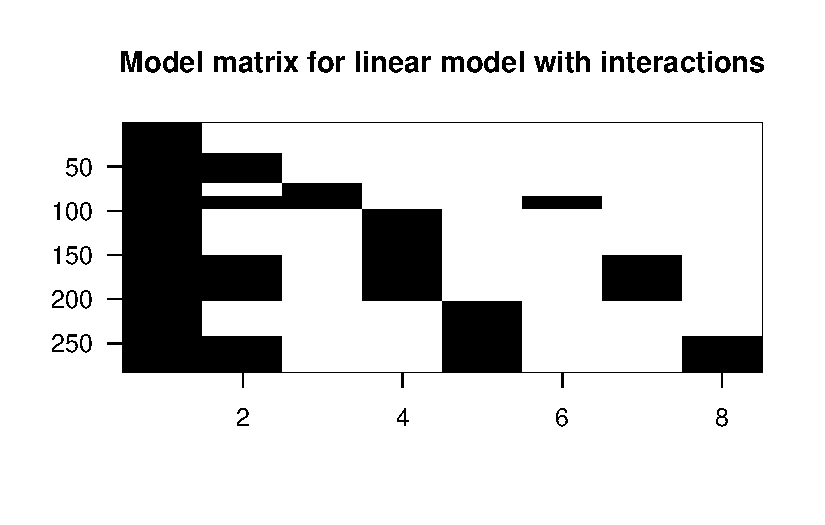
\includegraphics[keepaspectratio]{matrix_files/figure-pdf/model_matrix_with_interaction_image-1.pdf}}

}

\caption{Image of model matrix with interactions.}

\end{figure}%

Columns 6-8 (\texttt{typepush:legL2}, \texttt{typepush:legL3}, and
\texttt{typepush:legL4}) are the product of the 2nd column
(\texttt{typepush}) and columns 3-5 (the three \texttt{leg} columns).
Looking at the last column, for example, the \texttt{typepush:legL4}
column is adding an extra coefficient \(\beta_{\textrm{push,L4}}\) to
those samples which are both push samples and leg pair L4 samples. This
accounts for a possible difference when the mean of samples in the
L4-push group are not at the location which would be predicted by adding
the estimated intercept, the estimated push coefficient
\texttt{typepush}, and the estimated L4 coefficient \texttt{legL4}.

We can run the linear model using the same code as before:

\begin{Shaded}
\begin{Highlighting}[]
\NormalTok{fitX }\OtherTok{\textless{}{-}} \FunctionTok{lm}\NormalTok{(friction }\SpecialCharTok{\textasciitilde{}}\NormalTok{ type }\SpecialCharTok{+}\NormalTok{ leg }\SpecialCharTok{+}\NormalTok{ type}\SpecialCharTok{:}\NormalTok{leg, }\AttributeTok{data=}\NormalTok{spider)}
\FunctionTok{summary}\NormalTok{(fitX)}
\end{Highlighting}
\end{Shaded}

\begin{verbatim}

Call:
lm(formula = friction ~ type + leg + type:leg, data = spider)

Residuals:
     Min       1Q   Median       3Q      Max 
-0.46385 -0.10735 -0.01111  0.07848  0.76853 

Coefficients:
               Estimate Std. Error t value             Pr(>|t|)    
(Intercept)     0.92147    0.03266  28.215 < 0.0000000000000002 ***
typepush       -0.51412    0.04619 -11.131 < 0.0000000000000002 ***
legL2           0.22386    0.05903   3.792             0.000184 ***
legL3           0.35238    0.04200   8.390  0.00000000000000262 ***
legL4           0.47928    0.04442  10.789 < 0.0000000000000002 ***
typepush:legL2 -0.10388    0.08348  -1.244             0.214409    
typepush:legL3 -0.38377    0.05940  -6.461  0.00000000047335813 ***
typepush:legL4 -0.39588    0.06282  -6.302  0.00000000117063701 ***
---
Signif. codes:  0 '***' 0.001 '**' 0.01 '*' 0.05 '.' 0.1 ' ' 1

Residual standard error: 0.1904 on 274 degrees of freedom
Multiple R-squared:  0.8279,    Adjusted R-squared:  0.8235 
F-statistic: 188.3 on 7 and 274 DF,  p-value: < 0.00000000000000022
\end{verbatim}

\begin{Shaded}
\begin{Highlighting}[]
\NormalTok{coefs }\OtherTok{\textless{}{-}} \FunctionTok{coef}\NormalTok{(fitX)}
\end{Highlighting}
\end{Shaded}

Here is where the plot with arrows really helps us interpret the
coefficients. The estimated interaction coefficients (the yellow, brown
and silver arrows) allow leg-pair-specific differences in the push
vs.~pull difference. The orange arrow now represents the estimated push
vs.~pull difference only for the reference leg pair, which is L1. If an
estimated interaction coefficient is large, this means that the push
vs.~pull difference for that leg pair is very different than the push
vs.~pull difference in the reference leg pair.

Now, as we have eight terms in the model and eight parameters, you can
check that the tips of the arrowheads are exactly equal to the group
means (code not shown).

\begin{figure}[H]

{\centering \pandocbounded{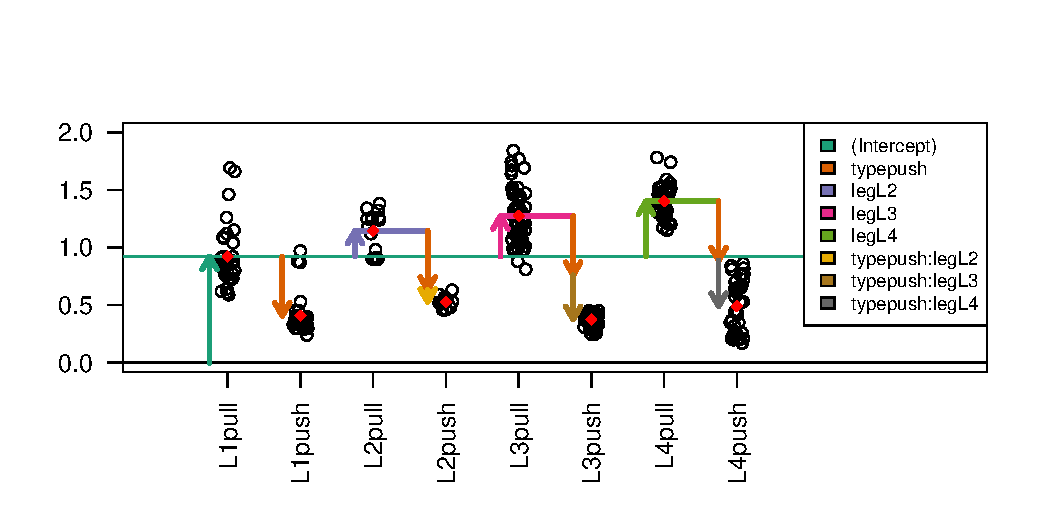
\includegraphics[keepaspectratio]{matrix_files/figure-pdf/spider_interactions2-1.pdf}}

}

\caption{Diagram of the estimated coefficients in the linear model. In
the design with interaction terms, the orange arrow now indicates the
push vs.~pull difference only for the reference group (L1), while three
new arrows (yellow, brown and grey) indicate the additional push
vs.~pull differences in the non-reference groups (L2, L3 and L4) with
respect to the reference group.}

\end{figure}%

Now we want to compare push vs pull in L2:

\begin{Shaded}
\begin{Highlighting}[]
\NormalTok{L2push.vs.pull }\OtherTok{\textless{}{-}}\NormalTok{ contrast}\SpecialCharTok{::}\FunctionTok{contrast}\NormalTok{(fitX,}
  \FunctionTok{list}\NormalTok{(}\AttributeTok{leg=}\StringTok{"L2"}\NormalTok{, }\AttributeTok{type =} \StringTok{"push"}\NormalTok{),}
  \FunctionTok{list}\NormalTok{(}\AttributeTok{leg=}\StringTok{"L2"}\NormalTok{, }\AttributeTok{type =} \StringTok{"pull"}\NormalTok{)}
\NormalTok{)}
\NormalTok{L2push.vs.pull}
\end{Highlighting}
\end{Shaded}

\begin{verbatim}
lm model parameter contrast

 Contrast      S.E.      Lower      Upper     t  df Pr(>|t|)
   -0.618 0.0695372 -0.7548951 -0.4811049 -8.89 274        0
\end{verbatim}

we can look at the contrast vector that will be :

\begin{Shaded}
\begin{Highlighting}[]
\NormalTok{(C}\OtherTok{\textless{}{-}}\NormalTok{ L2push.vs.pull}\SpecialCharTok{$}\NormalTok{X)}
\end{Highlighting}
\end{Shaded}

\begin{verbatim}
  (Intercept) typepush legL2 legL3 legL4 typepush:legL2 typepush:legL3
1           0        1     0     0     0              1              0
  typepush:legL4
1              0
attr(,"assign")
[1] 0 1 2 2 2 3 3 3
attr(,"contrasts")
attr(,"contrasts")$type
[1] "contr.treatment"

attr(,"contrasts")$leg
[1] "contr.treatment"
\end{verbatim}

wich is: 0,1,0,0,0,1,0 and means we need to add the 2nd coefficient to
the 6th coefficient

\begin{Shaded}
\begin{Highlighting}[]
\NormalTok{coefs[}\DecValTok{2}\NormalTok{]}\SpecialCharTok{+}\NormalTok{coefs[}\DecValTok{6}\NormalTok{]}
\end{Highlighting}
\end{Shaded}

\begin{verbatim}
typepush 
  -0.618 
\end{verbatim}

Now we are interested in comparing if the difference between push and
pull from one leg with the difference between push and pull from another
leg, let's say L3 and L4. This is a differences of differences and we
cannot use the same contrast package. We will use the library
\texttt{multcomp}. Remember we had 8 coefficients from the linear model:

\begin{Shaded}
\begin{Highlighting}[]
\NormalTok{coefs}
\end{Highlighting}
\end{Shaded}

\begin{verbatim}
   (Intercept)       typepush          legL2          legL3          legL4 
     0.9214706     -0.5141176      0.2238627      0.3523756      0.4792794 
typepush:legL2 typepush:legL3 typepush:legL4 
    -0.1038824     -0.3837670     -0.3958824 
\end{verbatim}

If we look in the plot we are interested in the difference between the
brown line and the yellow line and those are represented by the
coefficients 6 and 7. So we have to construct a matrix with 1 on the
coefficients we are interested in and 0 in the rest:

\begin{Shaded}
\begin{Highlighting}[]
\NormalTok{C}\OtherTok{\textless{}{-}} \FunctionTok{matrix}\NormalTok{(}\FunctionTok{c}\NormalTok{(}\DecValTok{0}\NormalTok{,}\DecValTok{0}\NormalTok{,}\DecValTok{0}\NormalTok{,}\DecValTok{0}\NormalTok{,}\DecValTok{0}\NormalTok{,}\SpecialCharTok{{-}}\DecValTok{1}\NormalTok{,}\DecValTok{1}\NormalTok{,}\DecValTok{0}\NormalTok{),}\DecValTok{1}\NormalTok{)}
\NormalTok{L3vsL2interaction }\OtherTok{\textless{}{-}}\NormalTok{ multcomp}\SpecialCharTok{::}\FunctionTok{glht}\NormalTok{(fitX, }\AttributeTok{linfct=}\NormalTok{C)}
\FunctionTok{summary}\NormalTok{(L3vsL2interaction)}
\end{Highlighting}
\end{Shaded}

\begin{verbatim}

     Simultaneous Tests for General Linear Hypotheses

Fit: lm(formula = friction ~ type + leg + type:leg, data = spider)

Linear Hypotheses:
       Estimate Std. Error t value Pr(>|t|)    
1 == 0 -0.27988    0.07893  -3.546  0.00046 ***
---
Signif. codes:  0 '***' 0.001 '**' 0.01 '*' 0.05 '.' 0.1 ' ' 1
(Adjusted p values reported -- single-step method)
\end{verbatim}

and we see that it is the same as subtracting the coefficients, but the
function above gives us also a t-statistic and a p-value.

\begin{Shaded}
\begin{Highlighting}[]
\NormalTok{coefs[}\DecValTok{7}\NormalTok{]}\SpecialCharTok{{-}}\NormalTok{coefs[}\DecValTok{6}\NormalTok{]}
\end{Highlighting}
\end{Shaded}

\begin{verbatim}
typepush:legL3 
    -0.2798846 
\end{verbatim}

Finally we can ask if the pull vs push difference is different for each
pair of legs, and this can be answered using anova.

\begin{Shaded}
\begin{Highlighting}[]
\FunctionTok{anova}\NormalTok{(fitX)}
\end{Highlighting}
\end{Shaded}

\begin{verbatim}
Analysis of Variance Table

Response: friction
           Df Sum Sq Mean Sq  F value                Pr(>F)    
type        1 42.783  42.783 1179.713 < 0.00000000000000022 ***
leg         3  2.921   0.974   26.847  0.000000000000002972 ***
type:leg    3  2.098   0.699   19.282  0.000000000022555601 ***
Residuals 274  9.937   0.036                                   
---
Signif. codes:  0 '***' 0.001 '**' 0.01 '*' 0.05 '.' 0.1 ' ' 1
\end{verbatim}

the \texttt{Sum\ Sq} column in the anova results is the variance of the
aggregated coefficients and it is telling us what variables are
responsible for the variance, so for example in our results the
\texttt{Sum\ Sq} for the \texttt{type} (push vs pull) is \texttt{42.783}
it's the highest of them all, which means that this is most responsible
for the variance in the coefficients. Then we have a \texttt{Sum\ Sq}
for the leg (in our graph are the purple, pink and green arrows) with a
value of of \texttt{2.921} so they also explain part of the variance.
Finally we also have a \texttt{2.098} value in \texttt{Sum\ Sq} for the
interaction type:leg (push vs pull by Leg pair) (in our graph the
yellow, brown and grey arrows) which means that there is also a
difference attributed to that. The f-value is like the t-value in a
t-test. The p-value works the same as in a t-test, in our case it is
smaller than 0.05 so it means that the difference we are seeing in those
values are more than what we would expect by chance.

\section{Collinearity}\label{collinearity}

If an experiment is designed incorrectly we may not be able to estimate
the parameters of interest. Similarly, when analyzing data we may
incorrectly decide to use a model that can't be fit. If we are using
linear models then we can detect these problems mathematically by
looking for collinearity in the design matrix.

Some system of equations can have more than one solution:

\begin{align*}
a+c &=1\\
b-c &=1\\
a+b &=2
\end{align*}

there are an infinite number of triplets that satisfy \(a=1-c, b=1+c\).

The system of equations above can be written like this:

\[
\,
\begin{pmatrix}
1&0&1\\
0&1&-1\\
1&1&0\\
\end{pmatrix}
\begin{pmatrix}
a\\
b\\
c
\end{pmatrix}
=
\begin{pmatrix}
1\\
1\\
2
\end{pmatrix}
\]

and we can notice that the third column is a linear combination of the
first two: \[
\,
\begin{pmatrix}
1\\
0\\
1
\end{pmatrix}
+
-1 \begin{pmatrix}
0\\
1\\
1
\end{pmatrix}
=
\begin{pmatrix}
1\\
-1\\
0
\end{pmatrix}
\]

The third column does not add a constraint and what we really have are
three equations and two unknowns: \(a+c\) and \(b-c\). Once we have
values for those two quantities, there are an infinity number of
triplets that can be used.

\subsection{Collinearity and Least
Squares}\label{collinearity-and-least-squares}

Consider a design matrix \(\mathbf{X}\) with two collinear columns. Here
we create an extreme example in which one column is the opposite of
another:

\[
\mathbf{X} = \begin{pmatrix}
\mathbf{1}&\mathbf{X}_1&\mathbf{X}_2&\mathbf{X}_3\\
\end{pmatrix}
\mbox{ with, say, }
\mathbf{X}_3 = - \mathbf{X}_2
\]

This means that we can rewrite the residuals like this:

\[
\mathbf{Y}- \left\{ \mathbf{1}\beta_0 + \mathbf{X}_1\beta_1 + \mathbf{X}_2\beta_2 + \mathbf{X}_3\beta_3\right\}\\ 
= \mathbf{Y}- \left\{ \mathbf{1}\beta_0 + \mathbf{X}_1\beta_1 + \mathbf{X}_2\beta_2 - \mathbf{X}_2\beta_3\right\}\\
= \mathbf{Y}- \left\{\mathbf{1}\beta_0 + \mathbf{X}_1 \beta_1 + \mathbf{X}_2(\beta_2  - \beta_3)\right\}
\] so if we have a solution, adding one to both beta2 and beta3 will
also be a solution, so there is not a single value that minimizes the
error.

and if \(\hat{\beta}_1\), \(\hat{\beta}_2\), \(\hat{\beta}_3\) is a
least squares solution, then, for example, \(\hat{\beta}_1\),
\(\hat{\beta}_2+1\), \(\hat{\beta}_3+1\) is also a solution.

\paragraph{Confounding as an example}\label{confounding-as-an-example}

Now we will demonstrate how collinearity helps us determine problems
with our design using one of the most common errors made in current
experimental design: confounding. To illustrate, let's use an imagined
experiment in which we are interested in the effect of four treatments
A, B, C and D. We assign two mice to each treatment. After starting the
experiment by giving A and B to female mice, we realize there might be a
sex effect. We decide to give C and D to males with hopes of estimating
this effect. But can we estimate the sex effect? The described design
implies the following design matrix:

\[
\,
\begin{pmatrix}
Sex & A & B & C & D\\
0 & 1 & 0 & 0 & 0 \\
0 & 1 & 0 & 0 & 0 \\
0 & 0 & 1 & 0 & 0 \\
0 & 0 & 1 & 0 & 0 \\
1 & 0 & 0 & 1 & 0 \\
1 & 0 & 0 & 1 & 0 \\
1 & 0 & 0 & 0 & 1 \\
1 & 0 & 0 & 0 & 1\\
\end{pmatrix}
\]

Here we can see that sex and treatment are confounded. Specifically, the
sex column can be written as a linear combination of the C and D
matrices.

\[
\,
\begin{pmatrix}
Sex \\
0\\
0 \\
0 \\
0 \\
1\\
1\\
1 \\
1 \\
\end{pmatrix}
=
\begin{pmatrix}
C \\
0\\
0\\
0\\
0\\
1\\
1\\
0\\
0\\
\end{pmatrix}
+
\begin{pmatrix}
D \\
0\\
0\\
0\\
0\\
0\\
0\\
1\\
1\\
\end{pmatrix}
\]

This implies that a unique least squares estimate is not achievable.

It can be difficult to perceive that just looking at the matrix. In r we
have a function that will help us with this:

\subsubsection{Rank}\label{rank}

The \emph{rank} of a matrix columns is the number of columns that are
independent of all the others. If the rank is smaller than the number of
columns, then the LSE are not unique. In R, we can obtain the rank of
matrix with the function \texttt{qr}, which we will describe in more
detail in a following section.

\begin{Shaded}
\begin{Highlighting}[]
\NormalTok{Sex }\OtherTok{\textless{}{-}} \FunctionTok{c}\NormalTok{(}\DecValTok{0}\NormalTok{,}\DecValTok{0}\NormalTok{,}\DecValTok{0}\NormalTok{,}\DecValTok{0}\NormalTok{,}\DecValTok{1}\NormalTok{,}\DecValTok{1}\NormalTok{,}\DecValTok{1}\NormalTok{,}\DecValTok{1}\NormalTok{)}
\NormalTok{A }\OtherTok{\textless{}{-}}   \FunctionTok{c}\NormalTok{(}\DecValTok{1}\NormalTok{,}\DecValTok{1}\NormalTok{,}\DecValTok{0}\NormalTok{,}\DecValTok{0}\NormalTok{,}\DecValTok{0}\NormalTok{,}\DecValTok{0}\NormalTok{,}\DecValTok{0}\NormalTok{,}\DecValTok{0}\NormalTok{)}
\NormalTok{B }\OtherTok{\textless{}{-}}   \FunctionTok{c}\NormalTok{(}\DecValTok{0}\NormalTok{,}\DecValTok{0}\NormalTok{,}\DecValTok{1}\NormalTok{,}\DecValTok{1}\NormalTok{,}\DecValTok{0}\NormalTok{,}\DecValTok{0}\NormalTok{,}\DecValTok{0}\NormalTok{,}\DecValTok{0}\NormalTok{)}
\NormalTok{C }\OtherTok{\textless{}{-}}   \FunctionTok{c}\NormalTok{(}\DecValTok{0}\NormalTok{,}\DecValTok{0}\NormalTok{,}\DecValTok{0}\NormalTok{,}\DecValTok{0}\NormalTok{,}\DecValTok{1}\NormalTok{,}\DecValTok{1}\NormalTok{,}\DecValTok{0}\NormalTok{,}\DecValTok{0}\NormalTok{)}
\NormalTok{D }\OtherTok{\textless{}{-}}   \FunctionTok{c}\NormalTok{(}\DecValTok{0}\NormalTok{,}\DecValTok{0}\NormalTok{,}\DecValTok{0}\NormalTok{,}\DecValTok{0}\NormalTok{,}\DecValTok{0}\NormalTok{,}\DecValTok{0}\NormalTok{,}\DecValTok{1}\NormalTok{,}\DecValTok{1}\NormalTok{)}
\NormalTok{X }\OtherTok{\textless{}{-}} \FunctionTok{model.matrix}\NormalTok{(}\SpecialCharTok{\textasciitilde{}}\NormalTok{Sex}\SpecialCharTok{+}\NormalTok{A}\SpecialCharTok{+}\NormalTok{B}\SpecialCharTok{+}\NormalTok{C}\SpecialCharTok{+}\NormalTok{D}\DecValTok{{-}1}\NormalTok{)}
\FunctionTok{cat}\NormalTok{(}\StringTok{"ncol="}\NormalTok{,}\FunctionTok{ncol}\NormalTok{(X),}\StringTok{"rank="}\NormalTok{, }\FunctionTok{qr}\NormalTok{(X)}\SpecialCharTok{$}\NormalTok{rank,}\StringTok{"}\SpecialCharTok{\textbackslash{}n}\StringTok{"}\NormalTok{)}
\end{Highlighting}
\end{Shaded}

\begin{verbatim}
ncol= 5 rank= 4 
\end{verbatim}

This particular experiment could have been designed better. Using the
same number of male and female mice, we can easily design an experiment
that allows us to compute the sex effect as well as all the treatment
effects. Specifically, when we balance sex and treatments, the
confounding is removed as demonstrated by the fact that the rank is now
the same as the number of columns:

\begin{Shaded}
\begin{Highlighting}[]
\NormalTok{Sex }\OtherTok{\textless{}{-}} \FunctionTok{c}\NormalTok{(}\DecValTok{0}\NormalTok{,}\DecValTok{1}\NormalTok{,}\DecValTok{0}\NormalTok{,}\DecValTok{1}\NormalTok{,}\DecValTok{0}\NormalTok{,}\DecValTok{1}\NormalTok{,}\DecValTok{0}\NormalTok{,}\DecValTok{1}\NormalTok{)}
\NormalTok{A }\OtherTok{\textless{}{-}}   \FunctionTok{c}\NormalTok{(}\DecValTok{1}\NormalTok{,}\DecValTok{1}\NormalTok{,}\DecValTok{0}\NormalTok{,}\DecValTok{0}\NormalTok{,}\DecValTok{0}\NormalTok{,}\DecValTok{0}\NormalTok{,}\DecValTok{0}\NormalTok{,}\DecValTok{0}\NormalTok{)}
\NormalTok{B }\OtherTok{\textless{}{-}}   \FunctionTok{c}\NormalTok{(}\DecValTok{0}\NormalTok{,}\DecValTok{0}\NormalTok{,}\DecValTok{1}\NormalTok{,}\DecValTok{1}\NormalTok{,}\DecValTok{0}\NormalTok{,}\DecValTok{0}\NormalTok{,}\DecValTok{0}\NormalTok{,}\DecValTok{0}\NormalTok{)}
\NormalTok{C }\OtherTok{\textless{}{-}}   \FunctionTok{c}\NormalTok{(}\DecValTok{0}\NormalTok{,}\DecValTok{0}\NormalTok{,}\DecValTok{0}\NormalTok{,}\DecValTok{0}\NormalTok{,}\DecValTok{1}\NormalTok{,}\DecValTok{1}\NormalTok{,}\DecValTok{0}\NormalTok{,}\DecValTok{0}\NormalTok{)}
\NormalTok{D }\OtherTok{\textless{}{-}}   \FunctionTok{c}\NormalTok{(}\DecValTok{0}\NormalTok{,}\DecValTok{0}\NormalTok{,}\DecValTok{0}\NormalTok{,}\DecValTok{0}\NormalTok{,}\DecValTok{0}\NormalTok{,}\DecValTok{0}\NormalTok{,}\DecValTok{1}\NormalTok{,}\DecValTok{1}\NormalTok{)}
\NormalTok{X }\OtherTok{\textless{}{-}} \FunctionTok{model.matrix}\NormalTok{(}\SpecialCharTok{\textasciitilde{}}\NormalTok{Sex}\SpecialCharTok{+}\NormalTok{A}\SpecialCharTok{+}\NormalTok{B}\SpecialCharTok{+}\NormalTok{C}\SpecialCharTok{+}\NormalTok{D}\DecValTok{{-}1}\NormalTok{)}
\FunctionTok{cat}\NormalTok{(}\StringTok{"ncol="}\NormalTok{,}\FunctionTok{ncol}\NormalTok{(X),}\StringTok{"rank="}\NormalTok{, }\FunctionTok{qr}\NormalTok{(X)}\SpecialCharTok{$}\NormalTok{rank,}\StringTok{"}\SpecialCharTok{\textbackslash{}n}\StringTok{"}\NormalTok{)}
\end{Highlighting}
\end{Shaded}

\begin{verbatim}
ncol= 5 rank= 5 
\end{verbatim}

Here we will not be able to estimate the effect of sex.




\end{document}
